%! TEX program = lualatex
\documentclass[11pt]{scrartcl}
% Packages
\usepackage[margin=1.25in]{geometry}
\usepackage{index}
\usepackage{amsbsy} % Bold math symbols
\makeindex
%\usepackage[utf8]{inputenc}
\usepackage[T1]{fontenc}
\usepackage{tcolorbox}
\tcbuselibrary{theorems}
\tcbuselibrary{skins}
\tcbuselibrary{breakable}
\usepackage{varwidth}
\usepackage{textcomp}
\usepackage{amsmath, amssymb}
\usepackage{esint}
\usepackage{titlesec}
\usepackage{xcolor}
\usepackage{titling}
\usepackage[linktocpage]{hyperref}
\usepackage{pgfplots}
\usepackage{multicol}
\setlength{\columnsep}{2em}
\usepackage{caption}
\usepackage{amsthm}
\usepackage{import}
\usepackage{cancel}
\usepackage{caption}
\usepackage{nicematrix}
\usepackage{mathrsfs}
\usepackage{mathtools}
%\usepackage{parskip}
\usepackage{pythonhighlight}
\usepackage{enumerate}
\usepackage{graphicx}
\usepackage[italian]{babel}
\usepackage{setspace}
\setstretch{1.2}
% To reset footnote numbering each page
\usepackage[perpage]{footmisc}
\usepackage{faktor}
\usepackage{tikz-cd}

% Titles 
\title{Appunti di\\ \vspace{.3cm} Algebra}
\author{Manuel Deodato}
\date{}


\definecolor{mastercolor}{HTML}{5666a8}


\newtheoremstyle{style1}% name of the style to be used
{5pt}% measure of space to leave above the theorem. E.g.: 3pt
{5pt}% measure of space to leave below the theorem. E.g.: 3pt
{\normalfont}% name of font to use in the body of the theorem
%{15pt}% measure of space to indent
{\parindent}% measure of space to indent
{\color{mastercolor}\sffamily\scshape\bfseries}% name of head font
{}% punctuation between head and body
{ }% space after theorem head; " " = normal interword space
{\thmname{#1}\thmnumber{ #2}{\thmnote{ (#3)}.\ }}

\theoremstyle{style1}
\newtheorem{osservazione}{Osservazione}[section]
\newtheorem{teorema}{Teorema}[section]
\newtheorem{prop}{Proposizione}[section]
\newtheorem{corollario}{Corollario}[teorema]
\newtheorem{lemma}{Lemma}[teorema]
\newtheorem{definizione}{Definizione}[section]
\newtheorem{notazione}{Notazione}[section]
\newtheorem{esempio}{Esempio}[section]
\newtheorem{esercizio}{Esercizio}[section]

\newenvironment{svolgimento}{\renewcommand\qedsymbol{$\blacksquare$}\begin{proof}[Svolgimento]}{\end{proof}}

%% Generic box
\newtcolorbox{eqbox}[1][]
{
colback=gray!10,
arc=0pt,
boxrule=0pt,
title=#1
}

 \newenvironment{boxenv}[1][]{
    \begin{eqbox}[#1]
    }{
   \end{eqbox}
}



%%%%%%%%%% Medie con integrali multipli
\def\Yint#1{\mathchoice
    {\YYint\displaystyle\textstyle{#1}}%
    {\YYint\textstyle\scriptstyle{#1}}%
    {\YYint\scriptstyle\scriptscriptstyle{#1}}%
    {\YYint\scriptscriptstyle\scriptscriptstyle{#1}}%
      \!\iint}
\def\YYint#1#2#3{{\setbox0=\hbox{$#1{#2#3}{\iint}$}
    \vcenter{\hbox{$#2#3$}}\kern-.51\wd0}}
\def\longdash{{-}\mkern-3.5mu{-}} 
   % consider using "\mkern-7.5mu" if esint package is loaded
\def\tiltlongdash{\rotatebox[origin=c]{15}{$\longdash$}}
\def\fiint{\Yint\tiltlongdash}

\def\Zint#1{\mathchoice
    {\YYint\displaystyle\textstyle{#1}}%
    {\YYint\textstyle\scriptstyle{#1}}%
    {\YYint\scriptstyle\scriptscriptstyle{#1}}%
    {\YYint\scriptscriptstyle\scriptscriptstyle{#1}}%
      \!\iiint}
      \def\tilongdash{\mkern6mu{-}\mkern-4mu{-}\mkern-5mu{-}} 
   % consider using "\mkern-7.5mu" if esint package is loaded
\def\titiltlongdash{\rotatebox[origin=c]{15}{$\tilongdash$}}
\def\fiiint{\Zint\titiltlongdash}

%Captions
\captionsetup[figure]{font=footnotesize,labelfont=footnotesize}
\captionsetup[table]{font=footnotesize,labelfont=footnotesize}
%Titlesec
\titleformat{\section}
{\fontsize{18}{20}\scshape}
{\normalfont\color{mastercolor}{\fontsize{18}{20}\selectfont\thesection}}
{0.7em}
{}
\titlespacing*{\section}{0pt}{*2}{1cm}
\titlespacing*{\subsection}{0pt}{*5}{.5cm}
\titlespacing*{\subsubsection}{0pt}{*5}{.5cm}

\hypersetup{colorlinks,breaklinks, linkcolor=[RGB]{86, 102, 168}}

% Personalizza la formattazione della subsection
\titleformat{\subsection}[block]{\centering\fontsize{14}{20}\bfseries}{\color{mastercolor}\normalfont\S\thesubsection}{.5em}{}


% Personalizza la formattazione della subsubsection
\titleformat{\subsubsection}[block]{\centering\fontsize{12}{20}\bfseries}{\color{mastercolor}\normalfont\thesubsubsection}{.5em}{}

% Maketitle customization
\renewcommand{\maketitle}{
\begin{center}
{\sffamily
{\fontsize{20}{20}\selectfont\MakeUppercase\thetitle}}

\vspace{0.2in}

{\large\scshape\theauthor}
\end{center}
}

%Evaluate symbol
\DeclareMathOperator{\di}{d\!}
\newcommand*\Eval[3]{\left.#1\right\rvert_{#2}^{#3}}

%%%%%%% Numero delle equazioni in formato a.b
\numberwithin{equation}{subsection}
%%%%%

%%%%%%%%%% Personalizzazione numeri lista
\renewcommand{\theenumi}{(\arabic{enumi})}

%%%% Table of contents

\usepackage[titles]{tocloft}

\renewcommand{\cftdot}{}
\usepackage{titletoc}
%\setcounter{tocdepth}{2}

%%%%%%%%%%%%%%%% Toc style

% Personalizzazione scritta indice


% Font
%\usepackage{helvet}
%\renewcommand{\familydefault}{\sfdefault}	
%\renewcommand{\operatorname}[1]{\mathop{\mathrm{\textsf{#1}}}}
%\usepackage[noSTIXops,scaled=1.1]{newtxsf}
\renewcommand{\textbf}[1]{\textsf{\bfseries #1}}
\usepackage[osf]{newpxtext}
\usepackage[euler-digits,euler-hat-accent]{eulervm}


\newcommand{\longhookrightarrow}{\lhook\joinrel\longrightarrow}
\begin{document}
\maketitle
\vspace{9cm}
\begin{figure}[h!]
	\centering
	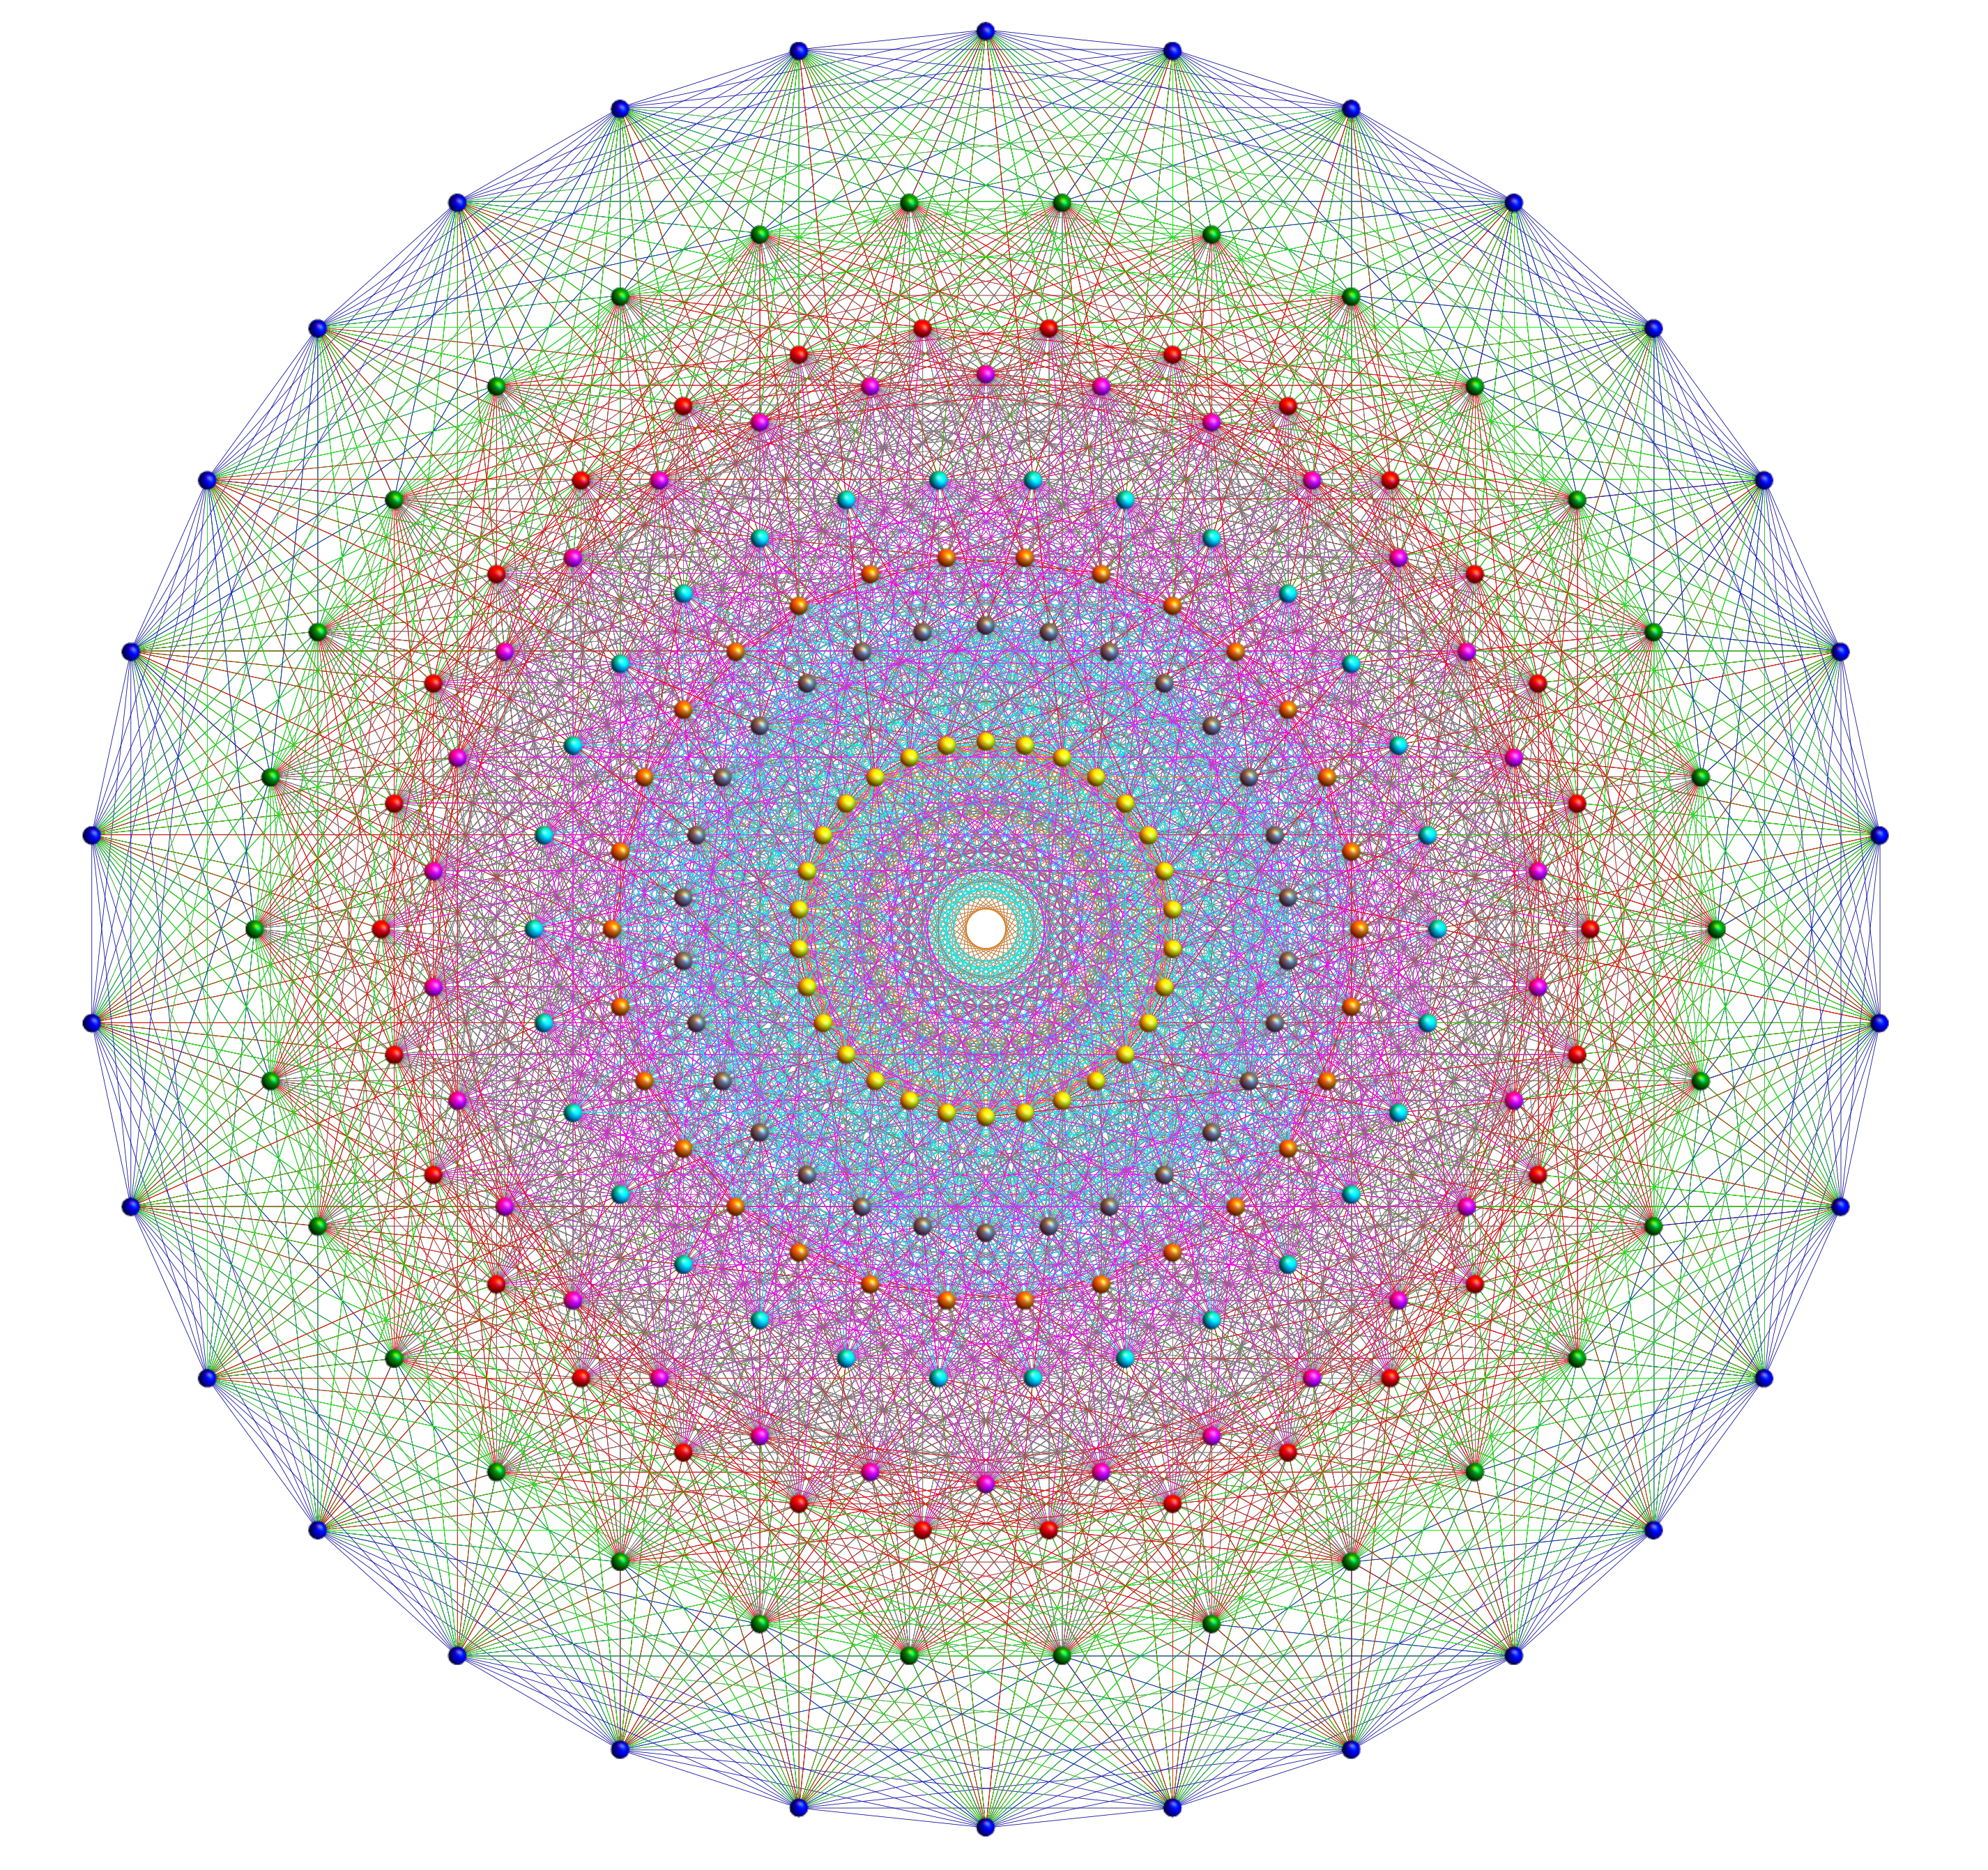
\includegraphics[width=.8\columnwidth]{front.jpeg}
\end{figure}

\newpage
\tableofcontents 
\newpage
\section{Teoria dei gruppi}
\subsection{Il gruppo degli automorfismi}
\begin{lemma}
	Siano $H,G$ due gruppi ciclici; un omomorfismo $\varphi : G \to H$ \`e univocamente determinato da come agisce su un generatore di $G$.
	\begin{proof}
		Sia $g_0\in G$ tale che $\langle g_0 \rangle = G$ e sia $\varphi (g_0) = \overline{h}\in H$.
		Per $g \in G$ generico, per cui $g_0^k = g$ per qualche intero $k$, si ha:
		\[
		\varphi (g) = \varphi (g_0^k) = \varphi (g_0)^k = \overline{h}^k
		\] 
		Cio\`e tutti gli elementi di $\operatorname{Im} \varphi $ sono esprimibili come potenze di $\overline{h}$.
	\end{proof}
\end{lemma}
\begin{osservazione}
Non ogni scelta di $\overline{h} \in H$ \`e ammissibile, ma bisogna rispettare l'ordine di $g_0$.
Se $g_0^n = e_G$, allora $e_H = \varphi (g_0^n) = \varphi (g_0)^n = \overline{h}^n$. Questa condizione, impone che $\operatorname{ord}(\overline{h})  \mid \operatorname{ord}(g_0) $.
\end{osservazione}
\begin{definizione}
	[Gruppo degli automorfismi]
	Sia $G$ un gruppo; si definisce il gruppo dei suoi automorfismi come
	\[
	\operatorname{Aut} (G) = \left\{ f: G \to G  \mid f \text{ \`e un isomorfismo di gruppi} \right\} 
	\] 
\end{definizione}
\begin{esempio}
	Si calcola $\operatorname{Aut} (\mathbb{Z})$. 
	\begin{svolgimento}
		Il gruppo $(\mathbb{Z},+)$ \`e ciclico, quindi un omomorfismo \`e determinato in base a come agisce su un generatore.
		Prendendo, per esempio $1$, si definisce $q_a :\mathbb{Z}\to \mathbb{Z} $ tale che $ q_a (1 ) = a$; perch\'e $\langle q_a(1) \rangle = \mathbb{Z}$\footnote{Richiesto dal fatto che $q_a$ sia suriettivo.}, \`e necessario che $a$ sia un generatore di $\mathbb{Z}$, perci\`o sono ammessi $a = \pm 1$. 
		In questo caso, $\operatorname{Aut} (\mathbb{Z})=\left\{ \pm \operatorname{Id} _{\mathbb{Z}}  \right\} \cong \left(\mathbb{Z} / 2\mathbb{Z}, +\right) $.
	\end{svolgimento}
\end{esempio}
\begin{teorema}
$\operatorname{Aut} (\mathbb{Z} / m \mathbb{Z}) \cong (\mathbb{Z} / m \mathbb{Z})^*$.
\begin{proof}
	$(\mathbb{Z} / m\mathbb{Z}, + )$ \`e ciclico, quindi si stabilisce l'azione di $f:\mathbb{Z} / m\mathbb{Z}\to \mathbb{Z}/ m\mathbb{Z}$ su un generatore.
	Preso, allora, $\overline{k} \in \mathbb{Z} / m\mathbb{Z} $ tale che $\operatorname{gcd}(k,m) =1$ e scelto $f(\overline{k}) = \overline{a}$, si ha che $\langle f(\overline{k}) \rangle= \langle \overline{a} \rangle= \mathbb{Z} / m\mathbb{Z} \iff \operatorname{gcd}(a,m) =1	\iff \overline{a} \in \left(\mathbb{Z} / m\mathbb{Z}\right) ^* $.
\end{proof}
\end{teorema}
\begin{definizione}
	[Automorfismo interno]
	Sia $G$ un gruppo; si definisce $\phi _g :G\to G$, $ \forall g \in G$, come $\phi_g (x) =gxg^{-1} $ ed \`e detto \textit{automorfismo interno}. 
	L'insieme di questi automorfismi, al variare di $g \in G$, forma il gruppo
	\[
	\operatorname{Int} (G) = \left\{ \phi _g : G\to G  \mid g \in G \text{ e } \phi _g \text{ automorfismo interno} \right\} 
	\] 
\end{definizione}
\begin{prop}\label{intcar}
	Sia $G$ un gruppo; allora $\operatorname{Int} (G) \lhd \operatorname{Aut} (G)$ e $\operatorname{Int} (G) \cong G / Z(G)$.
	\begin{proof}
		$\operatorname{Int} (G)$ \`e un sottogruppo di $\operatorname{Aut} (G)$ perch\'e $\operatorname{Id} (x) = exe^{-1} = x  \Rightarrow \operatorname{Id} \in \operatorname{Int} (G)$.
		Inoltre, $\phi _g \circ \phi _h (x) = ghxh^{-1}g^{-1}=\phi _{gh} (x) \in \operatorname{Int} (G)$ e $\phi _{g^{-1} } \circ \phi _g (x) = x \Rightarrow \phi _g^{-1} = \phi _{g^{-1}} \in \operatorname{Int}(G)  $.

		\`E un sottogruppo normale perch\'e $\forall f \in \operatorname{Aut} (G)$, si ha 
		\[
		f \circ \phi _g \circ f^{-1}(x) = f \left(g f^{-1}(x) g^{-1}\right) =f(g) x f(g)^{-1} \in \operatorname{Int} (G)
		\] 
		Per finire, si definisce $\Phi : G \to \operatorname{Int} (G) $.
		Questo \`e un omomorfismo perch\'e $\Phi(gh)=\phi _{gh} = \phi _g\circ \phi _h = \Phi(g)\Phi(h)$.
		\`E, inoltre, suriettivo perch\'e ogni automorfismo interno \`e associato ad un elemento di $G$, cio\`e $\forall \phi _g \in \operatorname{Int} (G), \ \exists g \in G : \Phi(g) = \phi _g$.
		Allora, la tesi deriva dal I teorema di omomorfismo, visto che $\operatorname{Ker} \Phi = Z(G)$.
	\end{proof}
\end{prop}
\begin{osservazione}\label{ossnorm}
	$H \lhd G \iff \phi _g(H) = H, \ \forall \phi _g \in \operatorname{Int} (G)$.
	\begin{proof}
Per ogni elemento di $\operatorname{Int} (G)$, si ha $\phi _g (H) = H \iff gH g^{-1} = H \iff H \lhd G$.
	\end{proof}
	\end{osservazione}
\begin{definizione}
	[Sottogruppo caratteristico]
	Sia $G$ un gruppo e $H < G$. Si dice che $H$ \`e \textit{caratteristico} se \`e invariante per automorfismo, cio\`e $\forall f \in \operatorname{Aut} (G), \ f(H) = H$.
\end{definizione}
\begin{corollario}
	Sia $G$ un gruppo; per la proposizione \ref{intcar} e l'osservazione \ref{ossnorm} se $H$ \`e caratteristico, allora $H \lhd G$.
\end{corollario}
\noindent Il viceversa \`e falso, cio\`e normale $\not\Rightarrow $ caratteristico; infatti, in $\mathbb{Z} / 2\mathbb{Z} \times  \mathbb{Z} / 2\mathbb{Z}$, il sottogruppo $\langle (1,0) \rangle$ \`e normale, ma non caratteristico perch\'e l'automorfismo che scambia le coordinate \`e tale per cui $\langle (1,0) \rangle\mapsto \langle (0,1) \rangle\neq \langle (1,0) \rangle$.
\subsection{Azioni di gruppo}
\begin{definizione}
	[Azione]
	Sia $G$ un gruppo; un'azione di $G$ su un insieme $X$ \`e un omomorfismo
	\[
	\gamma : 
	\begin{array}
		{c c c}
		G &\longrightarrow & S(X) = \left\{ f : X \to X  \mid f \text{ biettiva} \right\} \\
		g & \longmapsto & \psi _g : \psi_g(x) = g \cdot x
	\end{array}
	\] 
Pi\`u concretamente, si definisce \textit{azione} la mappa $\gamma : G \times  X\to X$ tale che
\begin{enumerate}[(a).]
	\item $e\cdot x = x$, per $e \in G$ e $x \in X$;
	\item $h\cdot (g\cdot x) = (hg)\cdot x$, per $g, h\in G$ e $x \in X$.
\end{enumerate}
\end{definizione}
\noindent Si verifica che una mappa $\gamma : G \times  X \to X$, con $G$ gruppo e $X$ insieme generico, che soddisfi le propriet\`a (a) e (b), \`e tale che $\gamma(g) (x) = \psi _g(x)$ (cio\`e a $g$ fissato) \`e biettiva.
\begin{proof}
	Per l'iniettivit\`a, si ha $\psi _g(x) = \psi _g(y) \iff g\cdot x = g\cdot y \iff x = y$, visto che si pu\`o applicare l'azione inversa $\gamma(g^{-1})$ ad entrambi i lati.
	Per la suriettivit\`a, invece, si nota che $\forall x \in X$, si trova anche una $y\in X: y= g^{-1}\cdot x$ dovuta all'azione di $\gamma(g^{-1})$, per cui $\psi _g(y)= g \cdot \left(g^{-1}\cdot x\right) =(gg^{-1}) \cdot x = x$.
\end{proof}
\begin{esempio}
Sia $G = \left\{ z \in \mathbb{C}^*  \mid  \lvert z \rvert =1 \right\} \cong S^1$ la circonferenza unitaria e $X = \mathbb{R}^2$.
Un'azione di $G$ su $X$ \`e una rotazione definita da $\gamma(z) = R(\operatorname{arg} z)$.
Questa \`e un omomorfismo perch\'e $\gamma(zw) = R(\operatorname{arg} zw)  = R(\operatorname{arg} z +  \operatorname{arg} w) = R(\operatorname{arg} z) R(\operatorname{arg} w)= \gamma(z) \gamma(w)$.
\end{esempio}
\noindent Un'azione $\gamma$ di $G$ su $X$ definisce, proprio su $X$, una relazione di equivalenza definita da 
\begin{equation}
	x \sim _\gamma y \iff x=\psi _g(y)=g \cdot y, \text{ con } x,y \in X
\end{equation}
La relazione di equivalenza \`e ben definita perch\'e le $\psi _g$ sono mappe biettive.
\begin{definizione}
	[Orbita]
	Sia $\gamma :G \to S(X)$ un'azione di $G$ gruppo su $X$. Dato $x \in X$, la sua classe di equivalenza rispetto alla relazione $\sim _\gamma$ \`e detta \textit{orbita} ed \`e indicata con $\operatorname{Orb} (x) = \left\{ g \cdot  x  \mid g \in G\right\} $.
\end{definizione}
\noindent Ricordando che una relazione di equivalenza fornisce una partizione dell'insieme su cui \`e definita, si ha:
\begin{equation}
	X = \bigsqcup_{x \in R} \operatorname{Orb} (x)
\end{equation}
con $R$ insieme dei rappresentati di tutte le orbite.
Se, poi, $X$ ha cardinalit\`a finita, allora:
\begin{boxenv}[]
\begin{equation}
	\lvert X \rvert  = \sum_{x \in R}^{} \lvert \operatorname{Orb} (x) \rvert 
\end{equation}
\end{boxenv}
\begin{definizione}
	[Stabilizzatore]
	Sia $\gamma: G \to S(X)$ un'azione di $G$ su $X$; allora per ogni $x \in X$, si definisce l'insieme 
	\[
	\operatorname{Stab} (x) = \left\{ g \in G  \mid g \cdot  x = x \right\} < G 
	\] 	
\end{definizione}
\begin{lemma}\label{l111}
	Sia $G$ un gruppo che agisce su un insieme $X$ e sia $x \in X$ un suo elemento. Dati anche $g\cdot x , h \cdot x \in \operatorname{Orb} (x)$ tali che $g \cdot x = h\cdot x$, allora $g$ e $h$ appartengono alla stessa classe di $G / \operatorname{Stab} (x)$.
\begin{proof}
	Se $g \cdot x, \ h\cdot x \in \operatorname{Orb} (x)$ sono uguali, allora $x =h^{-1} g \cdot x $, cio\`e $h^{-1} g \in G$ lascia invariato $x$, quindi \`e in $\operatorname{Stab} (x)$.
	Da questo segue che $h \operatorname{Stab} (x) = h h^{-1} g \operatorname{Stab} (x) = g \operatorname{Stab} (x)$.
\end{proof}
\end{lemma}
\begin{teorema}[Teorema di orbita-stabilizzatore]\label{osth}
	Esiste una mappa biettiva $\Gamma : \operatorname{Orb} (x) \to G / \operatorname{Stab} (x)$ tale che $\Gamma(g \cdot x) = g \operatorname{Stab} (x)$.
	\begin{proof}
		$\Gamma$ \`e iniettiva come diretta conseguenza del lemma \ref{l111} ed \`e suriettiva perch\'e $\forall g \operatorname{Stab} (x) \in G / \operatorname{Stab} (x), \exists g\cdot x \in \operatorname{Orb} (x)$ tale che $\Gamma(g\cdot x) = g \operatorname{Stab} (x)$.
		Segue che $\lvert \operatorname{Orb} (x)  \rvert = \lvert G \rvert / \lvert \operatorname{Stab} (x) \rvert $.
	\end{proof}
\end{teorema}
\begin{osservazione}
Si osserva che, per il teorema di orbita-stabilizzatore, la cardinalit\`a di un'orbita indica il numero di classi laterali dello stabilizzatore nel gruppo che compie l'azione, cio\`e il teorema di orbita-stabilizzatore si pu\`o riscrivere come $\lvert \operatorname{Orb} (x) \rvert = [G: \operatorname{Stab} (x)] = \lvert G / \operatorname{Stab} (x) \rvert = \lvert G \rvert / \lvert \operatorname{Stab} (x) \rvert $.
\end{osservazione}


\subsubsection{Azione di coniugio}
 Un caso notevole di azione \`e il coniugio: per $X=G$, si definisce $\gamma : G \to \operatorname{Int} (G) \subset S(G)$.
Le orbite indotte da questa azione sono dette \textit{classi di coniugio} e si indicano con $\operatorname{cl} (x)$, mentre lo stabilizzatore \`e detto \textit{centralizzatore} e si indica con:
\begin{equation}
	Z(x) = \left\{ g \in G  \mid g \cdot x = gxg^{-1} = x \right\} 
\end{equation}
Come conseguenza del teorema di orbita-stabilizzatore (\ref{osth}), si ha:
\begin{equation}
	\lvert G \rvert  = \lvert \operatorname{cl} (x)  \rvert  \lvert Z(x) \rvert , \ \forall x \in G
\end{equation}
\begin{prop}
	Sia $G$ un gruppo e $\gamma$ l'azione di coniugio su di esso; allora
	\[
	\bigcap_{x \in G} Z(x) = Z(G)
	\] 
	\begin{proof}
		Si ha $g \in Z(x), \ \forall x \iff gxg^{-1} =x , \ \forall x \in G \iff g \in Z(G)$.
	\end{proof}
\end{prop}
\begin{osservazione}
	[Centro di un sottogruppo]
	Sia $G$ un gruppo e $H < G$; allora il centro di $H$ \`e definito come 
	\[
	\bigcap_{x \in H}  Z(x) = Z(H)
	\] 
\end{osservazione}

\noindent Si considera, ora, l'azione di coniugio di un gruppo $G$ su $X = \left\{ H \subseteq G  \mid H< G \right\} $ e $\gamma(g) = \psi _g$ tale che $\psi_g (H) = gH g^{-1} $. 
Questa \`e un'azione ed \`e ben definita.
\begin{proof}
	Per dimostrare che \`e un'azione, si deve mostrare che la mappa $g \stackrel{\gamma}{\mapsto} \psi _g$ \`e un omomorfismo e che $\psi _g : X \to X$ sia biettiva.

	Si nota che $g \stackrel{\gamma}{\mapsto} \psi _g$ \`e un omomorfismo perch\'e $\psi _{g_1g_2} (H) = g_1g_2Hg_2^{-1}g_1^{-1} = \psi _{g_1} \circ \psi _{g_2} (H)$, cio\`e $g_1g_2\mapsto \psi _{g_1} \psi _{g_2} $.
	Inoltre, $\psi _g:X\to X$ \`e biettiva perch\'e $\exists \psi ^{-1} _g = \psi _{g^{-1}} : \psi _{g^{-1}} \circ \psi _g (H) = H $.

	Per mostrare che \`e ben definita, si fa vedere che effettivamente $\forall g, \psi_g$ mappa un sottogruppo di $G$ in un altro sottogruppo, cio\`e che $gHg^{-1} < G$.
	Intanto, $e \in gHg^{-1} $ perch\'e $H < G \Rightarrow  e \in H \Rightarrow geg^{-1}=e$; poi, $(ghg^{-1})(gh'g^{-1}) = ghh'g^{-1} \in g H g ^{-1}$ e $h^{-1} \in H \Rightarrow \exists (ghg^{-1} )^{-1} = g h^{-1}g^{-1}\in gHg^{-1}$ elemento inverso.
\end{proof}
\noindent Lo stabilizzatore di questa azione \`e detto \textit{normalizzatore}, in quanto \`e definito come tutti elementi di $G$ rispetto a cui $H$ \`e normale: 
\begin{equation}
	N_G(H) = \operatorname{Stab} (H) = \left\{ g \in G  \mid g H g^{-1}= H \right\} 
\end{equation}
Infine, l'orbita \`e l'insieme (classe di equivalenza) di tutti i coniugati di un sottogruppo di $G$:
\begin{equation}
\operatorname{Orb} (H) = \left\{ gHg^{-1}  \mid  g \in G \right\} 
\end{equation}
Per il teorema di orbita-stabilizzatore (\ref{osth}), si ha:
\begin{equation}
	\lvert G \rvert  = \lvert N_G(H) \rvert \lvert \operatorname{Orb} (H) \rvert 
\end{equation}
da cui si ricava anche che $H \lhd G \iff N_G(H) = G \iff \operatorname{Orb} (H) = \left\{ H \right\} $.
\subsubsection{Formula delle classi}

Si ricorda che le orbite definite da un'azione di un gruppo $G$ su un insieme $X$ formano una partizione di $X$ stesso, in quanto sono delle classi di equivalenza.
Se $\lvert X \rvert < \infty$, si ha:
\begin{equation}\label{ossclass}
\lvert X \rvert  = \sum_{x \in R}^{} \lvert \operatorname{Orb} (x) \rvert = \sum_{x \in R}^{} \frac{\lvert G \rvert }{\lvert \operatorname{Stab} (x) \rvert } = \sum_{x \in R'}^{} 1 + \sum_{x \in R \setminus R '}^{} \frac{\lvert G \rvert }{\lvert \operatorname{Stab} (x) \rvert }
\end{equation}
con $R$ insieme dei rappresentanti delle orbite e $R'$ insieme dei rappresentati delle orbite tali che $\operatorname{Orb} (x) = \left\{ x \right\} $, cio\`e degli elementi invarianti sotto l'azione di $G$. 
\begin{teorema}
	[Formula delle classi]
	Sia $\gamma:G \to S(G)$ l'azione di coniugio di un gruppo $G$ su un insieme $X$; allora:
	\begin{equation*}
		\lvert G \rvert  = Z(G) + \sum_{x \in R \setminus Z(G)}^{} \frac{\lvert G \rvert }{\lvert Z(x) \rvert }
	\end{equation*}
	\begin{proof}
		Segue per quanto appena detto e dall'osservazione che
		\[
		R' = \left\{ x \in R  \mid \operatorname{Orb} (x) = x \right\} = \left\{ x \in R  \mid gxg^{-1} = x \right\} = Z(G)
		\] 
		Visto che ogni orbita del genere contiene un solo elemento, i rappresentanti delle orbite sono esattamente tutti gli elementi di $Z(G)$, cio\`e un elemento $x \in Z(G)$ non pu\`o essere contenuto in nessun'altra orbita, se non nel singoletto $\left\{ x \right\} $.
		Perci\`o, la relazione in eq. \ref{ossclass}, avendo $X=G$, conferma la tesi.
	\end{proof}
\end{teorema}
\subsection{I p-gruppi}
\begin{definizione}
	[p-gruppo]
	Sia $p \in \mathbb{Z}$ un numero primo; allora si dice che $G$ \`e $p$-gruppo se $\lvert G \rvert = p^n$, per qualche $n \in \mathbb{N}$.
\end{definizione}
\begin{prop}\label{pnb}
	Il centro di un $p$-gruppo \`e non-banale.
	\begin{proof}
		Per la formula delle classi, si ha:
		\[
		p^n = \lvert Z(G) \rvert  + \sum_{x \in R \setminus Z(G)}^{} \frac{\lvert G \rvert }{\lvert Z(x) \rvert }
		\] 
		Se $\lvert Z(G) \rvert  = p^n$, la tesi \`e verificata, altrimenti $\exists x \in R \setminus Z(G)$, quindi tale che $Z(x) \subsetneq G$; allora, per $k_x\in \mathbb{N}$, si ha $\lvert G \rvert / \lvert Z(x) \rvert = p^{k_x} $, con almeno un $k_x > 0$, da cui:
		\[
		\lvert Z(G) \rvert =p^n - \sum_{x \in R \setminus Z(G)}^{} p^{k_x} \implies p  \mid \lvert Z(G) \rvert 
		\] 
		Visto che $e \in Z(G)$, deve risultare $\lvert Z(G) \rvert \ge 1$, pertanto $\lvert Z(G) \rvert = p^s$, per qualche intero $s > 1$.
	\end{proof}
\end{prop} 
\begin{lemma}\label{GZGciffban}
	Vale $G / Z(G)$ ciclico $\iff G$ \`e abeliano.
	\begin{proof}
		Sia $G / Z(G)$ ciclico e sia $x_0 Z(G)$ il suo generatore.
		Date due classi laterali distinte $xZ(G), yZ(G) \in G / Z(G)$ e visto che $x_0Z(G)$ genera, si avr\`a $x_0^m Z(G)= x Z(G)$ e $x_0^nZ(G) = yZ(G)$, ossia, per $z,w \in Z(G)$, $x = x_0^m z,\ y = x_0^n w$. 
		Allora:
		\[
			 xy = x_0^m z x_0^n w = x_0^m x_0^n zw = x_0^n wx_0^m z = yx
		\] 
	Essendo questo valido per $x,y \in G$ generiche, si \`e dimostrata l'implicazione verso destra.

	Per l'implicazione inversa, sia $G$ abeliano; allora $Z(G) = G$ e $G / Z(G) = \left\{ e \right\} $, che \`e ovviamente ciclico.
	\end{proof}
\end{lemma}
\begin{prop}
	Un gruppo di ordine $p^2$ \`e abeliano.
	\begin{proof}
		Sia $G$ un $p$-gruppo tale che $\lvert G \rvert  = p^2$. Per mostrare che \`e abeliano, si fa vedere che $Z(G) = G$, ossia $\lvert Z(G) \rvert  = p^2$.
		Per la proposizione \ref{pnb}, si pu\`o avere solamente $\lvert Z(G) \rvert = p$, oppure $\lvert Z(G) \rvert = p ^2$.
		Se, per assurdo, fosse $\lvert Z(G) \rvert =p$, allora $\lvert G \rvert / \lvert Z(G) \rvert = p$, quindi $G / Z(G)$ avrebbe ordine primo e, quindi, sarebbe ciclico; per il lemma precedente (\ref{GZGciffban}), per\`o, questo \`e assurdo perch\'e risulterebbe anche abeliano al contempo, ma senza avere $\lvert Z(G) \rvert  = \lvert G \rvert $.
		Quindi deve essere $\lvert Z(G) \rvert  = p^2 = \lvert G \rvert \Rightarrow Z(G) = G$, da cui $G$ \`e abeliano.
	\end{proof}
\end{prop}
\subsection{Teoremi di Cauchy e Cayley}
\begin{lemma}[Teorema di Cauchy abeliano]\label{cab}
	Sia $p$ un primo e $G$ un gruppo abeliano finito; se $p  \mid  |G|$, allora $\exists x \in G : \operatorname{ord}(x) =p$.
	\begin{proof}
		Sia $\lvert G \rvert = pn$; si procede per induzione su $n$.
		Il passo base \`e ovvio: se $\lvert G \rvert =p$, allora \`e ciclico e, quindi, contiene un elemento di ordine $p$.

		Per il passo induttivo, si suppone che la tesi sia vera per ogni $m < n$ e si dimostra per $n$.

		Sia, allora $\lvert G \rvert  = pn$; sia, poi $y \in G, \ y\neq e$ tale che $\langle y \rangle= H < G$: per Lagrange, $\lvert G \rvert  = \lvert G / H \rvert  \lvert H \rvert $.
		Allora, se $p  \mid \lvert G \rvert \Rightarrow  p  \mid \lvert H \rvert $, oppure $ p   \mid \lvert G / H \rvert $.
		\begin{itemize}
			\item Se $p  \mid \lvert H \rvert $, allora pu\`o essere $\lvert G \rvert  = \lvert H \rvert $, caso in cui $G = \langle y \rangle$ sarebbe ciclico e, quindi, avrebbe un elemento di ordine $p$\footnote{In questo caso, l'elemento di ordine $p$ sarebbe proprio $y^{p^{n-1} } \in G $; infatti, $(y^{p^{n-1} } )^p = y^{p^n} = e$, visto che $|G| = p^n$.}, oppure pu\`o essere $\lvert H \rvert  = pm < pn$, caso in cui l'elemento di ordine $p$ \`e presente per ipotesi induttiva.
			\item Se $p  \mid  \lvert G / H \rvert $, invece, allora $\lvert G / H \rvert = pm' < pn$ perch\'e $H$ contiene almeno due elementi, cio\`e $y$ ed $e$; per ipotesi induttiva, allora, esiste $zH \in G / H$ il cui ordine \`e $p$.
				Considerando la proiezione $\pi_H : G \to G / H$ tale che $x \mapsto xH$ e ricordando che \`e un omomorfismo, si ha che, per questo motivo, $\operatorname{ord}(zH)  \mid \operatorname{ord}(z)\Rightarrow \operatorname{ord}(z) = pk$; se $k = n$, allora $G$ \`e ciclico e $z^n$ ha ordine $p$, altrimenti, se $k<n$, si ha la tesi per induzione.
		\end{itemize}
	\end{proof}
\end{lemma}
\begin{teorema}
	[Teorema di Cauchy]
	Sia $p$ un numero primo e $G$ un gruppo finito; se $p  \mid |G|$, allora esiste $x \in G : \operatorname{ord}(x) = p $.
	\begin{proof}
		Sia $|G| = pn$, con $p$ primo e $n \in \mathbb{N}$; si procede per induzione su $n$.
		Se $n=1$, $|G| = p \Rightarrow G$ \`e ciclico, quindi $\exists x \in G : \langle x \rangle=G$ e $\operatorname{ord}(x) = p$.

		Per il passo induttivo, si assume che la tesi sia valida per ogni $ m < n$ e si dimostra per $n$.

Si nota che se $\exists  H < G$ tale che $p  \mid  \lvert H \rvert $, allora $|H|=pm , \ m < n \Rightarrow \exists x \in H$ tale che $\operatorname{ord}(x) =p$ per ipotesi induttiva.
Si assume, dunque, che non esista alcun sottogruppo di $G$ il cui ordine sia divisibile per $p$.
Per la formula delle classi
\[
pn - \sum_{x \in R\setminus Z(G)}^{} \frac{\lvert G \rvert }{|Z(x)|} = \lvert Z(G) \rvert 
\] 
Ora, visto che $Z(x) < G \Rightarrow p$ non divide $|Z(x)|$, quindi si ha la certezza che, essendo $p  \mid |G| = |Z(x)| |G|/|Z(x)|$, $p$ divide $|G|/|Z(x)|$. 
Allora $p  \mid  |Z(G)|$, per cui $Z(G) =G$; infatti, se cos\`i non fosse, sarebbe un sottogruppo proprio di $G$ e $p$ non lo potrebbe dividere, il che \`e assurdo.

Da questo, segue che $G$ \`e abeliano, quindi la tesi segue dal teorema di Cauchy per gruppi abeliani (lemma \ref{cab}).
	\end{proof}
\end{teorema}
\begin{prop}\label{tgen}
Siano $H,K < G$; allora $HK < G \iff HK = KH$ e $\lvert HK \rvert = \lvert H \rvert \lvert K \rvert / \lvert H \cap K \rvert $.
\begin{proof}
Per la prima parte, \`e sufficiente osservare che per $hk \in HK$, l'elemento neutro $(hk)^{-1} = k^{-1} h^{-1} $ sta in $HK$ se e solo se $HK = KH$, e, allo stesso modo, il prodotto \`e chiuso cio\`e $hkh'k' = hh''k''k' \in HK$ solamente se $HK = KH$ cos\`i da poter trovare un elemento di $HK$ che sia uguale a $kh'\in KH$ che compare in tale prodotto.

La seconda parte, invece, si verifica considerando l'applicazione $\gamma: H \times K\to HK$ tale che $\gamma((h,k)) = hk$, che \`e evidentemente suriettiva; inoltre, se $s \in H \cap K$, allora $(hs,s^{-1}k) \in H \times K\Rightarrow \gamma ((hs,s^{-1}k)) = hk$, il che vuol dire che $\forall hk \in HK$, si trovano $|H\cap K|$ coppie in $H \times K$ che hanno immagine $hk$, da cui la tesi.
\end{proof}
\end{prop}
\begin{esempio}[Classificazione dei gruppi di ordine 6]
Sia $G$ un gruppo di ordine $6$; per Cauchy, allora, esistono $x,y \in G$ tali che $\operatorname{ord}(x) = 2$ e $\operatorname{ord}(y) =3$. 
Se $G$ \`e abeliano, poi, si ha $\operatorname{ord}(xy) = 6$\footnote{$\langle x \rangle \cap \langle y \rangle e$ perch\'e sono generati da elementi diversi, altrimenti avrebbero stesso ordine.}, quindi $G = \langle xy \rangle\cong \mathbb{Z}/ 6\mathbb{Z}$.

Se, invece, $G$ non \`e abeliano, si considera il sottogruppo $\langle x,y \rangle$ e si considera anche l'insieme $\langle x \rangle\langle y \rangle$ che, in generale, non \`e un sottogruppo.

Applicando la proposizione precedente (\ref{tgen}), si ha che $\lvert \langle x,y \rangle \rvert = (3 \cdot 2) / 1= 6$\footnote{Come gi\`a accennato, l'intersezione \`e solo l'unit\`a perch\'e i due elementi hanno ordini diversi, quindi generano gruppi disgiunti.}, da cui $G = \langle x \rangle\langle y \rangle$, con $\langle x \rangle= \left\{ e,x \right\} $ e $\langle y \rangle= \left\{ e,y,y^2 \right\} $, quindi $G = \left\{ e , x ,y, xy,y^2 , xy^2 \right\} $.

Per finire, si mostra che $G \cong S_3$. 
Per farlo, si definisce $\phi :G \to S_3=\left\{ e,\tau ,\rho ,\tau \rho ,\tau ^2,\rho \tau ^2 \right\} $ tale che $\phi (x) = \rho $ e $\phi (y) = \tau $, con $\tau =(1,2,3)$ e $\rho = (1,2)$.
Questa mappa \`e suriettiva per costruzione, quindi \`e biettiva per questioni di cardinalit\`a; inoltre, \`e un omomorfismo, da cui segue la tesi.
\end{esempio}

\begin{teorema}
	[Teorema di Cayley]
	Sia $G$ un gruppo; allora $G$ \`e isomorfo a un sottogruppo di $S(G)$.
	In particolare, se $|G| = n$, allora $G$ \`e isomorfo a un sottogruppo di $S_n$.
	\begin{proof}
		Si definisce l'azione
		\[
		\phi : 
		\begin{array}
			{c c c}
			G & \longrightarrow & S(G)\\
			g & \longmapsto & \gamma_g
		\end{array}, \ \text{ tale che } \gamma_g(x) = g\cdot  x=gx
		\] 
		Questa \`e ben definita perch\'e $\gamma:G \to G$ \`e biettiva, infatti $\gamma_g(x) = \gamma_g(y) \iff g x = g y \iff x = y$ e $\forall y \in G , \ \exists \gamma_g(g^{-1} y) = y $, il che mostra che \`e rispettivamente iniettiva e suriettiva.
		Inoltre, $\phi $ \`e un omomorfismo (ovvio) ed \`e anche iniettiva perch\'e $\operatorname{Ker} \phi = \left\{ g \in G  \mid \phi _g = \phi _e \right\} = \left\{ g \in G  \mid g x = x \right\} = \left\{ e \right\}$.
		Da questo, segue che $S(G)$ contiene una copia isomorfa a $G$.
	\end{proof}
\end{teorema}
\subsection{Commutatore e gruppo derivato}


\begin{definizione}
	Sia $G$ un gruppo e $S \subset G$ un suo sottoinsieme; allora $\langle S \rangle$ \`e il pi\`u piccolo sottogruppo di $G$ contenente anche $S$.
\end{definizione}
\begin{prop}
	Dato $G$ un gruppo e $S \subset G$ un suo sottoinsieme, vale la relazione
	\[
	\langle S \rangle= \left\{ s_1s_2 \ldots s_k  \mid k \in \mathbb{N}, \ s_i \in S \cup S^{-1} \right\} = X
	\] 
	con $S^{-1}= \left\{ s^{-1}  \mid  s \in S \right\} $.
	\begin{proof}
		Per definizione
		\[
			\langle S \rangle= \bigcap_{\substack{H < G \\ S \subset H}} H
		\] 
		Questa scrittura \`e ben definita perch\'e l'intersezione di gruppi \`e ancora un gruppo e, in questo modo, si ha il gruppo pi\`u piccolo contenente $S$; se cos\`i non fosse, ne esisterebbe uno pi\`u piccolo ancora, che, per\`o, farebbe parte dell'intersezione e sarebbe assurdo.

		Ora, per quanto detto sopra, $S$ \`e contenuto in tutti i gruppi la cui intersezione genera $\langle S \rangle$, quindi anche $S^{-1} $ deve essere contenuto in tali sottogruppi di $G$.
		Segue che $S,S^{-1}\subset H \Rightarrow X \subset H, \ \forall H < G$ e $S \subset H$, quindi $X \subset \bigcap H = \langle S \rangle$.

		Allo stesso tempo, $X$ \`e evidentemente un sottogruppo di $G$ e contiene $S$ per costruzione, quindi $X \supset \langle S \rangle$, da cui la tesi.
	\end{proof}
\end{prop}
\begin{definizione}
	[Commutatore]
	Sia $G$ un gruppo; dati $g,h \in G$, il loro \textit{commutatore} \`e definito come
	\[
		[g,h] = ghg^{-1} h^{-1}
	\] 
\end{definizione}
\begin{definizione}
	[Gruppo derivato]
	Dato un gruppo $G$, si definisce \textit{gruppo dei commutatori}, o \textit{derivato} di $G$, il gruppo 
	\[
		G ' = \langle [g,h]  \mid g,h \in G \rangle = [G:G]
	\] 
\end{definizione}
\noindent Ora si caratterizza il gruppo derivato.
Intanto, si ricorda che $\langle S \rangle$ \`e abeliano $\iff \forall s_1,s_2\in S , \  s_1s_2=s_2s_1$, $\langle S \rangle$ \`e normale $\iff \forall g \in G, \forall s \in S, \ gsg^{-1} \in \langle S \rangle$ e, infine, $\langle S \rangle$ \`e caratteristico $\iff \forall f \in \operatorname{Aut} (G) ,\ \forall s \in S$ si ha $f(s) \in S$.
Applicando queste alla definizione di commutatore, si ottiene la seguente.
\begin{prop}[Propriet\`a del derivato]\label{propderiv}
	
	Sia $G$ un gruppo e $G'$ il suo derivato; allora:
	\begin{enumerate}[(a).]
		\item $G ' = \left\{ e \right\}  \iff G$ \`e abeliano;
		\item $G' \lhd G$;
		\item $G'$ \`e caratteristico in $G$;
		\item dato $H \lhd G$, se $G / H$ \`e abeliano, allora $G' \subset H$.
	\end{enumerate}
	\begin{proof}
		La (a) \`e immediata perch\'e $G' = \left\{ e \right\} \iff \forall g_1,g_2 \in G, \ [g_1,g_2] = e $, cio\`e $g_1$ e $g_2$ commutano, da cui $G$ abeliano.

		Per la (b), $\forall x \in G, \ \forall g,h \in G $, si ha 
		\[
			\begin{split}
				x[g,h]x^{-1}  &= xghg^{-1}h^{-1}x^{-1}= xgx^{-1}xhx^{-1}xg^{-1}x^{-1}xh^{-1}x^{-1}\\
					      &=[xgx^{-1}, xhx^{-1}] \in G'
			\end{split}
		\] 
	Per la (c), si nota che $\forall f \in \operatorname{Aut} (G), \ \forall g,h \in G$, si ha:
	\[
		f([g,h]) = f(ghg^{-1}h^{-1}) = f(g) f(h) f(g)^{-1} f(h)^{-1} = [f(g), f(h)] \in G'
	\] 
	Infine, per la (d), se $H \lhd G$ e $G / H$ \`e abeliano, si ha $\forall x,y \in G$
	\[
		xHyH =yH xH\Rightarrow xyH = yxH \implies x^{-1}y^{-1}xy \in H \Rightarrow [x,y] \in H
	\] 
	da cui $H \supset G' $.
	\end{proof}
\end{prop}
\begin{corollario}
	Sia $G$ un gruppo e $G'$ il suo derivato; allora $G / G'$ \`e sempre abeliano ed \`e chiamato \textit{abelianizzazione} di $G$, nel senso che \`e il pi\`u grande quoziente abeliano di $G$.
	\begin{proof}
		Si mostra che $G / G'$ \`e sempre abeliano. 
		Siano, quindi $gG', hG' \in G / G'$ due classi laterali; allora si osserva che
		\[
			(gG') (hG') = ghG' = hg [g^{-1},h^{-1}] G' = hg G'
		\] 
		visto che $g^{-1}h^{-1}gh=[g^{-1},h^{-1}] \in G'$.
		Allora, dalla propriet\`a (d) della precedente proposizione (\ref{propderiv}), si ha $G' \subset H =G'$, cio\`e in questo caso si ha l'inclusione nell'insieme pi\`u piccolo, ovvero proprio $G'$. 
		Questo vuol dire che $G /G'$ \`e il quoziente con pi\`u elementi che sia abeliano perch\'e ottenuto tramite quoziente con $G'$, che \`e l'insieme pi\`u piccolo che soddisfa la propriet\`a\footnote{Per controposizione, se $G'\not\subset H\implies G/H$ non abeliano.}.
	\end{proof}
\end{corollario}
\subsection{Gruppi liberi}
Si definisce l'insieme $S=\left\{ x_1,x_2,x_3,\ldots \right\} $ di simboli arbitrari, che pu\`o essere finito o infinito, e si definisce \textit{parola} una qualunque loro concatenazione, in cui sono ammesse ripetizioni. 
L'insieme delle parole ottenibili a partire dagli elementi di $S$ si indica con $W $.
Le concatenazioni dello stesso simbolo si possono esprimere in notazione esponenziale: $x_1 x_1 \ldots x_1 = x_1^n$.

Per arrivare alla costruzione di un gruppo, servono degli inversi ed un elemento neutro; l'elemento neutro si indica con $1$ ed \`e tale per cui
\[
1 \cdot \prod_{i} x_i^{a_i} = \prod_{i} x_i^{a_i} \cdot 1 = \prod_{i} x_i^{a_i} 
\] 
L'insieme degli elementi inversi, invece, si indica con $S^{-1}$ e si definisce $S' = S \cup S^{-1}$.
Indicando, ora, con $W'$ l'insieme delle parole che si possono costruire in $S'$, si nota la possibilit\`a di trovare una sequenza della forma $\ldots x x^{-1}\ldots$, oppure $\ldots x^{-1}x \ldots$; questo indica che la parola pu\`o essere opportunamente ridotta cancellando tali simboli, cio\`e usando la definizione $x^{-1} x = x x^{-1}= 1$.
\begin{definizione}
	[Parola ridotta]
	Una parola di $W'$ si dice \textit{ridotta} se non \`e possibile operare ulteriori cancellazioni.
\end{definizione}
\noindent A partire da una stessa parola, o dalle sue cancellazioni, \`e possibile operare la riduzione cancellando i termini in ordine diverso, ma giungendo sempre allo stesso risultato.
Alla luce di questo, si ha la seguente definizione.
\begin{definizione}
	[Parole equivalenti]
	Due parole $w, w' \in W'$ si dicono \textit{equivalenti}, e si scrive $w \sim w'$, se hanno la stessa forma ridotta $w_0$.
\end{definizione}
\begin{osservazione}
	Si pu\`o dimostrare che $\sim$ \`e una relazione di equivalenza.
\end{osservazione}
\begin{prop}
	Sia $F$ l'insieme delle classi di equivalenza di parole in $W'$; allora $F$ \`e un gruppo rispetto alla legge di composizione indotta $W'$.
	\begin{proof}
		La concatenazione di parole di $W'$ \`e associativa e la legge di composizione indotta da questa tra le parole che rappresentano una classe di equivalenza sar\`a altrettanto associativa.
		Inoltre, la classe dell'elemento neutro $1$ \`e l'identit\`a e la classe della parola inversa di $w$ \`e l'inversa della classe di $w$.
	\end{proof}
\end{prop}
\begin{definizione}
	[Gruppo libero]
	Si definisce \textit{gruppo libero sull'insieme} $S$ il gruppo $F$ con la composizione indotta da $W'$.
\end{definizione}
\noindent Si indica con $F_1$ il gruppo libero su $S = \left\{ x \right\} $, cio\`e \`e il gruppo generato da un singolo simbolo e da tutte le sue concatenazioni, quindi da tutte le sue potenze.
Questo si sa caratterizzare bene perch\'e, evidentemente, $F_1 \cong \mathbb{Z}$; infatti basta definire $\phi :\mathbb{Z}\to F_1$, con $\phi (k) = x^k$.

\begin{prop}
	[Propriet\`a universale]
	Sia $F_S$ il gruppo libero su un insieme $S$ e sia $G$ un gruppo; ogni applicazione tra insiemi $f: S \to G$ si estende in modo unico ad un omomorfismo di gruppi $\varphi : F_S \to G$.
	\begin{proof} 
Indicando con $\widetilde{x}=f(x)$, per $x \in S$, allora $\varphi $ mappa una parola di $S'$ nel corrispondente prodotto in $G$.

Si nota che $f$ associa un simbolo ad un elemento di $G$; allora la mappa $\varphi $ associa, a ciascuna parola composta dai simboli di $S'$, la loro immagine tramite $f$: se $w = x_1 \cdots x_n$, allora $\varphi (w) = f(x_1) \ldots f(x_n)=\widetilde{x}_1 \cdots \widetilde{x}_n$, con $\varphi (x^{-1})=f(x)^{-1} = \widetilde{x}^{-1}$.

Due parole equivalenti di $S'$, allora, vengono mappate nell'analogo prodotto in $G$, per cui risulteranno avere stessa immagine attraverso $\varphi $; questo perch\'e se $w$ e $w'$ si riducono a $w_0$, allora la loro immagine tramite $\varphi $ andr\`a in due elementi il cui prodotto si ridurr\`a al prodotto degli elementi immagine di $w_0$.

Infine:
\[
w w'=x_1\cdots x_n x'_1\cdots x'_n\longmapsto \widetilde{x}_1 \cdots \widetilde{x}_n \widetilde{x}'_1 \cdots \widetilde{x}'_n= \varphi (w)\varphi (w')
\] 
il che prova che $\varphi $ \`e un omomorfismo.
L'unicit\`a deriva dal fatto che $\varphi $ \`e univocamente determinato da come $f$ mappa gli elementi di $S$ in quelli di $G$; se, infatti, si avesse $\varphi (w) = \varphi (w')$, allora si avrebbe $f(x_i) = f(x'_i), \ \forall i$.
	\end{proof}
\end{prop}
\begin{prop}
	[Presentazione di un gruppo]
	Sia $G$ un gruppo generato da $n$ elementi $g_1,\ldots,g_n$ e sia $F_n$ il gruppo libero su un insieme di $n$ elementi; allora $F_n / \operatorname{Ker} \varphi  \cong G$, con $F_n \stackrel{\varphi }{\longrightarrow} G$.
	\begin{proof}
		Per la precedente proposizione, esiste un omomorfismo $\varphi : F_n \to G$ tale che a ciascun $x_i \in F_n$ \`e associato il relativo generatore $g_i \in G$; visto che $\left\{ g_1,\ldots,g_n \right\} \subset \operatorname{Im} \varphi < G$, allora $\operatorname{Im} \varphi = G$, essendo che $\operatorname{Im} \varphi $ contiene tutti i generatori di $G$ ed ogni loro potenza.
		Per il I teorema di omomorfismo, allora, $F_n / \operatorname{Ker} \varphi \cong G$.
	\end{proof}
\end{prop}
\begin{osservazione}
Il nucleo dell'omomorfismo $\varphi $ definito sopra \`e composto da tutte quelle relazioni che mappano i generatori nell'elemento neutro.

In realt\`a, il nucleo \`e il pi\`u piccolo sottogruppo normale ottenuto a partire dall'insieme delle relazioni, indicato con $\langle R \rangle_N$.
Questo significa che se una relazione del tipo $r = 1$ vale in $G$, allora vale anche $xrx^{-1}=1$, visto che $\langle R \rangle_N$ \`e normale per definizione e, quindi, contiene tutti i suoi coniugati.
\end{osservazione}
\begin{esempio}
Si ha $\mathbb{Z} / n\mathbb{Z} = \langle x  \mid (x,n) = 1 \text{ e } x^n = 0 \rangle\cong F_1 / \langle x^n \rangle$.
\end{esempio}
\begin{prop}
	[Presentazione dei gruppi quoziente]
	Sia $G$ un gruppo e sia $N \lhd G$. 
	Si considera $G / N$, ottenuto tramite la proiezione $\pi : G \to G / N$, con $\pi(x) = \overline{x}=x N$, e si considera, dato un altro gruppo $G'$, $\varphi :G \to G'$ un omomorfismo tale che con $N < \operatorname{Ker} \varphi $; allora $\exists ! \overline{\varphi }: G / N \to G '$ tale che $\overline{\varphi }\circ \pi = \varphi $.
\begin{proof}
	Si dimostra che \`e soddisfatto il seguente diagramma:
	\[
	\begin{tikzcd}
		G & & G '\\
		\\
		\\
		 G / N
		\arrow[from=1-1, to=1-3, "\displaystyle \varphi "]
		\arrow[from=1-1, to=4-1, "\displaystyle \pi"']
		\arrow[from=4-1, to=1-3, "\displaystyle \overline{\varphi}"']
	\end{tikzcd}
	\] 
	con $\overline{\varphi }(\overline{a}) = \varphi (a)$.

	Per poter definire $\overline{\varphi } : G / N \to G$, bisogna definire $\overline{\varphi }(\alpha ), \ \forall \alpha \in G / N$; per farlo, si sceglie $a \in G : \pi (a) = \alpha $, per cui $\alpha  = \overline{a}$. 
	Volendo che $\overline{\varphi }(\pi(a)) = \varphi (a)$, si deve definire $\overline{\varphi }$ tramite la relazione $\overline{\varphi }(\alpha ) = \varphi (a)$.

	Ora si fa vedere che, in questo modo, $\overline{\varphi }$ \`e ben definito, cio\`e si mostra che il valore $\overline{\varphi }(\alpha )$, cio\`e $\varphi (a)$, non dipende dalla scelta del rappresentante della classe di equivalenza.
	Siano, allora, $a,a' \in G : \overline{a}= \overline{a}' = \alpha $; l'uguaglianza $\overline{a}=\overline{a}'$ implica che $a' = an$, per qualche $n \in N$ e, visto che $N\subset\operatorname{Ker} \varphi $, si ha $\varphi (a')=\varphi (a)\varphi (n)=\varphi (a)$.

	Per finire, si ha che $\overline{\varphi }$ \`e un omomorfismo perch\'e $\overline{\varphi }(\overline{a})\overline{\varphi }(\overline{b}) = \varphi (a)\varphi (b) = \varphi (ab) = \overline{\varphi }(\overline{ab})$, mentre l'unicit\`a deriva dal fatto che, se $\exists \overline{\psi }$ tale che $\varphi = \overline{\psi }\circ\pi$, allora $\overline{\psi }(\alpha ) = \overline{\psi }(\pi(a)) = \varphi (a) = \overline{\varphi }(\pi(a))=\overline{\varphi }(\alpha ), \ \forall \alpha $.
\end{proof}
\end{prop}
\begin{teorema}\label{mitoat}
	Siano $H, K$ due gruppi, con $H = \langle x_1,\ldots,x_n  \mid R \rangle$, cio\`e \`e generato dagli $x_i$, i quali soddisfano anche le relazioni $R=\left\{ w_1,\ldots,w_m \right\} $; allora:
	\[
		\mathrm{Hom} (H,K) \longleftrightarrow
			\left\{ \left\{ x_1,\ldots,x_n \right\} \stackrel{f}{\longrightarrow} K \ \Big\lvert\ f(x_1),\ldots,f(x_n)\text{ soddisfano le relazioni di } R \right\} 
	\] 
	dove la doppia freccia indica una biezione.
	\begin{proof}
Sia \(F=\langle x_1,\dots,x_n\rangle\) il gruppo libero sui generatori \(x_1,\dots,x_n\) e sia \(N\) la chiusura normale di \(R\) in \(F\); allora, per la presentazione dei gruppi quoziente, si ha $F / N \cong H$. 
Sia, ora:
\[
\Phi:\operatorname{Hom}(H,K)\longrightarrow \{(k_1,\dots,k_n)\in K^n:\ k_i=f(x_i)\text{ soddisfano }R\}
\]
che mappa ciascun omomorfismo $f \in \mathrm{Hom} (H,K)$ nella $n$-upla \((f(x_1),\dots,f(x_n)) \in K^n\).

\begin{enumerate}[(a).]
	\item $\Phi$ \`e ben definita.

Se $f \in \mathrm{Hom} (H,K)$, allora ogni parola \(w\in R\) rappresenta l'identità in \(H\), quindi la sua immagine tramite \(f\) è l'identità in \(K\). 
Pertanto le componenti \(f(x_i)\) soddisfano le relazioni di \(R\).

\item $\Phi$ \`e iniettiva.

Siano \(f,g \in \mathrm{Hom} (H,K)\) tali che \(\Phi(f)=\Phi(g)\); allora \(\forall i, f(x_i)=g(x_i)\).
Visto che gli \(x_i\) generano \(H\), allora ogni elemento di \(H\) è una parola nei generatori; dato che \(f\) e \(g\) coincidono sui generatori, ne segue che coincidono su tutto \(H\), quindi \(f=g\).

\item $\Phi$ \`e suriettiva.

Sia \((k_1,\dots,k_n)\in K^n\) una \(n\)-upla che soddisfa le relazioni di \(R\); allora esiste un unico omomorfismo $f : F \to K$ che manda \(x_i\longmapsto k_i\).
Le ipotesi sulle relazioni implicano che ogni \(w\in R\) viene mandata nell'identità di \(K\), cioè $N < \operatorname{Ker} f$; per la presentazione dei gruppi quoziente, allora, si ha $\overline{f}:F / N \cong H \longrightarrow K$ che mappa la classe di $x_i$ in $k_i$.
Quindi la $n$-upla data è l'immagine di $\overline{f}$ tramite \(\Phi\).
\end{enumerate}
Se ne conclude che \(\Phi\) è una biezione, quindi esiste una corrispondenza biunivoca tra gli omomorfismi \(H\to K\) e le \(n\)-uple di elementi di \(K\) che soddisfano le relazioni \(R\). 
\end{proof}
\end{teorema}
\begin{osservazione}
Si nota che nella formulazione del teorema si può usare indifferentemente l'insieme delle funzioni \(f:\{x_1,\dots,x_n\}\longrightarrow K\), che mappano \(x_i\) in elementi di \(K\) che soddisfano \(R\), oppure l'insieme delle \(n\)-uple \(\{(k_1,\dots,k_n)\in K^n:k_i \text{ soddisfano } R\}\).
Questo perché, fissato l'ordinamento dei generatori \(x_1,\dots,x_n\), esiste una biezione 
\[
\left\{ f:\{x_1,\dots,x_n\}\longrightarrow  K\right\}\xrightarrow{\ \cong\ }K^n,\qquad f\longmapsto\big(f(x_1),\dots,f(x_n)\big)
\]
\end{osservazione}

\subsection{Gruppi diedrali}
\begin{definizione}
	[Gruppo diedrale]
	Per $n \in \mathbb{N}$, si considera un $n$-agono regolare nel piano; l'insieme di tutte le isometrie del piano che mandano l'$n$-agono in se stesso \`e indicato con $D_n$ ed \`e noto col nome di \textit{gruppo diedrale}.
\end{definizione}
\begin{prop}
	Per $n \in \mathbb{N}$, il gruppo diedrale $D_n$ ha cardinalit\`a $\lvert D_n \rvert = 2n$.
	\begin{proof}
		Un'isometria \`e univocamente determinata dall'immagine di un vertice e di un lato adiacente al vertice stesso; allora, l'immagine pu\`o essere pari a $n$ possibili vertici, con due, conseguenti, possibilit\`a per il lato, da cui $2n$ possibili isometrie.
	\end{proof}
\end{prop}
\begin{prop}
	Sia $\rho $ una rotazione che sottende un lato\footnote{Cioè che manda un lato nel successivo.} e $\sigma $ una simmetria (riflessione) dell'$n$-agono regolare; allora $\rho ^n = e$, $\sigma ^2 =e$ e $\sigma \rho \sigma = \rho ^{-1} $.
	\begin{proof}
		Visto che $\rho $ manda un lato dell'$n$-agono regolare nella posizione del successivo, impiegher\`a $n$ iterazioni a far tornare il lato di partenza nella posizione originale; similmente, se $\sigma $ \`e una riflessione, sar\`a sufficiente riapplicarla per far tornare l'$n$-agono nella posizione originale.

		Per l'ultima, si nota che, componendo una rotazione e una riflessione, si ottiene una riflessione; applicando la seconda propriet\`a, si ottiene $\sigma \rho \sigma \rho = e \Rightarrow \sigma \rho \sigma  = \rho ^{-1} $.
	\end{proof}
\end{prop}
\begin{osservazione}
	Ponendo l'$n$-agono regolare nel piano $\mathbb{R}^2$, gli elementi di $D_n$ si possono mettere in relazione con $\mathrm{GL} _2(\mathbb{R})$, visto che si possono vedere come applicazioni lineari da $\mathbb{R}^2$ in se stesso, cio\`e possono essere rappresentate tramite matrici\footnote{Le riflessioni cos\`i definite devono essere rispetto ad un asse opportuno, cio\`e che sia un asse di simmetria per l'$n$-agono in questione. Nella matrice delle riflessioni, l'angolo $\theta $ \`e l'angolo dell'asse rispetto a cui si riflette ed \`e preso con riferimento all'asse $x$.}:
\begin{equation*}
	\rho  \stackrel{\gamma}{\longmapsto} \begin{pmatrix} \displaystyle \cos \left(2k\pi / n\right) & \sin \left(2k\pi / n\right) \\ - \sin \left( 2k\pi / n\right) & \cos (2k\pi / n) \end{pmatrix}=M_\rho  \hspace{1cm}\sigma \stackrel{\gamma}{\longmapsto} \begin{pmatrix} \cos 2 \theta  & \sin 2\theta  \\ \sin 2\theta  & - \cos 2\theta  \end{pmatrix} = M_\sigma 
\end{equation*}
Si nota, inoltre, che indicando con $\mathbb{D}_n$ il gruppo generato da queste matrici, allora la mappa $\gamma : \langle \rho ,\sigma  \rangle\to \mathbb{D}_n$ \`e un omomorfismo di gruppi; infatti, dati due elementi $s_1,s_2 \in \langle \rho ,\sigma  \rangle$:
\[
\gamma(s_1s_2)v= M_{s_1s_2} v = (s_1s_2) (v) = s_1 (s_2 (v)) =M_{s_1} M_{s_2} v = \gamma(s_1)\gamma(s_2)v
\] 
con $v \in \mathbb{R}^2$ e $s(v)$ \`e l'applicazione della rotazione o riflessione $s \in \langle \rho ,\sigma  \rangle$ a tale vettore di $\mathbb{R}^2$.
Conseguentemente, si ha $M_\rho ^n = \operatorname{Id}=M_\sigma ^2 $ e $M_\sigma M_\rho M_\sigma = M_\rho ^{-1}$.

Essendo $\gamma$ un omomorfismo, si vede anche che $\rho $ e $\sigma $, come elementi di $D_n$, non sono legati da alcuna relazione perch\'e, altrimenti, lo sarebbero anche le loro matrici associate, cosa che sarebbe assurda. 
\end{osservazione}
\begin{prop}\label{dnitems}
	Tutti gli elementi di $D_n$ si scrivono come $\sigma \rho ^i$, oppure $\rho ^i$, con $i \in \left\{ 0,\ldots,n-1 \right\} $.
	\begin{proof}
	Sia $g \in D_n$; allora $g$ sar\`a una generica composizione di riflessioni e rotazioni del tipo $g= \rho ^{a_1} \sigma ^{b_1} \ldots \rho ^{a_k} \sigma ^{b_k} $, dove $a_i \in \mathbb{Z}$ e $b_j \in \left\{ 0,1 \right\} $. 
	Usando le relazioni $\sigma ^2 = \rho ^n = e$, si riscalano gli esponenti per scrivere $g = \rho ^{c_1} \sigma \ldots \rho ^{c_m} \sigma $, dove si sono anche, eventualmente, uniti esponenti di rotazioni consecutive (quindi $m\le k$).
	Ora, utilizzando la relazione $\rho \sigma =\sigma \rho ^{-1}$, \`e possibile spostare tutte le $\sigma$ verso l'estrema sinistra, cio\`e come primo termine della parola; cos\`i facendo, si vede che tale parola diventa o una potenza di $\rho $, oppure un termine del tipo $\sigma \rho ^d$, che \`e esattamente quello che si voleva dimostrare.
			\end{proof}
\end{prop}
\noindent Grazie alla precedente proposizione, \`e possibile definire $\rho ^{[i]} = \rho ^i$, con $[i] \in \mathbb{Z} / n\mathbb{Z}$, visto che $\rho ^n = e$.

Inoltre, se $\rho ,\sigma  \in D_n$, allora $\langle \rho ,\sigma  \rangle< D_n$; per\`o, per quanto detto finora, si ha $\lvert \langle \rho ,\sigma  \rangle \rvert = 2n$ perch\'e $\rho ^n = e= \sigma ^2 $, quindi, per ragioni di cardinalit\`a, segue che $D_n = \langle \rho ,\sigma  \rangle$.

\subsubsection{Sottogruppi di $D_n$}
\hfill

\textbf{Numero di elementi di ordine k.} 
Sia $\rho $ una rotazione in $D_n$; si considera $\langle \rho  \rangle\cong C_n < D_n$\footnote{Qui, con $C_n$ si indica un generico gruppo ciclico di ordine $n$.}.

Essendo $C_n$ ciclico, vi sono $\phi (k)$ elementi di ordine $k$, se $k  \mid  n$.
Oltre alle $n$ rotazioni $\rho ^i$, in $D_n$ sono presenti anche le $n$ riflessioni $\sigma \rho ^i$; osservando che $\sigma \rho ^i \sigma \rho ^i = \rho ^{-i}\rho ^{i} = e $, si conclude che se $n$ \`e pari, vi sono $n+1$ elementi di ordine $2$ (cio\`e le $n$ riflessioni e $\rho ^{n / 2} $), mentre se $n$ \`e dispari, vi sono $n$ elementi di ordine $2$.
Ricapitolando:
\begin{equation}
\# \left\{ \text{elementi di ordine } k \right\} = \begin{cases}
	n + 1 &,\ \text{ se } k=2 \text{ e } n \text{ pari}\\
	n  &,\  \text{ se }k=2 \text{ e } n \text{ dispari}\\
	\phi (k)&,\ \text{ se } k \mid n\\
	0 &,\ \text{ altrimenti }
\end{cases}
\end{equation}
visto che le $n$ riflessioni sono tutte di ordine $2$ e l'esistenza di $\rho ^{n / 2} $ dipende dalla parit\`a di $n$.
\vspace*{5pt}

 \textbf{I sottogruppi.} 
Nel punto precedente, si \`e notato che $C_n$ \`e uno dei sottogruppi.
Inoltre, i sottogruppi di $C_n$ sono noti: ne esiste uno per ogni divisore dell'ordine del gruppo, cio\`e $n$ in questo caso, per cui se $H < D_n$ e $H < C_n$, allora $H$ \`e l'unico sottogruppo di ordine $\lvert H \rvert $.
Se, invece $H< D_n$ e $H \not < C_n$, allora $H$ contiene almeno una riflessione $\tau $.
\begin{prop}
	Per $H < D_n$ e $H\cap C_n \neq H$ (cio\`e $H$ contiene almeno una riflessione), si ha $H=(H \cap C_n) \bigsqcup (\tau H \cap C_n) $ ed esiste una mappa biettiva tra $(H\cap C_n)$ e $(\tau H\cap C_n)$\footnote{Per $\tau H\cap C_n$, si intende $\tau (H\cap C_n)$.}.
	\begin{proof}
		Si considera 
	\[
\begin{tikzcd}
H \arrow[r, "\gamma"] 
    \arrow[rr, bend right=30, "{\varphi }"'] & 
\mathrm{GL}_2(\mathbb{R}) \arrow[r, "\det"] & \{\pm 1\}\cong \mathbb{Z}/2\mathbb{Z}
\end{tikzcd}
\]
dove $\gamma$ \`e l'omomorfismo che a $\rho $ e $\sigma $ associa le relative matrici, mentre le matrici di $\mathrm{GL} _2(\mathbb{R})$ sono mappate a $\left\{ \pm 1 \right\} $ tramite il determinante: $\det M_\rho  = 1$ e $\det M_\sigma = -1$.
La mappa $\varphi = \gamma\circ \det$ \`e un omomorfismo suriettivo, infatti $\gamma$ \`e un omomorfismo e per il teorema di Binet per cui $\det (M^i_\rho M^j_\sigma ) = \det(M_\rho )^i \det (M_\sigma )^j = 1 ^i (-1)^j = 1 \iff j= 0$. 
La suriettivit\`a \`e assicurata dal fatto che almeno una riflessione stia in $H$.

Considerando, quindi, $\varphi  :H \to \mathbb{Z} / 2\mathbb{Z}$, il suo kernel \`e $H\cap C_n$; per il I teorema di omomorfismo, allora, $H / (H\cap C_n) \cong \mathbb{Z} / 2\mathbb{Z}$, da cui $\lvert H \rvert / \lvert H\cap C_n \rvert = \lvert \mathbb{Z} / 2 \mathbb{Z} \rvert =2$.

Poi, $\tau H \cap C_n$ e $ H \cap C_n$ sono disgiunti perch\'e se $h \in H\cap C_n$ non potrebbe stare anche in $\tau H\cap C_n$, altrimenti sarebbe una rotazione e una riflessione allo stesso tempo.

Rimane da mostrare solo che i due insiemi hanno stessa cardinalit\`a, quindi l'esistenza di una mappa biettiva che li colleghi.
Sia, allora
\[
\psi  : 
\begin{array}
	{c c c}
	H \cap C_n & \longrightarrow  & \tau  H \cap C_n\\
	h & \longmapsto &\tau  h
\end{array}
\] 
questa \`e biettiva perch\'e $\tau h_1=\tau h_2 \iff h_1=h_2$ e $\forall \tau h\in \tau H \cap C_n$, si ha $\psi (h)=\tau h $.
\end{proof}
\end{prop}
\noindent Si osserva che, per qualche $m$, $H \cap C_n = \langle \rho ^m \rangle= \left\{ e ,\rho ^m , \rho ^{2m} ,\ldots,\rho ^{n - m}  \right\} $, con $m  \mid  n$; se $\tau  = \sigma  \rho ^i $, allora $\tau  H \cap C_n = \left\{ \sigma \rho ^i, \sigma \rho ^{i+m}, \ldots, \sigma \rho ^{i+n - m}   \right\}$ e si sa che l'unione dei due restituisce tutto $H$.
Allora $H$ \`e composto da $m$ rotazioni e $m$ simmetrie; in particolare $H = \langle \rho ^m , \tau  \rangle\cong D_m$, quindi, se $m  \mid  n$, si hanno dei sottogruppi della forma $\mathbb{Z} / m \mathbb{Z}$ e $D_m$.
\vspace{5pt}

\textbf{Sottogruppi normali.} Per lo studio dei sottogruppi normali, si considerano le due seguenti proposizioni.
\begin{prop}
	Sia $H<G$ un sottogruppo tale che $[G:H] = 2$; allora $H\lhd G$.
	\begin{proof}
		Si considerano gli insiemi $\left\{ H,gH \right\} $ e $\left\{ H,Hg \right\} $ delle classi laterali, rispettivamente, sinistre e destre di $H$ in $G$, con $g\not\in H$.
		Ora, $\forall x \in H$, si ha direttamente $xH=H=Hx$; si mostra che lo stesso vale anche per elementi non in $H$.
		Se $y \in G \setminus H$, allora $yH\neq H \neq Hy$; visto che entrambe le classi laterali formano una partizione di $G$, allora deve valere $yH = G \setminus H = Hy$, pertanto $yH=Hy, \ \forall y \in G \setminus H$.
		Si conclude che $gH=Hg, \ \forall g \in G$, quindi $H\lhd G$.
	\end{proof}
\end{prop}
\begin{prop}
	Siano $H \lhd G$ e $K < H$, con $K$ caratteristico in $H$; allora $K \lhd G$.
	\begin{proof}
		Si considera, per $g \in G$, $\phi _g : G\to G$ con $\phi_g(x) = gxg^{-1}$; per definizione, si ha $\phi _g (H) = H$, quindi $\phi_g|_{H} $ \`e un automorfismo e, allora, $\phi _g|_{H} (K) = K, \ \forall g \in G \Rightarrow gKg^{-1} = K$, pertanto $K \lhd G$.
	\end{proof}
\end{prop} 

\noindent L'indice di $C_n$ in $D_n$ \`e $2$, quindi $C_n \lhd D_n$ per la prima proposizione.
Per $G$ ciclico di ordine $n$, esiste un unico $H $, con $\lvert H \rvert =m  \mid n$; visto che ogni sottogruppo di un gruppo ciclico \`e caratteristico, allora, nel caso di $D_n$, ogni sottogruppo di $\langle \rho  \rangle\cong C_n$ \`e caratteristico, quindi normale.

Se $n$ \`e pari, allora $\langle \rho ^2  \rangle<C_n$ ha $n / 2$ elementi; considerando $H < D_n$ e $H \not \subset C_n$, con $H\cap C_n = \langle \rho ^2 \rangle$, si ha
\[
H=\langle \rho ^2 \rangle \sqcup \tau  \langle \rho ^2 \rangle
\] 
quindi $[D_n : H] = 2$, per cui $H \lhd D_n$.
Di sottogruppi di questa forma, se ne trovano due: $\langle \rho ^2 , \sigma  \rangle$ e $\langle \rho ^2 , \sigma \rho  \rangle$; tuttavia non si sa se siano tutti i sottogruppi normali, quindi si cerca di caratterizzarli meglio.

Si sa che $H \lhd G \iff gHg^{-1}= H , \ \forall g \in G$, quindi per ogni elemento di un sottogruppo normale, devono figurare anche tutti i suoi coniugati.
Per la proposizione \ref{dnitems}, per capire come sono fatti i coniugati di $D_n$, \`e sufficiente studiare quali siano quelli di $\rho ^i$ e $\sigma \rho ^i$. 
Si nota che:
\[
	\rho ^j \rho ^i \rho ^{-j}= \rho ^i \hspace{1cm}\sigma \rho ^j \rho ^i \rho ^{-j}\sigma  = \sigma \rho ^i\sigma =\rho ^{-i}
\] 
quindi l'insieme dei coniugati di $\rho ^i$ \`e $\left\{ \rho ^i, \rho ^{-i} \right\} $; in particolare, se $i \in \left\{ 0 , n /2 \right\} $, tale insieme diventa $\left\{ e \right\} $, oppure $\left\{ \rho ^{ n / 2}  \right\} $ rispettivamente.
Poi, si nota che:
\[
\rho ^i \sigma \rho ^j \rho ^{-i}= \sigma \rho ^{-i}\rho ^j\rho ^{-i}=\sigma \rho ^{j-2i} \hspace{1cm} \sigma \rho ^i\sigma \rho ^j \rho ^{-i} \sigma = \rho ^{-i}\rho ^j\rho ^{-i}\sigma =\sigma \rho ^{2i-j} 
\] 
quindi se $n$ \`e pari, allora $\sigma \rho ^s \sim \sigma \rho ^t\iff  s\equiv t \pmod{2} $, quindi le riflessioni di spezzano in due classi di coniugio; se $n$ \`e dispari, invece, le riflessioni sono tutte coniugate\footnote{Questo \`e dato dal fatto che, visto che $i$ compare con un $2$ davanti all'esponente, se $n$ \`e pari, allora, variando $i$, si ottengono solo permutazioni pari perch\'e l'esponente fa salti di due andando di pari in pari; se $n$ \`e dispari, l'esponente non pu\`o fare salti di due in due: arrivato ad un certo punto, aumentando di $2$, si finisce in un numero dispari e si raggiungono tutte le riflessioni. Questo permette di concludere che, quando $n$ \`e pari, le riflessioni si dividono in due classi diverse, mentre quando $n$ \`e dispari, sono tutte coniugate fra loro.}.

Ricapitolando: 
\begin{itemize}
	\item se $n$ \`e dispari e se un sottogruppo contiene una riflessione, allora, per essere normale, le deve contenere tutte e tutte le riflessioni generano $D_n$, infatti $\sigma $ e $\sigma \rho $ sono dati, dai quali si ottiene $\rho  = (\sigma )(\sigma \rho) $, quindi $H \lhd D_n \Rightarrow H = D_n$, mentre se non contiene alcuna riflessione, allora \`e un sottogruppo di $C_n$;
	\item se $n$ \`e pari, oltre ai sottogruppi di $C_n$, si considerano gli $H\lhd D_n$ che sono tali che $\sigma \rho ^i \in H$, per cui $\sigma \rho ^{i+2} \in H$ e $\rho ^2 \in H$, pertanto, se $H \neq D_n$, devono essere della forma $\langle \rho ^2,\sigma  \rangle$, o $\langle \rho ^2,\sigma \rho  \rangle$.
\end{itemize}

\textbf{Sottogruppi caratteristici.}
Usando quanto visto per i sottogruppi normali, si conclude che i possibili sottogruppi caratteristici sono i sottogruppi di $C_n$ e $\langle \rho ^2,\sigma  \rangle$ e $\langle \rho ^2 , \sigma \rho  \rangle$. 
Mentre si sa gi\`a che i sottogruppi di $C_n$ sono caratteristici, si osserva che, per gli altri due, la mappa $\tau : D_n \to D_n$ tale che $\tau (\rho ) = \rho $ e $\tau (\sigma ) = \sigma \rho $ \`e un automorfismo che scambia $\langle \rho ^2,\sigma  \rangle$ con $\langle \rho ^2, \sigma \rho  \rangle$ e viceversa, quindi non sono caratteristici.
\subsubsection{Centro, quozienti e automorfismi di $D_n$}
\hfill

\textbf{Il centro.} Si cercano tutti gli elementi $\tau  \in D_n$ tale che $\forall \rho  \in D_n, \ \rho \tau \rho ^{-1}=\tau $.
Dal precedente studio dei coniugi nei sottogruppi normali, si conclude che $Z(D_n) = \left\{ e \right\} $ se $n$ \`e dispari e $Z(D_n)=\left\{ e, \rho ^{n / 2}  \right\}\cong \mathbb{Z} / 2\mathbb{Z}$ se $n$ \`e pari.

\vspace{5pt}

\textbf{Quozienti.} 
Si sa che i quozienti sono in corrispondenza biunivoca con i sottogruppi normali, il che vuol dire che esiste un quoziente per ciascun $H \lhd G$.
A meno di un automorfismo, i quozienti si ottengono come segue.
Per quanto visto precedentemente, i sottogruppi normali sono i sottogruppi di $C_n$ e, se $n$ \`e pari, anche quelli della forma $\langle \rho ^2 , \sigma  \rangle$ e $\langle \rho ^2, \sigma \rho  \rangle$. 
Sia, $\langle \rho ^m \rangle< C_n$, con $ m \mid n$, per cui $\lvert D_n / \langle \rho ^m \rangle \rvert = 2n/(n / m) = 2m$.
\begin{prop}
	Si ha $D_n / \langle \rho ^m \rangle\cong D _{m} $.
	\begin{proof}
		Si considera 
		\[
		\gamma : 
		\begin{array}
			{c c c}
			D_n & \longrightarrow& D_{ n / m } \\
			\sigma & \longmapsto & \tau \\
			\rho & \longmapsto & \epsilon 
		\end{array}
		\] 
		dove $D_n = \langle \sigma ,\rho  \mid \rho ^n = \sigma ^2 = e , \sigma \rho \sigma = \rho ^{-1} \rangle$ e $D_{m} = \langle \tau ,\epsilon  \mid \epsilon ^{ m} = \tau ^2 = e , \ \tau \epsilon \tau = \epsilon ^{-1} \rangle$.
		Per verificare che si tratta di un omomorfismo ben definito, \`e sufficiente far vedere che rispetta le relazioni di $D_n$ (th. \ref{mitoat}):
		\[
			\begin{split}
				&\gamma(\rho )^n=\epsilon ^n = (\epsilon ^m)^k =e \hspace{1cm} (\text{visto che }m  \mid  n)\\
				&\gamma(\sigma )^2 = \tau ^2 = e\\
				&\gamma(\sigma )\gamma(\rho )\gamma(\sigma ) = \tau \epsilon \tau =\epsilon ^{-1}= \gamma(\rho )^{-1}
			\end{split}
		\] 
		quindi \`e effettivamente un omomorfismo.
		Si nota che questo \`e suriettivo e il suo nucleo \`e $\langle \rho ^m \rangle$, quindi si ha la tesi per il I teorema di omomorfismo.
	\end{proof}
\end{prop}
\noindent Nel caso di $n$ pari, poi, vi sono gli altri due sottogruppi citati sopra, che hanno indice $2$ e, quindi, i cui quozienti sono isomorfi a $\mathbb{Z} / 2\mathbb{Z}$.

\vspace{5pt}
\textbf{Gli automorfismi.} 
Si studia $\operatorname{Aut} (D_n)$. Per farlo, si cerca di calcolarne la cardinalit\`a.
Per definire un automorfismo in $D_n$, lo si definisce sui generatori, che si sanno essere $\rho $ e $\sigma $.
L'immagine di questi generatori deve essere un altro generatore: ad esempio, l'immagine di $\rho $, che ha ordine $n$, deve avere come immagine un elemento di ordine $n$; questi sono della forma $\rho ^i$, con $\operatorname{gcd}(i,n) =1$, quindi ci sono $\phi (n)$ possibili scelte.
Poi, $\sigma $ ha ordine $2$ e deve avere, come immagine, un altro elemento di ordine $2$ che, insieme al $\rho ^i$ scelto prima, generi $D_n$; ci sono $n$ riflessioni della forma $\sigma \rho ^j$, quindi un totale di $n$ scelte possibili.
Si nota che se $n$ \`e pari, anche $\rho ^{ n / 2} $ ha ordine $2$, ma la coppia $\rho ^i, \rho ^{n / 2} $ non genera $D_n$.
Sia, allora 
\[
\gamma : 
\begin{array}
	{c c c}
	D_n & \longrightarrow & D_n\\
	\rho & \longmapsto & \rho ^{i} \\
	\sigma & \longmapsto & \sigma \rho ^j 
\end{array}
\] 
con $\operatorname{gcd}(i,n) =1$ e $j$ qualsiasi; $\gamma$ \`e ben definita (si pu\`o verificare che \`e un omomorfismo vedendo che soddisfa le relazioni del gruppo) e si nota che:
\[
\gamma\left((\rho ^s)(\sigma \rho ^t)\right) = \gamma(\sigma \rho ^{t-s} )= \sigma \rho ^j \rho ^{i(t-s)} = \sigma \rho ^{-is} \rho ^j \rho ^{it} = \rho ^{is} \sigma \rho ^j\rho ^{it} = \gamma(\rho ^s)\gamma(\sigma \rho ^t)
\] 
Inoltre, \`e biettiva per costruzione, quindi si ha $\lvert \operatorname{Aut} (D_n) \rvert = n \phi (n)$; da un punto di vista insiemistico, esiste una biezione tra $\operatorname{Aut} (D_n)$ e $\mathbb{Z} / n\mathbb{Z} \times \left(\mathbb{Z} / n\mathbb{Z}\right) ^*$.
\begin{esercizio}
	Studiare $D_4$ (risultati a pagina 19) e $D_6$.
\end{esercizio}
\subsection{Permutazioni}
\begin{definizione}
	[Permutazione]	
	Sia $X$ un insieme; una mappa $f : X \to X$ \`e detta \textit{permutazione} se \`e biettiva. 
	Le permutazioni formano un gruppo rispetto alla composizione tra funzioni ed \`e indicato con
	\[
	S(X) = \left\{ f : X \to X  \mid  f \text{ \`e biettiva} \right\} 
	\] 
	Se $X = \left\{ 1,\ldots, n \right\} $, allora il gruppo delle permutazioni si indica con $S_n$ e $\lvert S_n \rvert  = n!$.
\end{definizione}
\noindent Una permutazione di $S_n$ pu\`o essere rappresentata tramite cicli, i quali sono disgiunti e, quindi, commutano fra loro.

Ogni $k$-ciclo (ciclo di lunghezza $k$) ha $k$ scritture diverse, tutte equivalenti fra loro, dovute alla possibilit\`a di scegliere uno fra i $k$ elementi del ciclo come primo elemento; dopo questa scelta, tutti gli altri sono univocamente determinati.
\begin{prop}
	I cicli di una permutazione di $S_n$ sono orbite degli elementi di $X = \left\{ 1,\ldots,n \right\} $ formate dall'azione indotta da tale permutazione.
	\begin{proof}
		Sia $\sigma \in S_n$ e sia $\langle \sigma  \rangle$ il sottogruppo ciclico generato da $\sigma $.
		Si considera l'azione di $\langle \sigma  \rangle$ su $X$ secondo la legge $\sigma ^k \cdot x = \sigma ^k (x)$; l'orbita di ciascun elemento di $X$ \`e della forma
		\[
		\operatorname{Orb} (x) = \left\{ \sigma ^k(x)  \mid  k \in \mathbb{Z} \right\} 
		\] 
		Si nota che $\lvert X \rvert < \infty \Rightarrow  \lvert \operatorname{Orb} (x) \rvert < \infty, \ \forall x$. 
		Sia, poi, $m\ge 1$ il pi\`u piccolo intero tale che $\sigma ^m(x) = x$\footnote{Questo esiste per forza, altrimenti si avrebbero orbite di infiniti elementi a partire da un insieme finito.}; allora gli elementi 
		\[
		x, \ \sigma (x) , \ \sigma ^2 (x) , \ldots,\ \sigma ^{m-1} (x)
		\] 
		sono tutti distinti (per definizione di $m$) e formano $\operatorname{Orb} (x)$.
		Facendo agire $\sigma $ su $\operatorname{Orb} (x) \subset X$, si nota che 
		\[
		x \mapsto \sigma (x) , \ \sigma (x) \mapsto \sigma ^2(x) ,\ldots, \ \sigma ^{m-1} (x) \mapsto \sigma ^m(x) = x
		\] 
		L'azione di $\sigma $ ristretta a $\operatorname{Orb} (x)$, allora, si pu\`o vedere come la permutazione
		\[
			\begin{pmatrix} x & \sigma (x) & \sigma ^2 (x) & \cdots & \sigma ^{m-1} (x)\end{pmatrix} 
		\] 
		che \`e un $m$-ciclo. Se $O_1,\ldots,O_r$ sono le orbite non banali (cio\`e di lunghezza $>1$), $\sigma $ agisce su ciascuna $O_i$ come un $m_i$-ciclo, chiamato $c_i$ per ogni orbita, con $\lvert O_i \rvert = m_i$, mentre su quelle banali agisce come l'identit\`a.
Visto che le orbite partizionano $X$, ciascun ciclo $c_i$ \`e disgiunto dagli altri e la loro composizione restituisce proprio $\sigma $, visto che per definizione sono la restrizione di $\sigma $ a partizioni di $X$.
	\end{proof}
\end{prop}
\begin{corollario}\label{sncic}
	Il gruppo $S_n$ \`e generato dai cicli.
	\begin{proof}
		Il teorema precedente mostra come ciascuna permutazione $\sigma \in S_n$ si possa scrivere come composizione di un numero finito di cicli disgiunti, pertanto combinando l'insieme di tutti i possibili cicli, si ottiene $S_n$.
	\end{proof}
\end{corollario}

\textbf{Numero di k-cicli di $\mathbf{S_n}$.} Si cerca quanti $k$-cicli, con $k\le n$, sono contenuti in $S_n$.
Visto che un ciclo \`e una sequenza di $k$ numeri, il problema si riduce a trovare quanti $k$ numeri possono essere estratti da un insieme di $n$ numeri, che si sa essere dato da $\binom{n}{k}$.
Queste, per\`o, non sono tutte perch\'e i $k$ numeri si possono scambiare in $k!$ modi diversi; allo stesso tempo, \`e possibile costruire $k$ $k$-cicli equivalenti, quindi il numero totale ammonta a $\binom{n}{k}\frac{k!}{k} = \binom{n}{k} (k-1)!$.

\vspace{5pt}

\textbf{Numero di permutazioni di $\mathbf{S_{12}} $ sono composizione di 2 3-cicli e 3 2-cicli disgiunti.} 
Dal punto precedente, si sa che in $S_{12}$ si trovano $\binom{12}{3}\frac{3!}{3} $; fissato il primo $3$-ciclo, restano $12-3$ elementi liberi per gli altri cicli\footnote{I tre scelti vanno rimossi affinch\'e gli altri cicli siano disgiunti.}, quindi, per il secondo $3$-ciclo, si hanno $\binom{9}{3}\frac{3!}{3}$ scelte possibili.
Continuando cos\`i per tutti i cicli rimanenti, si ottengono
\[
\binom{12}{3}\frac{3!}{3}  \binom{9}{3}\frac{3!}{3} \binom{6}{3}\frac{2!}{2} \binom{4}{3}\frac{2!}{2} \binom{2}{3}\frac{2!}{2} 
\] 
possibili permutazioni, dove si \`e modificata la formula per scegliere due $3$-cicli e tre $2$-cicli.
Per\`o se ne sono contati troppi: prendendo d'esempio i due $3$-cicli, essendo disgiunti, questi possono commutare senza alterare la permutazione, per\`o col conto precedente si sono considerati distinti.
Per risolvere, si deve dividere per tutti i possibili modi di commutare i $3$-cicli, cio\`e $2!$ in questo caso. 
Lo stesso si deve fare per i tre $2$-cicli, i cui modi di permutarle sono $3!$.
Complessivamente, si hanno un totale di 
\[
\binom{12}{3}\frac{3!}{3}  \binom{9}{3}\frac{3!}{3} \binom{6}{3}\frac{2!}{2} \binom{4}{3}\frac{2!}{2} \binom{2}{3}\frac{2!}{2} \frac{1}{3!2!}
\] 
possibili permutazioni.

\vspace{5pt}
\textbf{Ordine di una permutazione di $\mathbf{S_n}$.}  
Un $k$-ciclo ha ordine $k$; infatti per $\sigma = (a_1 \ \cdots\ a_k)$, si ha
\[
	\sigma ^s(a_i)=a_j \hspace{.3cm} \text{con } j\equiv s+i\ (\operatorname{mod} k) \text{ e }j<k 
\] 
quindi $\sigma ^s (a_i) = a_{i+s } = a_i \iff s+i \equiv i \pmod{k}\iff s \equiv 0 \pmod{k}  $.

Se la permutazione \`e formata da $\ell $ cicli disgiunti $\sigma _i$, invece, il suo ordine \`e 
\[
\operatorname{ord}(\sigma ) = \operatorname{mcm} (\operatorname{ord}(\sigma_1) , \ldots, \operatorname{ord}(\sigma _\ell ) )
\] 
perch\'e \`e il pi\`u piccolo numero tale che ogni ciclo torni al punto di partenza.
Si nota, infatti, che se $m$ \`e tale che $\sigma ^m = e$, allora
\[
	e = \sigma  ^m  = \sigma_1 ^m \cdots \sigma _\ell ^m \implies \sigma _i^m = e , \ \forall i=1,\ldots,\ell 
\] 
quindi $\operatorname{ord}(\sigma _i)  \mid m, \ \forall i$ e, quindi, $m=\operatorname{mcm} (\operatorname{ord}(\sigma _1) ,\ldots,\operatorname{ord}(\sigma _\ell ) )$.
\begin{definizione}
	[Trasposizione]
	Sia $\tau \in S_n$; se $\tau $ \`e della forma $(a_i,a_j)$, cio\`e \`e un $2$-ciclo, allora si dice \textit{trasposizione}.
\end{definizione}
\begin{prop}
	Tutte le permutazioni di $S_n$ si scrivono come composizione di trasposizioni. 
	\begin{proof}
		Per il corollario \ref{sncic}, \`e sufficiente mostrare che vale per un $k$-ciclo generico. 
		A questo proposito, si osserva che:
		\[
			(1,\ldots,k)= (1,k) (1,k-1)\cdots (1,2)
		\] 
	\end{proof}
\end{prop}
\begin{osservazione}
La decomposizione in trasposizioni non \`e unica: per esempio:
\[
	(12) = (12)(34)(34) = (12)(34)(35)(67)(34)(35)(67)
\] 
\end{osservazione}
\begin{prop}
	L'applicazione 
	\[
	\operatorname{sgn} :
	\begin{array}
		{c c c}
		S_n & \longrightarrow & \left\{ \pm 1 \right\} = \mathbb{Z}^*\\
		\\
		\sigma & \longmapsto & \operatorname{sgn} \sigma =\displaystyle  \prod_{1\le i< j\le n} \frac{\sigma (i) - \sigma (j)}{i-j}
	\end{array}
	\] 
	\`e un omomorfismo di gruppi. 
	Inoltre, se $\sigma $ \`e una trasposizione, si ha $\operatorname{sgn} \sigma = -1$.
	\begin{proof}
		\`E un omomorfismo perch\'e:
		\[
	\operatorname{sgn} (\sigma \tau )= \prod_{1\le i<j\le n} \frac{\sigma \tau (i)-\sigma \tau (j)}{i-j} =\prod_{1\le i<j\le n} \frac{\sigma \tau (i) - \sigma \tau (j)}{\tau (i) -\tau (j)}\prod_{1\le i<j\le n} \frac{\tau (i) - \tau (j)}{i - j} = \operatorname{sgn} (\sigma) \operatorname{sgn} (\tau)
		\] 
		dove si \`e moltiplicato sopra e sotto per $\tau (i)-\tau (j)$ e si sono separate le produttorie\footnote{La prima produttoria restituisce il $\operatorname{sgn} \sigma $ perch\'e al massimo applicare prima $\tau $ altera l'ordine dell'insieme, quindi non \`e garantito che $\tau (i)< \tau (j)$ se $i<j$; questo, per\`o, non importa perch\'e se $\tau (i)>\tau (j)$, allora l'espressione si pu\`o riscrivere come $\frac{\sigma \tau (j) - \sigma \tau (i)}{\tau (j)-\tau (i)}$. Prendendo $a=\tau (i)$ e $b=\tau (j)$, si potrebbe anche riscrivere la produttoria come $\prod_{1\le a<b\le n} \frac{\sigma (a)-\sigma (b)}{a-b}$.}.

		Sia $\sigma =(a,b)$ una trasposizione; allora
		\[
		\operatorname{sgn} \sigma  = \prod_{1\le i<j\le n} \frac{t(i)-t(j)}{i-j}
		\] 
		Se $\left\{ i,j \right\} \cap \left\{ a,b \right\} = \varnothing$, allora
		\[
		\frac{\sigma (i)-\sigma (j)}{i-j}=\frac{i-j}{i-j}=1
		\] 
		mentre se $\left\{ i,j \right\} \cap \left\{ a,b \right\} = \left\{ i,a \right\} $, si trova
		\[
			\begin{cases}
	\displaystyle 			\frac{\sigma (i) - \sigma (a)}{i-a} = \frac{i-b}{i-a}&,\ \text{ se } i<a\\
	\\
	\displaystyle \frac{\sigma (a) -\sigma (i)}{a-i}=\frac{b-i}{a-i}= \frac{i-b}{i-a}&,\ \text{ se } a < i
			\end{cases}
		\] 
		Lo stesso vale per l'intersezione $\left\{ i,j \right\} \cap \left\{ a,b \right\} = \left\{ i,b \right\} $:
		\[
		\frac{\sigma (i)-\sigma (b)}{i-b}=\frac{\sigma (b)-\sigma (i)}{b-i}=\frac{i-a}{i-b}
		\] 
		I fattori delle due intersezioni non vuote si semplificano a $1$, quindi rimane unicamente il caso in cui $\left\{ i,j \right\} \cap \left\{ a,b \right\} = \left\{ a,b \right\} $; assumendo senza perdita di generalit\`a che $a<b$, si trova:
		\[
		\frac{\sigma (a)-\sigma (b)}{a-b}=\frac{b-a}{a-b}=-1
		\] 
		pertanto, nella produttoria, si ha un unico fattore pari a $-1$, il che implica che $\operatorname{sgn} \sigma =-1$.
	\end{proof}
\end{prop}
\begin{corollario}
	La mappa $\operatorname{sgn} \sigma $ restituisce la parit\`a di trasposizioni presenti in $\sigma $, quando decomposta in prodotto di trasposizioni.
\end{corollario}

\textbf{Nucleo del segno.} 
Si nota che 
\begin{equation}
	\operatorname{Ker} (\mathrm{sgn}) = \left\{ \sigma \in S_n  \mid \operatorname{sgn} \sigma  = 1\right\} = A_n
\end{equation}
ed \`e noto come \textit{gruppo alterno}. 
Alcune sue caratteristiche sono:
\begin{enumerate}[(a).]
	\item $A_n \lhd S_n$;
	\item $S_n / A_n \cong \left\{ \pm 1 \right\} $.
\end{enumerate}
Visto che $S_n / A_n\cong \left\{ \pm 1 \right\} $, per il teorema di Lagrange, si ha:
\[
2 = \lvert S_n / A_n \rvert = \frac{S_n}{A_n} \implies \lvert A_n \rvert = \frac{\lvert S_n \rvert }{\lvert S_n / A_n \rvert } = \frac{n!}{2}
\] 

\vspace{5pt}

\begin{teorema}
	Due permutazioni di $S_n$ sono coniugate se e solo se hanno lo stesso tipo di decomposizione in cicli disgiunti.
	\begin{proof}
		Si divide la dimostrazione nelle due implicazioni.
		\begin{itemize}
			\item ($\Rightarrow $) Siano $\sigma , \tau \in S_n$; si considerano $\sigma = (a_1, \ldots, a_k)$ e $\tau \sigma \tau ^{-1}$.
				Si nota che, se $\tau (a_i) = b_i\Rightarrow \tau \sigma \tau ^{-1}(b_i) = \tau \sigma (a_i) = \tau (a_{i+1} ) =b_{i+1} $; inoltre, se $x \neq b_i $ per ogni $i$:
				\[
				\tau ^{-1}(x) \neq a_i \implies \tau \sigma \tau ^{-1}(x) = \tau \sigma \left(\tau ^{-1}(x)\right) =\tau \tau ^{-1}(x) = x
				\] 
				pertanto il coniugato di un $k$-ciclo \`e ancora un $k$-ciclo.
				Se la permutazione \`e composizione di cicli disgiunti, invece, si pu\`o scrivere 
				\[
				\sigma = \sigma _1 \ldots\sigma _k \implies \tau \sigma \tau ^{-1}= \tau \sigma _1\tau ^{-1}\ldots \tau \sigma _k\tau ^{-1}
				\] 
				quindi ci si pu\`o ricondurre al caso precedente.
			\item ($\Leftarrow$) Siano $\sigma  = (a_1,\ldots,a_k)$ e $\rho =(b_1,\ldots,b_k)$ due $k$-cicli; si pu\`o prendere, allora, $\tau $ tale che $\tau (a_i) = b_i$, da cui $\tau \sigma \tau ^{-1}=\rho $. 
				Nel caso di pi\`u cicli disgiunti, si mappa ciclo con ciclo:
				\[
				\begin{array}
					{c c c c}
					\sigma = &(x_{11} \ldots x_{1k_1} )&\cdots & (x_{r1} \ldots x_{rk_r} )\\
						 &\downarrow &  & \downarrow\\
					\rho = &(y_{11} \ldots y_{1k_1} ) & \cdots & (y_{r1} \ldots y_{r k_r} )
				\end{array}
				\] 
				con $\tau (x_{ij} ) = y_{ij} $, quindi vale $\tau \sigma \tau ^{-1}=\rho $.
		\end{itemize}
	\end{proof}
\end{teorema}
\noindent Quanto al centralizzatore di $\sigma \in S_n$, si sa dal teorema orbita-stabilizzatore che
\begin{equation}
\lvert Z(\sigma ) \rvert \lvert \operatorname{cl} (\sigma ) \rvert = n!
\end{equation}
Per il teorema precedente, si sa calcolare $\lvert \operatorname{cl} (\sigma ) \rvert $, quindi \`e possibile ottenere $\lvert Z(\sigma ) \rvert $.
\begin{esempio}
Sia $\sigma = (1234)(56) \in S_{10}$; il numero possibile di permutazioni coniugate sono tutte quelle che si scrivono come un $4$-ciclo e un $2$-ciclo in $S_{10}$, numero ottenuto come
\[
	\lvert \operatorname{cl} (\sigma ) \rvert  = \binom{10}{4}\frac{4!}{4} \binom{6}{2}= \frac{10!}{192}\implies \lvert Z(\sigma ) \rvert = 192 = 4! 8
\] 
Sia
\[
H = \operatorname{Sym} \left(7,8,9,10\right) =\left\{ h \in S_{10}  \mid h(i) = i, \ \forall i \not \in \left\{ 7,8,9,10 \right\}  \right\} \cong S_4
\] 
e sia $K = \langle (1234),(56) \rangle$; allora $H,K < Z(\sigma )$, $H\cap K = \left\{ e \right\} $ e $HK=Z(\sigma )$, per cui
\[
Z(\sigma ) \cong H \times K \cong S_4 \times (\mathbb{Z}/4\mathbb{Z} \times \mathbb{Z}/2\mathbb{Z})
\] 
\begin{proof}
	Si ha $H <Z(\sigma )$ perch\'e ogni permutazione di $H$ modifica solo l'insieme $\left\{ 7,8,9,10 \right\} $, quindi commuta con $\sigma $. Inoltre, $H \cong S_4 \Rightarrow \lvert H \rvert  = 4!$.

	Si ha $K<Z(\sigma )$ perch\'e ogni elemento di $K$ \`e della forma $(1234)^j(56)^k$, quindi commuta sempre con $\sigma $.
	Visto che $(1234)$ ha ordine $4$ e $(56)$ ha ordine $2$ e i due cicli sono disgiunti, si ha $\lvert K \rvert = 4 \cdot 2=8$.
	Si nota, in particolare, che $\langle (1234) \rangle\cong C_4\cong\mathbb{Z}/4\mathbb{Z}$, cio\`e \`e isomorfo a un gruppo ciclico di ordine $4$; analogamente $\langle (56) \rangle\cong C_2\cong\mathbb{Z}/2\mathbb{Z}$.

	Evidentemente la loro intersezione \`e banale perch\'e le permutazioni di $H$ agiscono esclusivamente su $\left\{ 7,8,9,10 \right\} $, mentre quelle di $K$ su $\left\{ 1,2,3,4,5,6 \right\} $, quindi deve essere $H\cap K = \left\{ e \right\} $.

	Visto che $H,K < Z(\sigma )$ e $\lvert HK \rvert = \lvert H \rvert \lvert K \rvert =192 $ (essendo $\lvert H\cap K \rvert = 1$), si ha $HK = Z(\sigma )$.
	Sempre perch\'e $H\cap K$ \`e banale, si ha $HK \cong H \times K$, da cui
	\[
	Z(\sigma ) \cong H \times K \cong S_4 \times (\mathbb{Z}/4\mathbb{Z} \times  \mathbb{Z}/2\mathbb{Z})
	\] 
\end{proof}
\end{esempio}

\subsection{Gruppi di Sylow e prodotti diretti}
\begin{definizione}
	[Gruppo di Sylow]
	Sia $G$ un gruppo finito con $\lvert G \rvert = p^m n$, con $p$ primo e $\operatorname{gcd}(p,n) =1$; se $H < G$ e $\lvert H \rvert = p^m$, allora $H$ \`e detto $p$-Sylow di $G$.
\end{definizione}
\begin{esempio}
Si considera il gruppo diedrale $D_7$; si ha $\lvert D_7 \rvert = 14 = 7 \cdot 2$, con $\lvert \langle \rho  \rangle \rvert = 7$; allora $\langle \rho  \rangle$ \`e un $7$-Sylow di $D_7$ ed \`e unico.
Tuttavia, i $p$-Sylow non sono unici; per esempio, i $\langle \rho ^i \sigma \rangle\subset D_7$ sono sette $2$-Sylow.
\end{esempio}
\begin{lemma}\label{lemprec161}
	Siano $H,K\lhd G$, con $H \cap K = \left\{ e \right\} $; allora $hk = kh, \ \forall h\in H, \ \forall k \in K$.
	\begin{proof}
		Si ha $hkh^{-1}k^{-1}= (hkh^{-1})k^{-1}$; visto che $K$ \`e normale, allora $hkh^{-1}\in K$, quindi $hkh^{-1}k^{-1}\in K$.
		Allo stesso tempo, $hkh^{-1}k^{-1}= h(kh^{-1}k^{-1})$ e, siccome anche $H$ \`e normale, si ha $kh^{-1}k^{-1}\Rightarrow hkh^{-1}k^{-1}\in H$.
		Allora, visto che $hkh^{-1}k^{-1}\in H\cap K$ e visto che $H\cap K = \left\{ e \right\} $ per assunzione, si ha $hkh^{-1}k^{-1}=e \Rightarrow hk=kh$.
	\end{proof}
\end{lemma}
\begin{teorema}[Teorema di decomposizione diretta]\label{t171}
	Sia $G$ un gruppo e siano $H,K \lhd G$; se $HK = G$ e $H\cap K = \left\{ e \right\} $, allora $G \cong H \times  K$.
	\begin{proof}
		Sia $\phi :H \times  K \to G$ tale che $\phi ((h,k))=hk$; allora $\phi $ \`e un omomorfismo per il lemma precedente (\ref{lemprec161}), \`e iniettiva per la seconda ipotesi ed \`e suriettiva per la prima.
	\end{proof}
\end{teorema}
\begin{corollario}
	In un prodotto diretto, i fattori commutano fra loro.
\end{corollario}	
\begin{osservazione}
	Sia $G = H \times K$; per il teorema precedente (\ref{t171}), $Z(H \times  K) \cong Z(H) \times Z(K)$, visto che $Z(H) \times \left\{ e_K \right\} $ e $\left\{ e_h \right\} \times Z_K$ sono sottogruppi normali di $Z(H\times K)$.
	Conseguentemente, ricordando la proposizione \ref{intcar}, si trova:
	\[
	\operatorname{Int} (H \times K) \cong (H\times K )/ Z(H\times K)\cong H / Z(H) \times K / Z(K)\cong \operatorname{Int} (H) \times \operatorname{Int} (K)
	\] 
	dove il penultimo isomorfismo \`e ottenuto definendo
	\[
	\gamma :
	\begin{array}
		{c c c}
		H \times K & \longrightarrow &H / Z(H) \times K / Z(K)\\
		(h,k) & \longmapsto & \left(h + Z(H) , k + Z(K)\right) 
	\end{array}
	\] 
	e dal I teorema di omomorfismo.
\end{osservazione}
\begin{teorema}
	Sia
	\[
	\phi : 
	\begin{array}
		{c c c}
		\operatorname{Aut} (H) \times \operatorname{Aut} (K) & \longrightarrow & \operatorname{Aut} (H \times K)\\
		(f,g) & \longmapsto & \gamma = (f,g)
	\end{array}
	\] 
	Allora $\phi $ \`e un omomorfismo iniettivo, mentre \`e suriettivo se e solo se $H \times \left\{ e_K \right\} $ e $\left\{ e_H \right\} \times K$ sono caratteristici in $H\times K$.
	\begin{proof}
		Intanto, $\gamma$ \`e ben definita perch\'e $\forall (f , g) \in \operatorname{Aut} (H ) \times \operatorname{Aut}(K) $, si ha $f(h) \in H, \ \forall h \in H$ e $g(k) \in K, \ \forall k \in K$, quindi $\gamma((h,k)) = (f(h),g(k)) \in H \times  K$.
		
		Poi, $\phi $ \`e ben definita perch\'e $\gamma$ \`e un automorfismo; infatti \`e un omomorfismo:
		\[
		\gamma((h,k)(h',k'))=\big(f(hh'),g(kk')\big) = \big(f(h)f(h') , g(k) g(k')\big) =\gamma((h,k)) \gamma(h',k')
		\] 
		\`E anche iniettiva perch\'e 
\[
	\begin{split}
		\operatorname{Ker} \gamma &= \left\{ (h,k) \in H \times K  \mid \gamma((h,k)) = (e_H,e_K) \right\} = \left\{ (h,k) \in \operatorname{Ker} f \times \operatorname{Ker} g \right\} \\
					  &= \left\{ (e_H,e_K) \right\} 
	\end{split}
\] 
		ed \`e suriettiva perch\'e $\forall (h,k) \in H \times  K, \ \exists ! (h_0,k_0) \in H\times K : ((f(h_0),g(k_0)) = (h,k)$, dove si \`e usato, in tutte le dimostrazioni, che sia $f$ che $g$ sono automorfismi.
		Segue che $\gamma$ \`e effettivamente un automorfismo di $H \times K$.

Ora si verifica che $\phi $ \`e un omomorfismo ed \`e sempre iniettivo; la prima vale perch\'e 
\[
\phi ((f,g)(\varphi ,\psi )) = \phi (f\circ\varphi ,g\circ\psi ) = (f\circ\varphi , g \circ\psi )= (f,g)\circ(\varphi ,\psi )=\phi ((f,g))\circ \phi ((\varphi ,\psi ))
\] 
mentre \`e iniettivo perch\'e $\phi ((f,g))= \operatorname{Id} _{H\times K}  \iff f = \operatorname{Id} _H$ e $g = \operatorname{Id} _K$.

Ora si dimostra che $\phi $ \`e suriettivo se e solo se $H \times \left\{ e_K \right\} $ e $\left\{ e_H \right\} \times K$ sono caratteristici in $H\times K$.
\begin{itemize}
	\item ($\Leftarrow $) Si assume che $H \times \left\{ e_K \right\} $ e $\left\{ e_H \right\} \times K$ siano caratteristici in $H \times K$ e si mostra che $\phi $ \`e suriettivo.
		Per farlo, si considerano, $\forall \gamma \in  \operatorname{Aut} (H \times K)$, le mappe $f: H \to H$ e $g : K \to K $ tali che
		\[
		f(h) = \pi_H \gamma(h,e_K) \hspace{1cm} g(k) = \pi_K \gamma(e_H,k)
		\] 
		e si dimostra che $f \in \operatorname{Aut} (H), \ g\in \operatorname{Aut} (K)$ e $\gamma = \phi (f,g)$.
		Si nota che, sia $f$ che $g$ sono composizioni di due omomorfismi, quindi sono, a loro volta, omomorfismi; inoltre
		\[
		\begin{split}
				\operatorname{Ker} f &= \left\{ h \in H  \mid \pi _H \gamma(h,e_K) = e_H \right\} = \left\{ h \in H  \mid \pi_H ( h', e_K) = e_H \right\} \\
						     &= \left\{ h \in H  \mid e_H = h'= \gamma(h) \right\} = \left\{ e_H \right\} 
		\end{split}
		\] 
	Lo stesso vale per $g$, quindi entrambe le mappe sono omomorfismi iniettivi.
	Usando il fato che $\gamma$ \`e suriettiva, si ha che $\forall h' \in  H , \ \exists h \in H : \gamma(h,e_K) = (h',e_K)$, quindi $f(h) = \pi_H \gamma(h,e_K) = \pi_H(h',e_K) = h'$ e lo stesso si pu\`o ripetere per $g$ quindi $f$ e $g$ sono automorfismi.
	Per concludere, si nota che
	\[
	\phi (f,g)((h,k)) = \big(\pi_H \gamma((h,e_K)),\pi_K \gamma((e_H,k))\big) = (h',k') = \gamma(h,k)
	\] 
\item ($\Rightarrow $) Sia $\phi $ anche suriettivo, quindi \`e un isomorfismo; si mostra che $H \times \left\{ e_K \right\} $ e $\left\{ e_ H\right\}  \times  K$ sono caratteristici in $H \times K$.

	Se $\phi  $ \`e suriettivo, significa che ogni automorfismo di $\operatorname{Aut} (H \times K) $ \`e della forma $(f,g) : f \in \operatorname{Aut} (H) , \ g \in \operatorname{Aut} (K)$, ma allora, per $\psi  \in  \operatorname{Aut}(H \times K )$, si ha:
	\[
	\psi (H \times \left\{ e_K \right\} ) = f(H) \times \left\{ e_K \right\} = H \times \left\{ e_K \right\} 
	\] 
	perch\'e $f$ \`e un automorfismo di $H$ e $\left\{ e_K \right\} \stackrel{g}{\longmapsto} \left\{ e_K \right\} $ perch\'e $g$ \`e un automorfismo di $K$.
\end{itemize}
	\end{proof}
\end{teorema}
\begin{prop}
	Sia $G = H\times K$, con $\lvert H \rvert = n$ e $\lvert K \rvert = m$; se $\operatorname{gcd}(n,m) =1$, allora $H$ e $K$ sono caratteristici in $G$.
	\begin{proof}
		Sia $f \in \operatorname{Aut} (H \times K)$, con $f(h,e_K) = (h',k')$; visto che $\operatorname{ord}((h,e_K)) = \operatorname{ord}(h)  \mid n$, deve essere $\operatorname{ord}((h',k')) = \operatorname{mcm} (\operatorname{ord}(h') ,\operatorname{ord}(k') )  \mid n$, visto che $f$ \`e automorfismo e, in particolare $\operatorname{ord}(k')  \mid n$.
		Per ipotesi, deve essere $\operatorname{ord}(k')  \mid m $, ma, visto che $\operatorname{gcd}(n,m) =1 $, deve essere $k' = e_K$, da cui $f(H \times \left\{ e_K \right\} ) \subset H \times \left\{ e_K \right\} $.
		Lo stesso procedimento si pu\`o applicare a $f(e_H, k)$.
	\end{proof}
\end{prop}
\subsection{Prodotto semidiretto}
\begin{definizione}
	[Prodotto semidiretto]
	Siano $H ,K$ dei gruppi e $\gamma : K \to \operatorname{Aut} (H)$ un omomorfismo tale che $\gamma(k)=\gamma_k \in \operatorname{Aut} (H)$, dove $\gamma_k : H\to H$ mappa $h\mapsto h' \in H$; si chiama \textit{prodotto semidiretto} di $H$ e $K$ via $\gamma$ il prodotto cartesiano $H\times K$ con l'operazione definita da
	\[
		(h,k) * (h',k') = (h \gamma_k(h'), kk')
	\] 
	e si indica con $(H\times K, *) = H\rtimes _\gamma K$.
\end{definizione}
\begin{prop}
	Dati due gruppi $H,K$; il loro prodotto semidiretto $H \rtimes _\gamma K$ \`e un gruppo.
	\begin{proof}
		La chiusura dell'operazione deriva direttamente dal fatto che sono due gruppi.
		Tale operazione \`e associativa:
		\[
			\begin{split}
				(a,b)\left[ (c,d)(e,f) \right] &=(a,b)(c\gamma_d(e),df) = \big(a \gamma_b(c\gamma_d(e)),bdf\big)= \big(a\gamma_b(c) \gamma_b(\gamma_d(e)),bdf\big)\\
				&=\big(a \gamma_b(c) \gamma_{bd} (e),bdf\big) = (a\gamma_b(c), bd)(e,f) = \left[ (a,b)(c,d) \right] (e,f)
			\end{split}
		\] 
	L'elemento neutro \`e $(e_H,e_K)$:	
\[
	(a,b) (e_H,e_K) = (a \gamma_b(e_H) , be_K) = (a,b)
\] 
perch\'e $\gamma_b$ \`e un automorfismo.
Infine, l'elemento inverso \`e dato da\footnote{Questo si pu\`o ottenere imponendo che $(a,b)(x,y) = (e_H,e_K)$, risolvendo per $x$ e $y$.}:
\[
(a,b) \big(\gamma_{b^{-1}} (a^{-1}), b^{-1}\big) = \big(a \gamma_{b} \circ \gamma_{b^{-1}}(a^{-1}) , e_K \big)=(a a^{-1},e_K) = (e_H,e_K)
\] 
	\end{proof}
\end{prop}
\begin{osservazione}
Il prodotto semidiretto \`e un caso particolare di prodotto diretto: scegliendo $\gamma(K) = \operatorname{Id} _H \in \operatorname{Aut} (H)$, si ha, infatti, $(h,k)(h',k') = (h\operatorname{Id}_H(h'),kk') = (hh',k k'), \ \forall k \in K$.
\end{osservazione}
\begin{esempio}
Si studia $\mathbb{Z}/ 7\mathbb{Z} \rtimes _\gamma \mathbb{Z}/7\mathbb{Z}$, con $\gamma : \mathbb{Z} / 7\mathbb{Z}\to \operatorname{Aut} (\mathbb{Z}/7\mathbb{Z})\cong(\mathbb{Z}/7\mathbb{Z})^*\cong \mathbb{Z}/6\mathbb{Z}$.
Per questione di ordine, si ha $\gamma([1]_7) = [0]_6$, visto che $\gamma([1]_7)$, in quanto elemento di $\mathbb{Z}/6\mathbb{Z}$, deve avere $\operatorname{ord}(\gamma([1]_7))  \mid 6$ e, come immagine di $[1]_7$, che ha $\operatorname{ord}([1]_7) = 7$, deve essere tale che $\operatorname{ord}(\gamma([1]_7))  \mid 7$; l'unico elemento che divide sia $6$, che $7$ \`e $1$, per cui $\gamma$ deve mappare $[1]_7 $ in $[0]_6$.
Visto che $[1]_7$ genera $\mathbb{Z}/7\mathbb{Z}$, significa che $\gamma(\mathbb{Z}/7\mathbb{Z})=\left\{ [0]_6 \right\} $, cio\`e \`e l'omomorfismo banale.
In sostanza, $\mathbb{Z}/7\mathbb{Z}\rtimes _\gamma \mathbb{Z}/ 7\mathbb{Z} = \mathbb{Z}/7\mathbb{Z} \times \mathbb{Z}/7\mathbb{Z}$.
\end{esempio}
\begin{prop}
	Siano $H,K$ due gruppi; si considera il loro prodotto semidiretto $H\rtimes _\gamma K$. 
Dati $\overline{H}= H \times \left\{ e_K \right\} $ e $\overline{K}= \left\{ e_H \right\} \times K$, per i quali si sa che $\overline{K},\overline{H}\lhd H \times K$, vale $\overline{H}\lhd H \rtimes _\gamma K$ sempre e $\overline{K}\lhd H \rtimes _\gamma K \iff $ il prodotto \`e diretto.
\begin{proof}
	Si ha sempre $\overline{H}\lhd H\rtimes _\gamma K$ perch\'e $\pi_K : H \rtimes _\gamma K \to K$ tale che $\pi_K((h,k)) = k$ \`e un omomorfismo e $H = \operatorname{Ker} \pi_K$.
	
	Per $\overline{K}$, si assume prima che sia normale e si mostra che $\gamma$ deve essere per forza banale.
	A questo scopo, si osserva che $\forall (e_H, k) \in \overline{K}$ ed un elemento generico $(h,e_K) \in \overline{H}\lhd H \rtimes _\gamma K$:
	\[
		(h,e_K)(e_H,k)(h,e_K)^{-1}=(h \gamma_{e_K} (e_H), e_K k)(h,e_K)^{-1} = (h \gamma_k(h^{-1}),k)
	\] 
	Il fatto che $\overline{K}$ sia normale, implica che $\forall k, \ (h\gamma_k(h^{-1}),k)=(e_H,k)$, cio\`e $\forall k, \ \gamma_k(h^{-1}) = h^{-1}$, pertanto $\gamma$ deve essere l'omomorfismo banale e, quindi, il prodotto \`e diretto.

	Per l'implicazione inversa, cio\`e assumendo che il prodotto sia diretto, \`e possibile seguire la stessa dimostrazione fatta per $\overline{H}$.
\end{proof}
\end{prop}
\begin{osservazione}
	Sia $G$ un gruppo e $H,K < G$, con $H \lhd G$; allora $HK < G$.
\end{osservazione}
\begin{teorema}
	[Teorema di decomposizione semidiretta]\label{scth}
	Sia $G$ un gruppo e siano $H \lhd G$ e $K < G$ due sottogruppi; se $HK = G$ e $H \cap K = \left\{ e_G \right\} $, allora $G \cong H \rtimes _\gamma K$, con $\gamma: K \to \operatorname{Aut} (H)$ e $\gamma(k) = k hk^{-1}$.
	\begin{proof}
		Prima si dimostra la buona definizione del prodotto semidiretto definito nella tesi.
		\begin{itemize}
			\item $\gamma(k)=\gamma_k$ \`e un automorfismo di $H$.

				La mappa $\gamma(k):H\to H$ \`e ben definita, visto che $H\lhd G$; infatti, $\forall k \in  K, \ \forall h \in H$, si ha $k h k^{-1}\in H$.
				Poi, $\gamma_k$ \`e un omomorfismo perch\'e
				\[
				\gamma_k (h_1h_2) = k (h_1h_2) k^{-1} = (kh_1k^{-1})(k h_2k^{-1}) = \gamma_k(h_1) \gamma_k(h_2)
				\] 
				Infine, \`e biettiva perch\'e ha inversa $\gamma(k)^{-1} =\gamma(k^{-1})= \gamma_{k^{-1}} $; infatti $\gamma_{k^{-1}} \circ \gamma_k = \gamma_{e_K}  = \operatorname{Id} _H$.
			\item $\gamma : K \to \operatorname{Aut} (H)$ \`e un omomorfismo.

				Dati $k_1,k_2 \in K$ e $h \in H$:
\[
\gamma(k_1k_2)(h) = (k_1k_2)h(k_1k_2)^{-1} = k_1(k_2hk_2^{-1})k_1^{-1}= (\gamma_{k_1} \circ \gamma_{k_2} )(h)
\] 
		\end{itemize}
		Ora si introduce il prodotto semidiretto dei gruppi $H \rtimes _\gamma K$ con la legge $(h,k)(h',k') = (hkh'k^{-1},k k')$.
		Si dimostra che $G \cong H \rtimes _\gamma K$.
		Per farlo, si introduce $F : H \rtimes _\gamma K \to G$ tale che $F(h,k) = hk \in G$ e si mostra che \`e un isomorfismo di gruppi.
		\begin{itemize}
			\item $F$ \`e un omomorfismo.

				Siano $(h,k), (h',k') \in H \times K$; si osserva che:
				\[
					\begin{split}
						F\big((h,k)(h',k')\big) &= F\big((hkh'k^{-1},k k')\big) = hkh'k^{-1} k k'= (hk)(h'k')\\
									&= F(h,k) F(h',k')
					\end{split}
				\] 
			\item $F$ \`e biettivo.

				Per la suriettivit\`a, si nota che, essendo $HK = G$ per ipotesi, allora ogni $g \in G$ si scrive come $g = hk$, con $h \in H$ e $k \in K$.
				Ne consegue che $F(h,k) = hk$ \`e suriettivo.

				Per l'iniettivit\`a, sia $(h,k) \in \operatorname{Ker} F$; allora $F(h,k) = hk = e_G \iff hk = e_G \iff h = k^{-1}$, ma visto che $H\cap K = \left\{ e_G \right\} $, deve essere $h=k = e_H$, quindi $\operatorname{Ker} F = \left\{ (e_G,e_G) \right\} $.
		\end{itemize}
	Allora $F: H\rtimes _\gamma K \to G$ \`e un isomorfismo di gruppi, per cui $G \cong H \rtimes _\gamma K$.
	\end{proof}
\end{teorema}
\begin{esercizio}
Dimostrare che $D_n \cong \mathbb{Z}/ n\mathbb{Z}\rtimes _\varphi \mathbb{Z}/ 2\mathbb{Z}$.
\begin{svolgimento}
	Sia $D_n = \langle \rho , \sigma   \mid \rho ^n = \sigma ^2 = e, \ \sigma \rho \sigma = \rho ^{-1} \rangle$. 
	Notando che $\langle \rho  \rangle\cong \mathbb{Z} / n \mathbb{Z}$ e che $\langle \sigma  \rangle\cong \mathbb{Z} / 2 \mathbb{Z}$, si mostra sostanzialmente che $D_n\cong \langle \rho  \rangle\rtimes_\varphi  \langle \sigma  \rangle$.
	Per poter applicare il teorema di decomposizione, si nota che $\langle \rho  \rangle \lhd D_n$ perch\'e ha indice $2$, poi $\langle \rho  \rangle\cap \langle \sigma  \rangle = \left\{ e \right\} $ e, infine, $\lvert \langle \rho  \rangle\langle \sigma  \rangle \rvert = \lvert D_n \rvert $ perch\'e
\[
\lvert \langle \rho  \rangle\langle \sigma  \rangle \rvert = \frac{\lvert \langle \rho  \rangle \rvert \lvert \langle \sigma  \rangle \rvert }{\lvert \langle \rho  \rangle\cap\langle \sigma  \rangle \rvert } = 2n
\] 
Allora $D_n \cong \mathbb{Z}/n\mathbb{Z}\rtimes _\varphi \mathbb{Z}/2\mathbb{Z}$.

	Il prodotto semidiretto, in questo caso, \`e definito da $\varphi : \langle \sigma  \rangle\to \operatorname{Aut} (\langle \rho  \rangle)$ tale che $\sigma \longmapsto \varphi _\sigma  $ e $\varphi _\sigma (\rho ) = \sigma \rho \sigma = \rho ^{-1}$.
	Visto che $\varphi$ \`e un omomorfismo, deve valere $\operatorname{ord}(\varphi _\sigma )  \mid \operatorname{ord}(\sigma  ) =2$, quindi ci sono due possibilit\`a: o $\varphi _\sigma  = \operatorname{Id} $, oppure \`e tale che $\rho \longmapsto \rho ^{-1}$; nel primo caso, si ha il prodotto diretto, mentre nel secondo caso si ha il prodotto semidiretto che definisce $D_n$.

	Se, poi, in $\operatorname{Aut} (\mathbb{Z}/n\mathbb{Z})$ sono presenti altri elementi di ordine $2$, come nel caso di $\operatorname{Aut} (\mathbb{Z}/8\mathbb{Z})\cong (\mathbb{Z}/8\mathbb{Z})^* \cong \mathbb{Z}/2\mathbb{Z}\times \mathbb{Z}/2\mathbb{Z}$, si possono definire altri prodotti semidiretti, che potrebbero risultare isomorfi al caso dell'identit\`a o a $\rho \longmapsto \rho ^{-1}$.
\end{svolgimento}
\end{esercizio}
\begin{esempio}
	[Classificazione dei gruppi di ordine pq.]
	Si considera prima il caso $p=q$, da cui $\lvert G \rvert  = p^2$, per il quale si sa che le uniche possibilit\`a sono $G \cong \mathbb{Z}/p\mathbb{Z} \times \mathbb{Z} / p \mathbb{Z}$, oppure $G\cong\mathbb{Z} / p ^2 \mathbb{Z}$.

	Si assume, ora, $q>p$ e $\lvert G \rvert = pq$; per Cauchy, esistono due sottogruppi $H,K < G$ di ordine $q$ e $p$ rispettivamente; usando la proposizione \ref{propnlag}, si sa anche che $H \lhd G$\footnote{Perch\'e $[G:H] = \lvert G / H \rvert = \lvert G  \rvert / \lvert H \rvert = qp / q =p $.}
	
	Inoltre, si sa anche che $H$ \`e caratteristico perch\'e \`e l'unico sottogruppo di ordine $q$. 
	Infatti, se esistesse $H'<G$ tale che $\lvert H' \rvert =q$, si avrebbe $\lvert H H' \rvert = \lvert H \rvert \lvert H' \rvert  / \lvert H \cap H' \rvert = q^2 / \lvert H\cap H' \rvert $. 
	Visto che $\lvert H\cap H' \rvert $ pu\`o essere $1$, oppure $q$, quindi $\lvert H H' \rvert $ \`e $q$, o $q^2$, ma non pu\`o essere $q^2 $ perch\'e sarebbe maggiore di $\lvert G \rvert $, quindi $\lvert H\cap H' \rvert = q \Rightarrow H = H'$.

	Usando il teorema di scomposizione (\ref{scth}), si conclude che $G = H \rtimes _\gamma K$ perch\'e, per una questione di ordine, $H\cap K = \left\{ e_G \right\} $ e $\lvert HK \rvert = \lvert H \rvert \lvert K \rvert / \lvert H\cap K \rvert = \lvert H  \rvert \lvert K \rvert =pq$, quindi $G = HK$\footnote{Si ricorda che $H\lhd G$ implica che $HK$ \`e un gruppo).}.

	Prendendo $H = \langle x \rangle$ e $ K = \langle y \rangle$, si ha
	\[
	\gamma : \langle y \rangle \longrightarrow \operatorname{Aut} (\langle x \rangle),  \ \gamma(y)(x) = \gamma_y(x) = yxy^{-1}= x^\ell 
	\] 
	Visto che $\gamma$ \`e un omomorfismo, deve valere $\operatorname{ord}(\gamma_y)  \mid \operatorname{ord}(y) $, cio\`e $\operatorname{ord}(\gamma_y) \in \left\{ 1,p \right\} $ (visto che $p$ \`e primo), quindi se $p  \nmid  (q - 1)$\footnote{La richiesta deriva dal fatto che $\lvert \operatorname{Aut} (\langle x \rangle) \rvert = \lvert \operatorname{Aut} (\mathbb{Z}/q\mathbb{Z}) \rvert =\lvert (\mathbb{Z}/q\mathbb{Z})^* \rvert = q - 1$. La richiesta $p  \mid q-1$, invece, \`e legata alla necessit\`a che $\operatorname{ord}(\gamma_y)  \mid \operatorname{ord}(y) =p$, cio\`e che in $(\mathbb{Z}/q\mathbb{Z})^*\cong \mathbb{Z}/(q-1)\mathbb{Z}$ esista un sottogruppo di ordine almeno $p$, cosa che \`e verificata se e solo se $p  \mid q-1$.}, allora $\operatorname{ord}(\gamma_y) =1$ e $\gamma_y = \operatorname{Id} _H$, quindi $G \cong \mathbb{Z}/(pq) \mathbb{Z}$.
	Se, invece, $p \mid (q-1)$, allora esiste un sottogruppo di ordine $p$ in $\mathbb{Z}/(q-1)\mathbb{Z}$, il quale ha $p-1$ elementi di ordine $p$ (sempre perch\'e $p$ \`e primo), quindi ci sono $p-1$ possibili omomorfismi $\gamma$ che generano gruppi $H \rtimes _\gamma K$ diversi a seconda di dove mandano $y$; l'idea \`e di dimostrare che questi sono tutti isomorfi tra loro.

	Siano, allora $\gamma, \gamma'$ due omomorfismi tali che $\gamma_y(x) = x^\ell $ e $\gamma'_y(x) = x^{\ell '} $, con $\ell ,\ell '$ coprimi con $q$\footnote{Perch\'e le mappe $\gamma_y$ e $\gamma_y'$ sono automorfismi di $\mathbb{Z} / q\mathbb{Z}$, quindi devono mappare un generatore ($x$ in questo caso) in un altro generatore.}; si ha:
	\[
		(\gamma_y)^p = \operatorname{Id} \implies x^{\ell ^p} =x\implies \ell ^p = 1
	\] 
	quindi $\operatorname{ord}(\ell ) = \operatorname{ord}(\ell ') =p$, per cui $\exists r \in \mathbb{N}$ tale che $\ell ' = \ell ^r $, con $0 < r < p-1$.
	Questo significa che $\gamma'_y = \gamma_{y^r} $, infatti $\gamma_{y^r} (x) =( \gamma_y(x))^r = x^{\ell ^r} = x^{\ell '} $.
Per conclude, si nota che $\psi : H \rtimes _\gamma K\longrightarrow H \rtimes _{\gamma'} K$ tale che $\psi ((x,y)) = (x,y^r)$ \`e un isomorfismo (facile verifica), quindi ogni prodotto semidiretto genera gruppi isomorfi.

Se ne conclude che, nel caso $p  \mid  q-1$, ci sono solo due possibili gruppi distinti di ordine $pq$, a meno di isomorfismi.
\end{esempio}
\begin{osservazione}
Si riassume e si d\`a un'idea qualitativa dei risultati sulla classificazione dei gruppi di ordine $pq$. 
Nel caso in cui $p  \nmid q-1$, l'unico gruppo possibile di ordine $pq$ a meno di isomorfismi \`e $G \cong \mathbb{Z} / pq\mathbb{Z}$ perch\'e non esistono automorfismi di ordine $p$ in $\operatorname{Aut} (H)\cong \operatorname{Aut} (\mathbb{Z}/q\mathbb{Z})$.
Se, invece, $p  \mid q-1$, si hanno due possibilit\`a: $G \cong \mathbb{Z}/ pq\mathbb{Z}$, oppure $G$ \`e isomorfo a un gruppo non-abeliano relativo ad un prodotto semidiretto non banale. 
Tale gruppo non-abeliano \`e unico a meno di isomorfismo perch\'e $\operatorname{Aut} (\mathbb{Z}/q\mathbb{Z}) \cong \mathbb{Z}/(q-1)\mathbb{Z}$ \`e ciclico, quindi tutti gli elementi di ordine $p$ generano lo stesso sottogruppo, pertanto inducono lo stesso prodotto semidiretto.
\end{osservazione}
\subsection{Ancora sulle permutazioni}
Per il teorema delle classi, si sa che $|Z_{S_n} (\sigma )| |\operatorname{Cl}_{S_n}  (\sigma )| = n!$; analogamente, se $\sigma  \in A_n$, allora $|Z_{A_n} (\sigma )| |\operatorname{Cl} _{A_n} (\sigma )| = n! / 2$, con
\[
Z_{A_n} (\sigma ) = \left\{ \rho \in A_n  \mid \rho \sigma \rho ^{-1}= \sigma  \right\} = Z_{S_n} (\sigma ) \cap A_n
\] 
\begin{osservazione}
Dalla formula delle classi, appare che, passando da $S_n$ ad $A_n$, una classe di coniugio pu\`o rimanere uguale, oppure scindersi in due di uguale grandezza.
La seconda eventualit\`a \`e relativa a quando il centralizzatore di $S_n$ del rappresentante \`e interamente contenuto in $A_n$; in questo caso, infatti, il centralizzatore di $A_n$ coincide con quello di $A_n$, quindi, per la formula delle classi:
\[
	\begin{split}
		&\lvert \operatorname{Cl} _{A_n} (\sigma ) \rvert \lvert Z_{A_n} (\sigma ) \rvert =\lvert \operatorname{Cl} _{A_n} (\sigma ) \rvert \lvert Z_{S_n} (\sigma ) \rvert  =\lvert \operatorname{Cl} _{A_n} (\sigma ) \rvert \frac{n!}{\lvert \operatorname{Cl} _{S_n} (\sigma ) \rvert}  =\frac{n!}{2} \\
		&\implies \lvert \operatorname{Cl} _{A_n} (\sigma ) \rvert=\frac{\lvert \operatorname{Cl} _{S_n} (\sigma ) \rvert}{2}
	\end{split}
\] 
Nella prima eventualit\`a, invece, \`e l'ordine della classe a rimanere invariato nel passaggio da $S_n$ ad $A_n$.
\end{osservazione}
\begin{lemma}
	Sia $H < S_n$; allora $ \lvert H \cap  A_n \rvert = |H|$, se $H \subset A_n$, altrimenti $\lvert H \cap A_n \rvert = H / 2$.
	\begin{proof}
		Si considera il seguente diagramma:
	\[
\begin{tikzcd}
H \arrow[r, "\phi "] 
    \arrow[rr, bend right=30, "{\gamma}"'] & 
S_n(\mathbb{R}) \arrow[r, "\psi  "] & S_n / A_n \cong \left\{ \pm 1 \right\} 
\end{tikzcd}
\]
con $\psi  $ omomorfismo suriettivo e $S_n / A_n \cong \left\{ \pm 1 \right\} $ per il I teorema di omomorfismo applicato all'omomorfismo suriettivo $S_n \stackrel{\operatorname{sgn} }{\longrightarrow} \left\{ \pm 1 \right\} $, dove $\operatorname{Ker} \operatorname{sgn}  = A_n$. 

Ora, considerando la mappa $\gamma : H \to S_n / A_n \cong \left\{ \pm 1 \right\} $, si nota che se $H\cap A_n = H$, allora $H$ contiene unicamente permutazioni pari e $\gamma$ \`e l'applicazione banale perch\'e $\operatorname{Ker} \gamma = H$.
Se, invece, $H \not\subset A_n$, significa che $H$ contiene almeno una permutazione dispari, per cui il quoziente $H / A_n$ ha indice $2$ e $\gamma$ \`e un omomorfismo suriettivo, pertanto $H / \operatorname{Ker} \gamma \cong \left\{ \pm 1 \right\} $.
Si osserva che $\operatorname{Ker} \gamma = H \cap A_n$, quindi: nel primo caso, si ottiene $H\cap A_n= H$, quindi $\lvert H\cap A_n \rvert = \lvert H \rvert $; nel secondo caso, si ha $H / H\cap A_n \cong \left\{ \pm 1 \right\} $, quindi $\lvert H \rvert = 2 \lvert H \cap A_n \rvert $.
	\end{proof}
\end{lemma}
\begin{esercizio}
I $3$-cicli sono tutti coniugati in $A_n$, con $n\ge 5$.
\begin{svolgimento}
	Dato $\sigma =(a,b,c) \in S_5$ un $3$-ciclo, per $n\ge 5$ si ha $(d,e) \in Z_{S_n} (\sigma ) / Z_{A_n} (\sigma )$, con $d,e \not \in \left\{ a,b,c \right\} $; per il lemma precedente, quindi, $\lvert \operatorname{Cl} _{A_n} (\sigma ) \rvert = \lvert \operatorname{Cl} _{S_n} (\sigma  )\rvert $.

	Se, al contrario, si considera $n=3$, per esempio, $A_3 = \langle (1,2,3) \rangle=\left\{ \operatorname{Id} , (1,2,3), (1,3,2) \right\} $; se, per assurdo, $\operatorname{Cl} _{A_n} (1,2,3) = \left\{ (1,2,3),(1,3,2) \right\} $, si avrebbe $\lvert \operatorname{Cl} _{A_n} (1,2,3) \rvert = 2 \nmid 3 = \lvert A_3 \rvert $\footnote{Il fatto che l'ordine della classe di coniugio debba dividere l'ordine del gruppo \`e diretta conseguenza della formula delle classi.}, quindi $\operatorname{Cl} _{A_n} (1,2,3) = \left\{ (1,2,3) \right\} $.

	Infine, per $n=4$, si ha $\lvert A_4 \rvert =12$ e $\lvert \operatorname{Cl} _{S_4} (a,b,c) \rvert = \binom{4}{3}2! = 8  \nmid  12$.
\end{svolgimento}
\end{esercizio}
\begin{esercizio}
I $5$-cicli non sono tutti coniugati in $A_5$.
\begin{svolgimento}
	Le classi di coniugio di un $5$-ciclo di $S_5$ sono $4!$; se $\operatorname{Cl} _{A_5} (\sigma )$ avesse stessa cardinalit\`a, con $\sigma $ un $5$-ciclo, allora, per la formula delle classi:
	\[
	\lvert Z_{A_5} (\sigma ) \rvert  = \frac{\lvert A_5 \rvert }{|\operatorname{Cl} _{A_5} (\sigma )|}= \frac{5! /2 }{4!} = \frac{5}{2}
	\] 
	che \`e assurdo, quindi tale classe di equivalenza si scinde in due.
\end{svolgimento}
\end{esercizio}
\begin{esercizio}
$A_4$ non contiene sottogruppi di ordine $6$.
\begin{svolgimento}
	Poniamo caso che $\exists H < A_4$ con $|H| = 6$, allora $H \lhd A_4$\footnote{Si avrebbe $[A_4:H] = 2$, quindi risulterebbe $H\lhd A_4$.} e $\exists \sigma  \in H$ con $\operatorname{ord}(\sigma ) =2$ e $\sigma = (a,b)(c,d)$. 
	Si nota che $\operatorname{Cl}_{S_4} (\sigma ) = \left\{ (1,2)(3,4),(1,3)(2,4),(1,4)(2,3) \right\} = \operatorname{Cl} _{A_4} (\sigma )$; inoltre, $K = \left\{e, (1,2)(3,4),(1,3)(2,4),(1,4)(2,3) \right\}\lhd S_4$, ma se $H$ \`e normale e $\sigma  \in H$, allora $\operatorname{Cl} _{A_4} (\sigma ) \subset H$, quindi $K \lhd H$, il che \`e assurdo perch\'e $\lvert K \rvert =4  \nmid 6 = \lvert H \rvert $.
\end{svolgimento}
\end{esercizio}
\begin{prop}
	Per ogni $n\ge 5$, $A_n$ \`e semplice, cio\`e non ha sottogruppi normali non-banali.
	\begin{proof}
Si procede per induzione su $n$.
Per il passo base, si considera $n=5$. 
In questo caso, $\lvert A_5 \rvert =60$; considerando $H \lhd A_5$, se $H$ contiene un $3$-ciclo, li contiene tutti, ma visto che questi generano $A_n$, allora $H = A_n$.
Se contiene un $2\times 2$-ciclo, invece, per coniugio, contiene un $3$-ciclo\footnote{Per esempio, $((1,2)(3,4))((1,5)(3,4)) = (1,5,2)$.} e ci si ritrova nel caso precedente.
Se $H$ contiene un $5$-ciclo, ancora per coniugio, contiene un $3$-ciclo\footnote{Per esempio, $(1,2,3,4,5) (1,5,3,4,2) = (3,4,5)$.} e, nuovamente, si \`e nel primo caso.
Allora $H$ \`e banale.

Ora si assume che la tesi sia vera $\forall m < n$ e si dimostra per $n$.
Si considera, allora, per $n\ge 6$, $A_n \supset G_i = \left\{ \sigma \in A_n  \mid \sigma (i) = 1 \right\} \cong A_{n-1} $, dove ogni $G_i$ \`e coniugato di qualche altro.

Sia, ora, $N \lhd A_n$, per cui $N\cap G_i \lhd G_i$; per induzione, dunque, si ha, per ogni $i$, $N\cap G_i = G_i$, oppure $N\cap G_i = \left\{ e \right\} $.
Se $\forall i, \ N\cap G_i = G_i$, allora per un certo $i$, $G_i$ contiene un $3$-ciclo, pertanto $N = A_n$.

Se, al contrario, $\forall i,\ N\cap G_i = \left\{ e \right\} $, allora $N$ \`e il sottogruppo degli elementi che non fissano alcun elemento.
Siano $\sigma , \tau  \in N$; se $\sigma (i) = \tau  (i) \implies \sigma \tau ^{-1}(i) = i\implies \sigma =\tau $.
Allora si scrive $\sigma $ come prodotto di cicli disgiunti di lunghezze $r_1,\ldots,r_k$ decrescenti: $\sigma  = C_1\cdots C_k$.
Si assume $r_i \ge 3$ per un certo $i$, quindi $C_i= (i_1,i_2,i_3,\ldots)$; prendendo $\rho =(i_3,j,k)$ tale che $j,k \not \in \left\{ i_1,i_2,i_3 \right\} $, si ha $\rho \sigma \rho ^{-1}= \tau $ e $\sigma (i_1) = \tau (i_1)= i_2$, ma $\sigma \neq \tau $ che \`e assurdo.

Si considera, ora, $\forall i, \ r_i=2$, quindi $\sigma = (i,j)(k,l)\ldots$ \`e prodotto di trasposizioni; scegliendo $\rho =(\ell ,p,q)$, con $p,q \not \in \left\{ i,j,k \right\} $, si ha che $\tau  = \rho \sigma \rho ^{-1}$ e $\sigma $ sono distinti, ma $\sigma (i) = \tau (i) = j$, il che \`e assurdo.

Si conclude che $N$ \`e banale, pertanto $A_n$ \`e semplice.
	\end{proof}
\end{prop}

\textbf{Sottogruppi normali di $\mathbf{S_n} $.} Per $n=4$, si hanno $A_4$ e $\langle (1,2)(3,4),(1,3)(2,4) \rangle$.
Per $n=5$, $S_n$ ha un solo sottogruppo normale, cio\`e $A_5$; infatti, se $H\lhd S_n$ e $|H|\nmid |A_n|$, allora $H\cap A_n \lhd A_n$, per\`o $A_n$ \`e semplice, quindi $H\cap A_n = \left\{ e \right\} $.
Questo implica che $H$ \`e generato da una trasposizione, quindi non \`e normale.

\begin{esercizio}
Dimostrare che $S_n \cong A_n \rtimes _\varphi \langle (1 \ 2) \rangle$.
\begin{svolgimento}
	Visto che $[S_n : A_n] = 2$, allora $A_n \lhd S_n$; inoltre, essendo $\lvert A_n \rvert = n! / 2$, per questione di cardinalit\`a, si ha $A_n \langle (1 \ 2) \rangle = S_n$\footnote{Si nota che $\langle (1 \ 2) \rangle=\big\{ (2\ 1) = e , (1\ 2) \big\} $, quindi $\lvert \langle (1\ 2) \rangle \rvert =2$.}.
	Ora, ricordando che $A_ n = \operatorname{Ker} \mathrm{sgn} $ e che $\langle (1\ 2) \rangle$ contiene solo trasposizioni (il cui segno \`e $-1$), deve valere $A_n \cap \langle (1\ 2) \rangle = \left\{ e \right\} $.
	In questo modo, le ipotesi del teorema di decomposizione semidiretta (th. \ref{scth}) sono soddisfatte, pertanto $S_n \cong A_n \rtimes _\varphi \langle (1 \ 2) \rangle$.
\end{svolgimento}
\end{esercizio}
\subsection{Teorema di struttura per gruppi abeliani finiti}
\begin{definizione}
	[$\mathbf{p}$-torsione]
Sia $G$ un gruppo abeliano finito; si definisce \textit{$p$-componente} o \textit{componente di $p$-torsione} l'insieme $G(p) = \left\{ g \in  G  \mid \operatorname{ord}(g) =p^k, \ k \in \mathbb{N} \right\} $.
\end{definizione}
\begin{prop}
	Dato $G$ abeliano e finito; allora $G(p) < G$ \`e un $p$-sottogruppo e $G(p) \operatorname{char} G$ (cio\`e \`e un sottogruppo caratteristico).
	\begin{proof}
		$G(p) < G$ perch\'e se $x,y \in G : \operatorname{ord}(x) =p^m,\  \operatorname{ord}(y) =p^n$, con $m.n \in \mathbb{N}$, allora $\operatorname{ord}(xy)  \mid [\operatorname{ord}(x) , \operatorname{ord}(y) ]$, il che vuol dire che $\operatorname{ord}(xy) = p^s$, per qualche $s \in  \mathbb{N}$.
		Inoltre, l'ordine del prodotto di qualsiasi coppaia di elementi di $G$ \`e sempre finito, quindi sempre nella forma di potenze di $p$, perch\'e $\lvert G \rvert < \infty$ per assunzione.
		Per dimostrare che \`e un $p$-gruppo, si nota che 

		Infine, $G(p)$ \`e caratteristico perch\'e gli automorfismi conservano l'ordine degli elementi, pertanto $G(p)$ viene mandato in se stesso.
	\end{proof}
\end{prop}
\begin{teorema}\label{corts1}
	Sia $G$ un gruppo abeliano con $\lvert G \rvert = n = p_1^{e_1} \cdots p_s^{e_s}$, con $p_i$ tutti primi e $p_i\neq p_j, \ \forall i\neq j$; allora
	\[
	G \cong G(p_1) \times \ldots G(p_s)
	\] 
	Inoltre, la decomposizione di $G$ come prodotto di $p$-gruppi tra loro coprimi \`e unica.
	\begin{proof}
		Per l'esistenza, si considera $\lvert G \rvert =n$, con $n= p_1^{e_1}\cdots p_s^{e_s}$; si procede per induzione su $s$.

		Se $s=1$, allora $\lvert G \rvert =p_1^{e_1}\Rightarrow G=G(p_1)$.
		Si assume che la tesi sia versa $\forall 2\le m<n$ e si verifica per $n$, che pu\`o essere scritto come $n = m m'$, con $(m,m') = 1$ e $m,m' < n$.
		
		Si verifica prima (in notazione additiva) che $G \cong mG \times m' G$.
		Intanto si osserva che $mG,m'G < G$ e, visto che $G$ \`e abeliano per assunzione, si ha anche che $mG,m'G\lhd G$.
		Inoltre, visto che $(m,m') = 1$, allora $\exists h,k \in \mathbb{Z}$ tali che 
		\[
		mh + m'k =1 \implies m(gh) +m'(gk) =g, \ \forall g
		\] 
		da cui $G \subseteq mG + m'G$, mentre l'inclusione inversa segue direttamente dalla chiusura di $G$. 
		Allora $mG + m'G = G$.
		Sia, ora, $x \in mG \cap m'G$, cio\`e $x = mg = m'g'$; allora si nota che $m'x m'mg = ng = 0$ e $mx=mm'g' = ng' = 0$, pertanto $\operatorname{ord}(x)  \mid m$ e $\operatorname{ord}(x)  \mid m'$, quindi $\operatorname{ord}(x)  \mid (m,m') = 1$, da cui $x=0$.
		Questo implica che $mG\cap m'G = \left\{ e \right\} $, il che completa le verifiche per le ipotesi del teorema \ref{t171} e permette di concludere che $G \cong mG \times m'G$.

		Ora si fa vedere che 
		\[
		mG = G_{m'} = \left\{ g \in G  \mid m'g=0 \right\} \hspace{1cm} m'G = G_m = \left\{ g \in G \mid mg = 0 \right\} 
		\] 
		Si mostra che $m'G = G_m$, cio\`e che l'insieme dei multipli di $m'$ in $G$ \`e uguale a quello degli elementi di $G$ il cui ordine divide $m$, mostrando la doppia inclusione insiemistica.
		Per $m'G \subseteq G_m$, si prende $m'x \in m'G$; visto che $mm'x = n x = 0$, allora $\operatorname{ord}(x)  \mid m$\footnote{Non si considera $m'$ perch\'e, per ipotesi, $m'x\neq 0$.}, quindi $m'x \in G_m$.
		Viceversa, dato $x \in G_m$, cio\`e tale che $mx = 0$, si osserva che
		\[
			\underbracket{mx}_{=0} h + m'kx = x \implies x = m'(kx) \implies x \in  m'G
		\] 
		quindi $G_m \subseteq m'G$ e, allora, $m'G = G_m$.
		Questo permette di scrivere che 
		\[
		G \cong G_m \times G_{m'} 
		\] 
		Visto che $G_m$ contiene tutti e soli gli elementi di $G$ il cui ordine divide $m$ (analogo per $G_{m'} $, allora $\lvert G_m \rvert ,\lvert G_{m'}  \rvert < \lvert G \rvert $; inoltre, $G_{m} , G_{m'} \neq \left\{ 0 \right\} $ per Cauchy, visto che $1<m<n$, per cui $G_{m'},G_m \lneq G $.
		Avendo concluso che i due sottogruppi sono proprio, si pu\`o applicare l'ipotesi induttiva per scrivere che:
		\[
		G_m = \prod _{i\in I} G(p_i) \hspace{1cm}G_{m'} =\prod_{j \in J} G(p_j)
		\] 
		con $I\cup J = \left\{ 1, \ldots, s \right\} $ e $I\cap J = \varnothing$ (visto che $(m,m')=1$).

		Per l'unicit\`a, la scrittuura come prodotto di $p$-componenti deve essere unica, altrimenti, se $G$ fosse isomorfo ad altri $p$-gruppi, si avrebbe
		\[
		G \cong H_1\times \ldots\times H_n
		\] 
		con $H_i<G$ $p_i$-gruppo; allora $H_i \subseteq G(p_i)$, visto che $G(p_i)$ contiene tutti gli elementi il cui ordine \`e una potenza di $p_i$, ma essendo che
		\[
		\lvert G \rvert =\lvert H_1 \rvert \cdots \lvert H_s \rvert = \lvert G(p_1) \rvert \cdots\lvert G(p_s) \rvert \implies \lvert H_i \rvert =\lvert G(p_i) \rvert , \ \forall i
		\] 
		visto che, per coprimalit\`a tra gli altri fattori, $\lvert G(p_i) \rvert  $ divide $ \lvert H_i \rvert $ e viceversa. Quindi $H_i = G(p_i), \ \forall i = 1,\ldots,s$.
\end{proof}
\end{teorema}
\begin{lemma}
	Sia $G$ un $p$-gruppo e sia $x_1\in G$ un elemento di ordine massimo; preso $\overline{x} \in G / \langle x_1 \rangle$, si trova $y \in \pi^{-1}_{\langle x_1 \rangle} (\overline{x})$ tale che $\operatorname{ord}_G(y)= \operatorname{ord}_{G/\langle x_1 \rangle} ( \overline{x})  $, cio\`e preso un elemento nel quoziente, se ne trova sempre un nella sua fibra con lo stesso ordine.
	\begin{proof}
		Sia, allora, $\overline{x}\in G / \langle x_1 \rangle$, quindi della forma $\overline{x}= x + \langle x_1 \rangle$; si vuole calcolare $\pi^{-1}_{\langle x_1 \rangle} (\overline{x}) = \pi^{-1}_{\langle x_1 \rangle} (x+\langle x_1 \rangle)$, per cui $y  \in \pi^{-1}(\overline{x})$ sar\`a della forma $y = x + ax_1$.
		Visto che $x$ e $y$ sono nella stessa classe laterale di $G / \langle x_1 \rangle$, allora $\pi_{\langle x_1 \rangle} (y) = \pi_{\langle x_1 \rangle} (x)= \overline{x}$.
		Inoltre, il quoziente \`e ancora un $p$-gruppo, quindi sia
		\[
		p^r = \operatorname{ord}_{\langle x_1 \rangle} (\pi_{\langle x_1 \rangle} (y)) =\operatorname{ord}_{\langle x_1 \rangle} (\overline{x})  \mid \operatorname{ord}_G(y) 
		\] 
		visto che $\pi$ \`e un omomorfismo.
		Per questo, si pu\`o scegliere $y$ (al variare di $a$ in $x+ ax_1$ perch\'e $x$ \`e fissato dalla scelta di $\overline{x}$) in modo che il suo ordine sia esattamente $p^r$:
		\[
		p^r y = p^r x + p^r ax_1 = 0 \iff p^r x = - p^r ax_1
		\] 
		dove, essendo $\operatorname{ord}_{\langle x_1 \rangle} (\overline{x}) =p^r$, allora $p^r x \in \langle x_1 \rangle$, cio\`e la sua proiezione modulo $\langle x_1 \rangle$ \`e nella classe laterale banale, quindi $p^rx = bx_1$.
		Per ipotesi, si era assunto che $x_1$ ha ordine massimo, sia questo $p^{r_1} $; allora deve risultare che $r\le r_1$, ma 
		\[
		0 = p^{r_1} x \iff p^{r_1-r} p^r x = 0 \iff p^{r_1-r} bx_1=0
		\] 
		dove si \`e moltiplicato e diviso per $p^r$. 
		L'ultima uguaglianza \`e versa se e solo se $p^{r_1}  \mid p^{r_1-r} b$ (visto che $\operatorname{ord}_G(x_1) =p^{r_1} $), quindi se e solo se $p^r  \mid b \implies b = p^r b_1$.
		Per finire, scegliendo $a = -b_1$  e sostituendo nell'espressione iniziale, si ottiene 
		\[
			p^r y = p^r x - p^r b_1x_1=bx_1 - \underbracket{p^r b_1}_{=b}  x_1 = 0
		\] 
		perci\`o $y= x - b_1 x_1 \in G$ realizza la richiesta.
	\end{proof}
\end{lemma}
\begin{teorema}\label{corts2}
	Sia $G$ un $p$-gruppo abeliano; allora esistono e sono univocamente determinati $r_1,\ldots,r_t \in \mathbb{N}$, con $r_1\ge r_2\ge \ldots\ge r_t$, tali che:
	\[
	G \cong \mathbb{Z}/p^{r_1}\mathbb{Z} \times  \ldots \times \mathbb{Z} / p^{r_t}\mathbb{Z}
	\] 
	\begin{proof}
		Sia, quindi, $\lvert G \rvert =p^{n}$; si dimostra per induzione su $n$.
		Se $n=1$, allora $\lvert G \rvert = p$, per cui $G \cong \mathbb{Z} / p\mathbb{Z}$ e la tesi \`e verificata.

		Si assume che la tesi sia versa per $1 \le m < n $ e si dimostra per $n$. 
		Sia, allora, $x_1 \in G$ un elemento di ordine massimo, sia questo $\operatorname{ord}(x_1) =p^{r_1} $; si hanno due possibili casi: $r_1 = n$ e $r_1<n$.
		Il primo caso \`e banale: $r_1=n \Rightarrow G$ ciclico, per cui $G \cong \mathbb{Z}/p^n\mathbb{Z}$.

		Si considera, ora, il caso in cui $r_1<n$.
		Essendo $G$ abeliano, si ha $\langle x_1 \rangle \lhd G$, per cui si pu\`o considerare che $G / \langle x_1 \rangle$ ha ordine $p^{n-r_1} < p^n$; allora vale la tesi induttiva e il gruppo quoziente si pu\`o fattorizzare come prodotto di gruppi ciclici:
		\[
		G / \langle x_1 \rangle \cong \langle \overline{x}_2 \rangle\times \ldots\times \langle \overline{x}_t \rangle
		\] 
		con $\operatorname{ord}(\overline{x}_i) = p^{r_i} $ e, complessivamente, $\lvert \langle \overline{x}_2 \rangle\times \ldots\times \langle \overline{x}_t \rangle \rvert=p^{n-r_1}  $.
		Si assume che tale decomposizione sia gi\`a ordinata con $r_2\ge \ldots\ge r_t$ e si considera la seguente proiezione al quoziente:
		\[
		\pi : G \to G / \langle x_1 \rangle \cong \langle \overline{x}_2 \rangle\times \ldots\times \langle \overline{x}_t \rangle
		\] 
		Per il lemma precedente, dunque, si trovano $x_2,\ldots,x_t \in G$ tali che 
		\[
		\operatorname{ord}_G(x_i) =\operatorname{ord}_{G/\langle x_1 \rangle} (\overline{x}_i) = p^{r_i} 
		\] 
		Ora, si vuole mostrare che:
\[
H = \langle x_1,\ldots,x_t \rangle\cong \langle x_2 \rangle\times \ldots\times \langle x_t \rangle
\] 
La proiezione al quoziente ristretta ad $H$ \`e data da:
\[
\pi|_{H}  : 
	\begin{array}
		{c c c}
		H &\longrightarrow& G / \langle x_1 \rangle\cong \langle \overline{x}_2 \rangle\times \ldots\times \langle \overline{x}_t \rangle\\
		a_2x_2+\ldots+a_tx_t&\longmapsto& (a_2\overline{x}_2,\ldots,a_t \overline{x}_t)
	\end{array}
\] 
Questo \`e un isomorfismo, infatti $\pi$ \`e un omomorfismo suriettivo perch\'e i generatori di $H$ si possono mappare nelle tuple  di generatori di $G / \langle x_1 \rangle$ e, per l'iniettivit\`a, si osserva che:
\[
\pi(a_2x_2+ \ldots+a_t x_t) = (a_2\overline{x}_2,\ldots,a_t \overline{x}_t)= (0,\ldots,0) \iff a_i \overline{x}_i = 0, \ \forall i
\] 
cio\`e se e solo se $\operatorname{ord}_{G/\langle x_1 \rangle} (\overline{x}_i) = p^{r_i}  \mid a_i $\footnote{L'uguaglianza deriva dal lemma precedente.}.
Per\`o, valendo anche $\operatorname{ord}(x_i) =p^{r_i} $, allora quanto appena detto \`e equivalente a richiedere che $a_i x_ i= 0 , \ \forall i$.
Allora $\pi|_{H} $ \`e un isomorfismo e, quindi, vale che:
\[
H \cong \langle \overline{x}_2 \rangle\times \ldots \times \langle \overline{x}_t \rangle \cong \langle x_2 \rangle\times \ldots\times \langle x_t \rangle
\] 
dove l'ultimo isomorfismo deriva dal fatto che si sono scelti elementi di ordini uguali, che, quindi, generano gli stessi gruppi ciclici a meno di isomorfismo.

Si dimostra, infine, che $G \cong \langle x_1  \rangle\times H $; per farlo, si verificano le ipotesi del teorema \ref{t171}.
Si inizia col far vedere che l'intersezione \`e banale; questo \`e dato dal fatto che ogni suo elemento si scrive come $a_1x_1 = a_2x_2+ \ldots + a_t x_t$, con $a_1$ e $a_2,\ldots,a_t$ fissati; applicando $\pi_{\langle x_1 \rangle} $ ad entrambi i membri, si ottiene
\[
\overline{0} = a_2 \overline{x}_2 + \ldots + a_t \overline{x}_t \iff (a_2 \overline{x}_2,\ldots, a_t \overline{x}_t) = (\overline{0},\ldots,\overline{0})
\] 
quindi si deve avere $x_i = 0$ nel gruppo di partenza e $a_1 x_1=0$, da cui $\langle x_1 \rangle\cap H = \left\{ 0 \right\} $.
Per  mostrare che $\langle x_1 \rangle+  H = G$, si nota che $\langle x_1 \rangle+ H \subseteq G$ e che
\[
\lvert \langle x_1 \rangle+ H  \rvert = \frac{\lvert \langle x_1 \rangle \rvert \lvert H \rvert }{\lvert \langle x_1 \rangle \cap H\rvert } = \frac{p^{r_1} \cdot p^{n-r_1} }{1}=p^n
\] 
quindi le ipotesi sono soddisfatte e $G \cong \langle x_1 \rangle\times H \cong \langle x_1 \rangle \times  \ldots \times\langle x_t \rangle $.

Quanto all'unicit\`a, si procede ancora per induzione su $n$ in $\lvert G \rvert  = p^n$.
Se $n=1$, la tesi \`e sempre verificata dal fatto che $G \cong \mathbb{Z} / p\mathbb{Z}$.
Si assume, quindi, la tesi vera $\forall m < n$ e si dimostra per $n$.

Sia 
\[
G \cong \mathbb{Z}/ p^{r_1} \mathbb{Z} \times \ldots \times \mathbb{Z}/ p^{r_t} \mathbb{Z} \cong \mathbb{Z}/ p^{k_1} \mathbb{Z}\times \ldots\mathbb{Z}/p^{k_s} \mathbb{Z}
\] 
dove si assume che siano ordinati in modo tale da avere $r_1\ge \ldots\ge r_t $ e $k_1\ge \ldots\ge k_s$.
Intanto deve valere $s=t$ perch\'e, considerando $G_p = \left\{ g \in G  \mid gp = 0 \right\} $ (sottogruppo degli elementi di $G$ il cui ordine divide $p$), che \`e caratteristico (perch\'e gli omomorfismi conservano l'ordine), si nota che gli elementi di $G$ di ordine tale da dividere $p$ stanno tutti in $G_p$, quindi $G_p$ \`e isomorfo a un sottogruppo della forma $(\mathbb{Z} / p\mathbb{Z})^\ell $, con $\ell $ numero dei fattori $\mathbb{Z} / p^h \mathbb{Z}$ distinti:
\[
G_p \cong (\mathbb{Z}/p\mathbb{Z})^t \cong (\mathbb{Z}/p\mathbb{Z})^s \iff t= s
\] 
Per concludere, si mostra che sono uguagli anche le potenze di ciascun fattore.
A questo scopo, si pu\`o applicare l'ipotesi induttiva al gruppo $pG$ (con $\lvert pG \rvert =p^{n-t} $):
\[
	\begin{split}
		pG &\cong \frac{p\mathbb{Z}}{p^{r_1} \mathbb{Z}} \times \ldots\times \frac{p\mathbb{Z}}{p^{r_t} \mathbb{Z}}\cong \mathbb{Z}/p^{r_1-1} \mathbb{Z} \times  \ldots \times \mathbb{Z}/p^{r_t - 1} \mathbb{Z}\\
		   &\cong \mathbb{Z}/p^{k_1-1} \mathbb{Z}\times \ldots\times \mathbb{Z}/p^{k_t-1} \mathbb{Z}\cong \frac{p\mathbb{Z}}{p^{k_1} \mathbb{Z}}\times \ldots \times \frac{p\mathbb{Z}}{p^{k_t} \mathbb{Z}}
	\end{split}
\] 
dove la sequenza di isomorfismi \`e giustificata dall'assunzione che vi siano pi\`u fattorizzazioni per $G$, quindi anche per $pG$, ma $pG$ deve avere decomposizione unica per ipotesi induttiva, quindi:
\[
r_1-1=k_1-1, \ldots, r_t - 1 = k_t - 1 \iff r_1=k_1,\ldots,r_t = k_t
\] 
e quindi i singoli fattori hanno stesse potenze.
	\end{proof}
\end{teorema}
\begin{teorema}
	[Teorema di struttura]
	Sia $G$ un gruppo abeliano finito; allora $G$ \`e prodotto diretto di gruppi ciclici, cio\`e:
	\[
	G \cong \mathbb{Z}/n_1\mathbb{Z} \times  \ldots \times \mathbb{Z} / n_s \mathbb{Z}
	\] 
	Questa scrittura, inoltre, \`e unica se $n_{i+1}  \mid n_i, \ \forall i \in \left\{ 1, \ldots, s-1 \right\} $.
	\begin{proof}
		Si inizia col dimostrare l'esistenza. 
		Facendo uso del teorema \ref{corts1}, allora $G \cong G(p_1) \times \ldots \times G(p_s)$. 
		Applicando, poi, il teorema \ref{corts2} a ciascun $G(p_i)$, si ottiene:
		\[
			\begin{split}
				G &\cong G(p_1) \times  \ldots \times G(p_s) \\
				  &\cong \Big(\mathbb{Z}/p_1^{r_{11} }\mathbb{Z} \times \ldots \times \mathbb{Z}/ p_1^{r_{1t_1} }\mathbb{Z}\Big) \times  \ldots \times \Big(\mathbb{Z}/ p_s^{r_{s1} }\mathbb{Z}\times  \ldots\times \mathbb{Z}/p_s^{r_{st_s} }\mathbb{Z}  \Big) 
			\end{split}
		\] 
		con $r_{i 1} \ge r_{i t_i} $. 
		Per il teorema cinese del resto, si possono ricomporre i termini formati da primi distinti:
		\[
			G\cong \frac{\mathbb{Z}}{\underbracket{\big(p_1^{r_{11}} \cdots p_s^{r_{s 1} } \big)}_{n_1} \mathbb{Z}} \times  \ldots \times \frac{\mathbb{Z}}{ \underbracket{\big(p_1^{r_{1t} }\cdots p_s^{r_{st} } \big)}_{n_t} \mathbb{Z}}
		\] 
	dove si \`e imposto $r_{ih} =0$ se $h>t_i$ e con $t = \max \left\{ t_1,\ldots,t_s \right\} $.
	Per come si \`e riscritta la fattorizzazione, vale $n_t  \mid  n_{t-1} , \ n_{t-1}  \mid n_{t-2} , \ldots, n_2 \mid n_1$.

	Infine, l'unicit\`a deriva direttamente dai teoremi \ref{corts1} e \ref{corts2}; infatti, se ci fossero due decomposizioni di $G$ diverse con ordini che si dividono a catena, ripercorrendo gli isomorfismi, si ritroverebbero due decomposizioni diverse per $G(p)$ (o per $G$ come prodotto di $p$-componenti).
	\end{proof}
\end{teorema}
\begin{esempio}
	Sia 
	\[
		\begin{split}
			G &\cong \mathbb{Z}/100\mathbb{Z} \times \mathbb{Z}/8\mathbb{Z} \times \mathbb{Z}/6\mathbb{Z} \times  \mathbb{Z}/15\mathbb{Z}\\
			  &\cong \mathbb{Z}/2^2\mathbb{Z} \times \mathbb{Z}/5^2\mathbb{Z}\times \mathbb{Z}/2^3 \mathbb{Z}\times \mathbb{Z}/2\mathbb{Z} \times \mathbb{Z}/3\mathbb{Z}\times \mathbb{Z}/3\mathbb{Z}\times \mathbb{Z}/5\mathbb{Z}
		\end{split}
	\] 
	Raggruppando ciascun termine in base all'ordine degli elementi, si ottengono i $p$-sottogruppi:
	\[
		G\cong \underbracket{\left(\mathbb{Z}/2^3 \mathbb{Z}\times \mathbb{Z}/2^2\mathbb{Z} \times \mathbb{Z}/2\mathbb{Z}\right)}_{G(2)}  \times \underbracket{\left(\mathbb{Z}/3\mathbb{Z} \times \mathbb{Z}/3\mathbb{Z}\right) }_{G(3)} \times \underbracket{\left(\mathbb{Z}/5^2 \mathbb{Z} \times \mathbb{Z}/5\mathbb{Z}\right) }_{G(5)} 
	\] 
	Infine, per il teorema di struttura, si pu\`o riscrivere il prodotto in ordine decrescente, rimettendo insieme i $p$-gruppi ciclici di ordine massimo:
	\[
	G\cong \mathbb{Z}/\left(2^3 \cdot 3\cdot 5^{2}\right) \mathbb{Z} \times \mathbb{Z}/\left(2^2 \cdot 3\cdot 5\right) \times \mathbb{Z}/2\mathbb{Z}
	\] 
\end{esempio}
\begin{esempio}
	[Classificazione dei gruppi di ordine 1000]
Si classificano i gruppi abeliani di ordine $1000$.
Per farlo, si inizia col notare che $1000 = 2^3 \cdot 5^3$, quindi $G \cong G(2) \times G(5)$, con $\lvert G(2) \rvert = 2^3$ e $\lvert G(5) \rvert =5^3$.
Ne segue che le $p$-componenti si possono riscrivere nei seguenti modi:
\[
G(2) \cong \begin{cases}
	\mathbb{Z}/2^3\mathbb{Z}\\
	\mathbb{Z}/2^2 \mathbb{Z} \times \mathbb{Z}/2\mathbb{Z}\\
	\mathbb{Z}/2\mathbb{Z} \times \mathbb{Z}/2\mathbb{Z} \times \mathbb{Z}/2\mathbb{Z}
\end{cases}\hspace{1cm}G(5) \cong \begin{cases}
	\mathbb{Z}/5^3\mathbb{Z}\\
	\mathbb{Z}/5^2 \mathbb{Z} \times \mathbb{Z}/5\mathbb{Z}\\
	\mathbb{Z}/5\mathbb{Z} \times \mathbb{Z}/5\mathbb{Z} \times \mathbb{Z}/5\mathbb{Z}
\end{cases}
\] 
Ne segue che i gruppi abeliani di ordine $1000$, a meno di isomorfismo, sono $3\cdot 3 = 9$, visto che, per il teorema di struttura, si ha una fattorizzazione unica come prodotto di gruppi ciclici finiti e, per tale fattorizzazione, si hanno tre scelte per la $2$-componente e tre scelte per la $5$-componente.
\end{esempio}
\subsection{I teoremi di Sylow}
Nel teorema seguente, sono riuniti tutti i teoremi di Sylow; il primo corrisponde al punto (a), il secondo ai punti (b) e (c) e il terzo al punto (d).
\begin{teorema}
	[Teorema di Sylow]
	Sia $G$ un gruppo finito e $p$ un numero primo tale che $\lvert G \rvert =p^n m$, con $\operatorname{gcd}(m,p) =1$; allora:
	\begin{enumerate}[(a).]
		\item \textit{esistenza}: $\forall \alpha \in \mathbb{N} : 0\le \alpha \le n, \ \exists H < G$ con $\lvert H \rvert = p^\alpha $;
		\item \textit{inclusione}: ogni $p$-gruppo di $G$ \`e contenuto in un $p$-Sylow\footnote{Si intende che se $H < G$ con $\lvert H \rvert = p^\alpha $, con $0\le \alpha\le n $, allora $H$ \`e contenuto in un sottogruppo di $G$ di ordine $p^{\alpha  + 1} $.};
		\item \textit{coniugio}: due qualsiasi $p$-Sylow sono coniugati;
		\item \textit{numero}: indicando con $n_p$ il numero di $p$-Sylow di $G$, si ha che $n_p  \mid |G|$ e $n_p \equiv 1 \pmod{p} $.
	\end{enumerate}
	\begin{proof}
		Si divide la dimostrazione nei vari punti.
		\begin{enumerate}[(a).]
			\item Si fissa $0\le \alpha \le n$. 
				Sia $\mathcal{M} = \left\{ M \subset G  \mid \lvert M \rvert = p^\alpha  \right\} $; allora 
				\[
						\lvert \mathcal{M}  \rvert =\binom{p^n m}{p^\alpha } = \frac{(p^nm)!}{p^\alpha ! (p^nm-p^\alpha )!} = \frac{\displaystyle p^n m \prod_{i=1} ^{p^{\alpha -1} } (p^n m - i)}{p^\alpha \displaystyle \prod_{i=1} ^{p^{\alpha -1} } (p^{\alpha }-i) } = p^{n-\alpha } m \prod_{i=1} ^{p^{\alpha -1} } \frac{p^n m - i}{p^\alpha  -i}
				\] 
				Da questo, si osserva che $p^{n-\alpha }  \mid  |\mathcal{M} |$ e, per $i=1,\ldots,p^{\alpha -1} $, definendo $v_p(n):=\max \left\{ k \in \mathbb{N}  \mid p^k \text{ divide } n \right\} $, si ha che:
				\[
				v_p(p^nm - i) = v_p(p^\alpha -i)=v_p(i)\implies v_p\left(\frac{p^nm - i}{p^{\alpha } -i}\right) =v_p(p^nm-i) - v_p(p^\alpha  - i) = 0
				\] 
				essendo $i\le p^{\alpha -1} $ e $\alpha \le n$. Visto che $v_p$ conta l'esponente massimo per cui \`e possibile dividere il suo input, si conclude che $p^{n-\alpha } $ divide esattamente $\lvert \mathcal{M}  \rvert $ e $n-\alpha $ \`e il massimo esponente con cui $p$ pu\`o divide $\lvert \mathcal{M}  \rvert $\footnote{Per vederlo pi\`u chiaramente, si assume che qualche potenza di $p$ divida $i$, altrimenti $p^nm - i$ e $p^\alpha - i$ non sarebbero divisibili per alcuna potenza di i e si avrebbe la tesi. Allora, si pu\`o scrivere $i = p^s j$, con $\operatorname{gcd}(p,j) =1$, da cui $p^{n} m - i = p^s(p^{n-s} m - j)$ e $p^\alpha - i = p^s (p^{\alpha - s} - j)$. Il loro rapporto semplifica $p^s$ e rimane il rapporto di due termini non divisibili per alcuna potenza di $p$ perch\'e $(j,p) = 1$.}.

				Ora si considera l'azione di $G$ su $\mathcal{M} $ data da $\phi : G \to S(\mathcal{M} )$, con $\phi (g) (M)= \phi _g(M)=gM$; per il teorema delle classi:
				\[
				|\mathcal{M} | = \sum_{M_i \in R}^{} \lvert \operatorname{Orb} (M_i) \rvert = \sum_{M_i \in R}^{} \frac{\lvert G \rvert }{\lvert \operatorname{Stab} (M_i) \rvert }
				\] 
				con $R$ insieme dei rappresentanti delle orbite.
				Il fatto che $p^{n-\alpha }  \mid  \mid \lvert \mathcal{M}  \rvert $\footnote{La notazione $ \mid  \mid $ si usa per indicare divisione esatta, cio\`e nessun esponente maggiore \`e divisore.} implica che $\exists i$ tale per cui
				\[
				p^{n- \alpha  + 1}   \nmid \lvert \operatorname{Orb} (M_i) \rvert = \frac{\lvert G \rvert }{\lvert \operatorname{Stab} (M_i) \rvert }= \frac{p^n m }{\lvert \operatorname{Stab} (M_i) \rvert }
				\] 
				Ne segue anche che $p^\alpha  \mid \lvert \operatorname{Stab}(M_i)  \rvert$\footnote{Il fatto che $p^{n - \alpha }  \mid p^n m/ \lvert \operatorname{Stab} (M_i) \rvert $ implica che $p^\alpha  \mid \lvert \operatorname{Stab} (M_i) \rvert $, cosa che si vede scrivendo $p^n m / \lvert \operatorname{Stab}(M_i) \rvert = p^{n-\alpha } k$, per qualche intero $k$.}, per cui $\lvert \operatorname{Stab}(M_i)  \rvert \ge p^\alpha $; si vuole mostrare che $\lvert \operatorname{Stab} (M_i) \rvert = p^\alpha $.

				D'altra parte, la mappa $\operatorname{Stab} (M_i) \longrightarrow M_i$ tale che $\operatorname{Stab}( M_i)\ni y\longmapsto yx$, per $x \in  M_i$, \`e iniettiva perch\'e $yx = y_1 x \iff y=  y_1$, quindi $\operatorname{Stab} (M_i) \le \lvert M_i\rvert =p^\alpha $, da cui $\lvert \operatorname{Stab} (M_i) \rvert = p^\alpha $. 
				Essendo $\operatorname{Stab} (M_i) < G$, significa che in $G$ esiste un sottogruppo di ordine $p^\alpha $.
			\item Sia $S$ un $p$-Sylow di $G$, con $\lvert S \rvert = p^n$ e sia $H < G$ un sottogruppo con $\lvert H \rvert =p^\alpha $.
				Si nota che $\lvert G / S \rvert = \lvert  G \rvert / \lvert S \rvert = p^n m/ p^n = m$.

				Si considera l'azione di $H$ su $G / S = X$ definita da
				\[
					\varphi : 
					\begin{array}
						{c c c}
						H &\longrightarrow & S(X)\\
						h&\longmapsto & \varphi _h
					\end{array}, \text{ con } \varphi _h(gS) = hgS
				\] 
				Per la formula delle classi:
				\[
				m = \lvert X \rvert = \sum_{g \in R}^{} \lvert \operatorname{Orb} (g S) \rvert = \sum_{g \in R}^{} \frac{\lvert H \rvert }{\lvert \operatorname{Stab} (gS) \rvert } = \sum_{g \in R}^{} p^{a _g} 
				\] 
				dove $R$ \`e l'insieme dei rappresentanti delle classi di $G/S$ e $a_g$ \`e un esponente dipendente dal $g$ in $R$.
				Visto che $p  \nmid m $\footnote{Questo \`e per assunzione, cio\`e $\lvert G \rvert =p^n m $ con $(p,m) = 1$.}, deve esistere un $g \in R$ tale che $a_g=0$, per cui $\operatorname{Orb} (gS) = \left\{ gS \right\} \Rightarrow \operatorname{Stab} (gS) = H$.
				Questo significa anche che $\forall h\in H, \ hgS = gS \Rightarrow H \subset gSg^{-1}$, ma $gSg^{-1}$ \`e un $p$-Sylow perch\'e $\lvert gSg^{-1} \rvert = \lvert S \rvert $, quindi $H$ \`e contenuto in un $p$-Sylow.
			\item Quanto riportato in (b) dimostra anche la parte sul congiugio; infatti, se $H$ \`e un $p$-Sylow con $\lvert H\rvert = p^n$, allora \`e un $p$-gruppo, allora $H \subset gSg^{-1}$ e, visto che hanno stessa cardinalit\`a, segue che $H = g S g^{-1}$.
			\item Sia $S$ un $p$-Sylow; visto che tutti i $p$-Sylow sono coniugati, per un certo $p$ fissato, significa che il loro numero \`e pari all'ordine della classe di coniugio di $S$, pertanto $n_p = \lvert \operatorname{Cl} (S) \rvert  = [G:N_G(S)]  \mid  |G|$.
				Si considera, ora, l'azione di $S$ sull'insieme dei coniugati di $S$ in $G$, $Y$, definita da $\phi :S \to S(Y)$, con $\phi (g)(xSx^{-1}) = \gamma_g (xSx^{-1}) = gxSx^{-1}g^{-1}$; si vuole dimostrare che $\operatorname{Orb} (S)$ \`e l'unica orbita banale di questa azione.

				Per dimostrarlo, si considera, allora, $H \in Y$ con $\operatorname{Orb} (H) = \left\{ H \right\} $, per cui $S = \operatorname{Stab}(H) = \left\{ s \in S  \mid s H s^{-1} = H\right\}  $; questo, per\`o, \`e equivalente a richiedere che $S \subset  N_G(H) \iff SH = HS < G$.
				Si ha $\lvert HS \rvert = \lvert H \rvert \lvert S \rvert  / \lvert H \cap S \rvert = p^np^n / \lvert H\cap S \rvert $, ma visto che $HS < G$, allora $\lvert HS \rvert  \mid |G| = p^nm$, per cui deve essere $\lvert H\cap S \rvert =p^n$, per cui $H = S$.

				Per finire, si nota che
				\[
				\lvert Y \rvert =n_p = \sum_{H \in R}^{} \lvert \operatorname{Orb} (H) \rvert = \operatorname{Orb} (S) + \sum_{H \in R \setminus\left\{ S \right\} }^{} \operatorname{Orb} (H) = 1 + \sum_{H \in R \setminus\left\{ S \right\} }^{} \frac{\lvert S \rvert }{\lvert \operatorname{Stab} (H) \rvert }
				\] 
				da cui $n_p = 1 + \ell p^k$, che implica $n_p \equiv 1 \pmod{p} $, con $R$ insieme dei rappresentanti delle orbite.
		\end{enumerate}
	\end{proof}
\end{teorema}
\begin{esempio}
Sia $G = S_4$; visto che $\lvert S_4 \rvert = 2^3 \cdot 3$, esiste un $2$-Sylow, sia questo $P$, con $\lvert P \rvert  = 2^3 = 8$.
\end{esempio}

\subsection{I quaternioni}
























\newpage
\subsection{Esercizi e complementi}

\subsubsection{Complementi di teoria}
Di seguito, un criterio importante per stabilire se un sottogruppo \`e normale.
\begin{prop}\label{propnlag}
	Sia $G$ un gruppo di ordine $n$ e sia $p$ il pi\`u piccolo primo che divide $n$; se $H < G$ e $[G : H ] = p$, allora $H \lhd G$.
	\begin{proof}
		L'insieme delle classi laterali \`e $G / H = \left\{ g_1H , \ldots, g_p H \right\} $, visto che $[G:H] = p$.
		Si definisce l'azione $\gamma: G \to S(G / H)$ con $\gamma(g) = \pi _g$ e $\pi_G (g_i H) = gg_i H$, che consiste nella permutazione di tutte le classi di equivalenza.
		Il nucleo di questo omomorfismo (\`e facile vedere che \`e un omomorfismo perch\'e consiste nella moltiplicazione per $g$) \`e dato da:
		\[
			\operatorname{Ker} \gamma = \left\{ g \in  G  \mid \forall i, \ g g_{i} H = g_i H \right\} = \left\{ g \in  G  \mid g \in \bigcap _{x \in G} \operatorname{Stab} (xH) \right\} 
		\] 
		Si nota che $g \in \operatorname{Stab} (xH) \Rightarrow gx H = xH \Rightarrow x^{-1}gx H = H$, che \`e vero se e solo se $x^{-1}g x \in H$, ossia $g \in  x H x^{-1}$.
		Pertanto, il nucleo si pu\`o scrivere come:
		\[
		\operatorname{Ker} \gamma = \left\{ g \in  G  \mid g \in \bigcap_{x \in  G}  xH x^{-1}  \right\} \overset{\text{def}}{=}H_G
		\] 
		L'azione definita sopra consiste nella permutazione delle classi di equivalenza: ogni $\pi_g$ moltiplica ciascuna classe per $g$, rimappando ciascuna classe in un'altra (in modo univoco, visto che \`e un automorfismo). 
		Allora $\gamma : G \to \mathcal{S} _p (G / H) \subset S(G/H)$, con $\mathcal{S}_p (G / H) \cong S_p$; qui $\mathcal{S}_p(G / H) $ \`e l'insieme degli automorfismi $\pi_g$, mentre $S_p$ \`e l'insieme delle permutazioni su $\left\{ 1, \ldots, p  \right\} $.

		Per il I teorema di omomorfismo, $G / H_G \longrightarrow S_p$ \`e iniettiva\footnote{Non \`e detto che sia suriettiva, in generale sar\`a un isomorfismo se ristretta a un sottoinsieme di $S_p$.}, cio\`e $G / H_G \hookrightarrow S_p$; pertanto $\lvert G / H \rvert  \mid p !$ per Lagrange.
		Allora ci sono due possibilit\`a: o $\lvert G / H \rvert  =1 $, oppure $\lvert G / H \rvert = p$, visto che $\lvert G / H \rvert $ deve dividere sia $n$ (che ha come primo pi\`u piccolo $p$), che $p!$ (che ha come primo pi\`u grande $p$).

		Per finire, basta osservare che, essendo $H \in G / H$, si ha in particolare $g \in \operatorname{Ker} \gamma\Rightarrow gH = H \iff g \in  H \Rightarrow  H_G \subset H$, da cui $\lvert G / H_G \rvert\ge p $; questo permette di escludere $\lvert G / H \rvert  =1$ come possibilit\`a e concludere che $\lvert G / H \rvert = p$, con $H = H_G$, il che vuol dire che $H$ \`e il nucleo di un omomorfismo, quindi \`e normale.
	\end{proof}
\end{prop}




\subsubsection{Esercizi}
\begin{esercizio}
Studiare $\operatorname{Aut} (\mathbb{Z} / 20 \mathbb{Z} \times \mathbb{Z} / 2 \mathbb{Z})$.
\begin{svolgimento}
	Si nota che $\mathbb{Z} / 20 \mathbb{Z}\cong \mathbb{Z}/4 \mathbb{Z} \times  \mathbb{Z} / 5 \mathbb{Z}$, quindi:
	\[
		\begin{split}
			\operatorname{Aut} (\mathbb{Z}/20\mathbb{Z}\times \mathbb{Z}/2\mathbb{Z})&\cong \operatorname{Aut} (\mathbb{Z}/2\mathbb{Z} \times \mathbb{Z} / 4\mathbb{Z}) \times \operatorname{Aut} (\mathbb{Z}/5\mathbb{Z}) \\
												 &\cong\operatorname{Aut} (\mathbb{Z}/4\mathbb{Z}\times \mathbb{Z}/2\mathbb{Z}) \times \mathbb{Z}/4\mathbb{Z}
		\end{split}
	\] 
	dove si \`e usato che $(\mathbb{Z}/5\mathbb{Z})^*$ \`e ciclico di ordine $4$, quindi isomorfo a $\mathbb{Z}/4\mathbb{Z}$.
	Rimane da studiare $\operatorname{Aut} (\mathbb{Z}/4\mathbb{Z}\times \mathbb{Z}/2\mathbb{Z})$.

	Il gruppo $G_2 = \mathbb{Z}/4\mathbb{Z} \times  \mathbb{Z}/2\mathbb{Z}$ ha, come generatori, $\langle (a,0),(0,b) \rangle$, con $\operatorname{ord}((a,0)) = 4$ e $\operatorname{ord}((0,b)) =2$; per studiare gli automorfismi di $G_2$, \`e necessario e sufficiente stabilire come si comportano su questi elementi, cio\`e imporre che vengano mandati in altri elementi di ordine $4$ e $2 $ rispettivamente.

	Concretamente, siano $(1,0)$ e $(0,1)$ i generatori di ordine $4$ e $2 $ rispettivamente; il primo, allora, pu\`o essere mandato in un elemento di $\left\{ (1,0), (3,0),(1,1),(3,1) \right\} $, mentre il secondo in un elemento di $\left\{ (0,1), (2,0) , (2,1) \right\} $.

	Ora, considerando $u \in \left\{ (1,0), (3,0),(1,1),(3,1) \right\} $, $\langle u \rangle$ \`e un gruppo ciclico di ordine 4, pertanto contiene un elemento di ordine $2$, che \`e proprio $u^2$; evidentemente, il gruppo $\langle u,u^2 \rangle\neq G_2$ perch\'e ha ordine $4$, quindi, fissato $u$, si deve rimuovere dalla lista degli elementi di ordine $2$ quello corrispondente a $u^2$.

	A questo punto, le possibili scelte sono $4$ dall'insieme degli elementi di ordine $4$ e $2 $ da quelli di ordine $2$, per un totale di $8$ automorfismi.

	Si \`e dimostrato che $|\operatorname{Aut} (G_2)| = 8$; ora si mostra che $\operatorname{Aut} (G_2) \cong D_4$.
	Per farlo, si cercano due elementi $\alpha , \Gamma \in \operatorname{Aut} (G_2)$ tali che $\operatorname{ord}(\Gamma) = 4, \ \operatorname{ord}(\alpha ) = 2$ e $\alpha \Gamma \alpha = \Gamma^{-1}$.
	Si prendono $\alpha ((1,0))= (1,0)$, $\alpha (0,1) = (2,1)$ e $\Gamma((0,1)) = (2,1)$ e $\Gamma((1,0)) = (1,1)$; si osserva che:
	\[
	\begin{split}
		&\alpha ((x,y)) = \alpha (x(1,0)+y(0,1)) = x(1,0) + y (2,1) =(2y+x,y)\\
		& \Gamma((x,y)) = \Gamma (x(1,0) + y (0,1)) = x (1,1) + y(2,1) = (2y+x,x+y)
	\end{split}
	\] 
	da cui si pu\`o verificare l'ordine di ciascun automorfismo e, conseguentemente, che $\alpha \Gamma\alpha = \Gamma^{-1}$.
\end{svolgimento}
\end{esercizio}
\begin{esercizio}
Sia $\rho = (1234)(56) \in S_{10}$; calcolare $Z(\rho )$ e 
\[
N(\langle \rho  \rangle)= \left\{ \tau \in S_{10}  \mid \tau \rho \tau ^{-1}\in \langle \rho  \rangle\right\} 
\] 
\begin{svolgimento}
	Si nota, intanto, che $\lvert Z(\rho ) \rvert = \lvert S_{10} \rvert / \lvert \operatorname{cl} (\rho ) \rvert = 8 \cdot 4!$.
	Si considerano, poi, $H = \langle (1234),(56) \rangle\cong \mathbb{Z}/4\mathbb{Z} \times \mathbb{Z}/2\mathbb{Z}$ e $K = S_{\left\{ 7,8,9,10 \right\} } \cong S_4$; per il teorema \ref{t171}, visto che questi due sottogruppi sono normali, con $HK = Z(\rho )$ e hanno intersezione banale, si ha $Z(\rho ) \cong \mathbb{Z}/4\mathbb{Z} \times Z / 2\mathbb{Z} \times S_4$.

	Per $N(\langle \rho  \rangle)$, visto che $\langle \rho  \rangle=\left\{ \operatorname{Id} , \rho ,\rho ^2, \rho ^{-1} \right\} $, si ha
	\[
		\begin{split}
			N(\langle \rho  \rangle) &= \left\{ \tau  \in S_{10}  \mid  \tau \rho \tau ^{-1}= \rho  \text{ o } \tau \rho \tau ^{-1}=\rho ^{-1}\right\} \\
						 &= Z(\rho )\cup \left\{ \tau \in S_{10}  \mid \tau \rho \tau ^{-1}=\rho ^{-1}\right\} = Z(\rho) \times G_{-1}
		\end{split}
	\] 
	cio\`e \`e necessario che l'immagine sotto coniugio di un generatore, in questo caso $\rho $, sia ancora un generatore.
	Allora \`e sufficiente caratterizzare $G_{-1} $.
	Si nota che $\rho ^{-1}= \rho ^{3}= (56)(2341)$, quindi una possibilit\`a \`e $\tau_0 = (24)$, oppure $\tau_1= (1,4)(2,3)(5,6)$; per trovarle tutte, si osserva che
	\[
	\tau _1^{-1}\tau _0 \rho \tau_0 ^{-1}\tau _1 = \tau _1^{-1}\rho ^{-1}\tau _1= \rho \implies \tau _1^{-1}\tau _0 \in Z(\rho ) \iff \tau _0 \in \tau _1 Z(\rho )
	\] 
	perci\`o $\tau \in G_{-1} \iff \tau \in \tau _0 Z(\rho )$. 
	Ne consegue che $\lvert N(\langle \rho  \rangle) \rvert = 2 \lvert Z(\rho ) \rvert $; in generale:
	\begin{equation}
		\begin{split}
			&N_{S_n} (\langle \rho  \rangle) = \left\{ \tau  \in S_n  \mid \tau \rho \tau ^{-1}=\rho ^{k}, \ \operatorname{gcd}(\operatorname{ord}(\rho ) ,k) =1 \right\} \\
			&\Rightarrow \lvert N_{S_n} (\langle \rho \rangle ) \rvert = \lvert \left\{ k \in \mathbb{Z} \mid \operatorname{gcd}(k,\operatorname{ord}(\rho ) ) =1 \right\}  \rvert \lvert Z_{S_n} (\rho ) \rvert =\phi (\operatorname{ord}(\rho ) ) \lvert Z_{S_n} (\rho ) \rvert 
		\end{split}
	\end{equation}
	cio\`e \`e il centralizzatore per il numero di equazioni della forma $\tau \rho \tau ^{-1}= \rho ^k$.
\end{svolgimento}
\end{esercizio}
\begin{osservazione}
	Si nota che il coniugio non cambia la forma della permutazione, quindi l'equazione $\tau \rho \tau ^{-1} = \rho ^k$ ha soluzione se e solo se $k$ \`e coprimo con $\operatorname{ord}(\rho ) $.
\end{osservazione}


\newpage
\section{Teoria degli anelli}
\subsection{Introduzione}

\begin{definizione}
	[Anello]
	Un insieme $A$ non vuoto si dice \textit{anello} se sono definite due operazioni, una somma $+$ e un prodotto $\cdot $, tali che:
	\begin{enumerate}[(a).]
		\item $(A,+)$ \`e un gruppo abeliano;
		\item la moltiplicazione \`e associativa;
		\item le due sono distributive a destra e a sinistra.
	\end{enumerate}
\end{definizione}
\begin{definizione}
	[Anello con identit\`a]
	Un anello $A$ \`e detto \textit{con identit\`a} quando \`e definito anche l'elemento neutro rispetto al prodotto.
\end{definizione}
\begin{definizione}
	[Anello commutativo]
	Un anello $A$ \`e detto \textit{commutativo} quando anche il prodotto \`e commutativo.
\end{definizione}
\begin{definizione}
	[Divisore dello zero]
	Sia $A$ un anello; un suo \textit{divisore dello zero} \`e un elemento $a \in A$ tale che $\exists b \in A, \ b\neq 0$ per cui $ab = 0$.
	L'insieme dei divisori dello zero \`e indicato con $D(A)$.
\end{definizione}
\begin{definizione}
	[Dominio]
	Un anello $A$ in cui l'unico divisore dello zero \`e $0$ \`e detto \textit{dominio}.
\end{definizione}
\begin{definizione}
	[Campo]
	Un anello $A$ in cui ciascun elemento eccetto $0$ ha un inverso \`e detto \textit{corpo}; si parla di \textit{campo}, invece, quando $A$ \`e anche commutativo.
\end{definizione}
\begin{definizione}
	[Elemento nilpotente]
	Sia $A$ un anello e sia $x \in A$; allora $x$ \`e detto \textit{nilpotente} se $\exists n\in \mathbb{N} : x^n = 0$.
	L'insieme degli elementi nilpotenti si indica con $\mathcal{N} (A)$.
\end{definizione}
\begin{prop}
	Sia $A $ un anello commutativo con identit\`a; allora:
	\begin{enumerate}[(a).]
		\item $(A^*,\cdot )$ \`e un gruppo abeliano;
		\item $A^* \cap D(A) = \varnothing$;
		\item se $A$ \`e finito, allora $A = D(A) \cup A^*$\footnote{Si nota che, quindi, un dominio finito \`e un campo.}.
	\end{enumerate}
	\begin{proof}Si divide la dimostrazione nei vari punti.
		\begin{enumerate}[(a).]
			\item \`E chiuso rispetto al prodotto perch\'e se $x,y \in A^*$, allora $(xy)^{-1}=y^{-1}x^{-1}$ \`e il suo inverso, \`e presente l'elemento neutro perch\'e $1 $ \`e invertibile, il prodotto \`e associativo per definizione, ogni elemento ha un inverso perch\'e l'inverso di ogni elemento \`e, a sua volta, invertibile ed \`e commutativo perch\'e l'intero anello lo \`e.
			\item Se, per assurdo, $x \in A^* \cap D(A)$, allora, in $A$, si ha sia il suo inverso $x^{-1}$, sia un elemento $y\neq 0$ tale che $xy = 0$; ma allora $y = y x x^{-1} = 0$, che \`e assurdo.
			\item Evidentemente $D(A) \cup A^* \subseteq A$, visto che $D(A)$ e $A^*$ sono sottoinsiemi di $A$.
				Per l'inclusione inversa, invece, se $x \in A$ e $x \in D(A)$, allora la tesi \`e dimostrata, altrimenti (cio\`e $x \in A \setminus D(A)$, si definisce l'omomorfismo di gruppi $\varphi _x : A \to A$ tale $a\longmapsto xa$; il suo nucleo \`e $\operatorname{Ker} \varphi_x  = \left\{ y \in  A  \mid \varphi _x(y) = xy = 0 \right\} = \left\{ 0 \right\} $, visto che $x$ non \`e un divisore dello zero.
				Essendo $|A|<+\infty$, l'omomorfismo \`e anche suriettivo, quindi \`e un isomorfismo, quindi $1 \in \operatorname{Im} \varphi _x$ e, perci\`o, $\exists a \in A$ tale che $\varphi _x (a) = xa = 1\implies x \in A^*$.
		\end{enumerate}
	\end{proof}
\end{prop}
\begin{definizione}
	[Sottoanello]
	Sia $A$ un anello e $B \subseteq A$; si dice che $B$ \`e un \textit{sottoanello} di $A$ se \`e chiuso rispetto a somma e prodotto.
\end{definizione}
\subsection{Ideali}


\begin{definizione}
	[Ideale]
	Sia $A $ un anello e sia $I \subseteq A$ un suo sottoinsieme; si dice che $I$ \`e un ideale di $A$ se:
	\begin{enumerate}[(a).]
		\item $(I,+) < (A,+)$;
		\item \`e soddisfatta la propriet\`a di assorbimento $aI \subset I$ e $Ia \subset I$, $\forall a \in A$\footnote{Un ideale che le soddisfa entrambe \`e detto \textit{bilatero}, altrimenti \`e detto \textit{ideale destro}, o \textit{sinistro} a seconda di quella che soddisfa.}.
	\end{enumerate}
\end{definizione}
\begin{boxenv}[]
\centering	In generale, si assumer\`a che gli anelli siano con identit\`a e commutativi.
\end{boxenv}
\begin{osservazione}
Per verificare che un sottoinsieme di un anello commutativo con identit\`a \`e un ideale, \`e sufficiente mostrare che $(I,+)$ \`e chiuso e che valga la propriet\`a di assorbimento perch\'e, da queste, segue che $(-1)a \in I$, visto che $-1$ deve appartenere ad $(A,+)$.
\end{osservazione}
\begin{definizione}
	[Ideale generato]
	Sia $A$ un anello e $S=\left\{ s_1,\ldots,s_n \right\}  \subset A$ un sottoinsieme non vuoto; si definisce l'\textit{ideale generato} da $S$ come:
	\[
	\langle S \rangle= \left\{ \sum_{i=1}^{n} a_i s_i  \ \Bigg\lvert\ a_i \in A, \ s_i \in S \right\} 
	\] 
\end{definizione}
\noindent Ora si giustifica la precedente definizione, mostrando che \`e effettivamente un ideale.
\begin{proof}
	$\langle S \rangle$ \`e chiuso rispetto alla somma; infatti, dati due suoi elementi $x = \sum_{i=1}^{n} a_i s_i$ e $ y = \sum_{i=1}^{n} a'_i s_i$, si ha:
\[
x+y = \sum_{i=1}^{n} a_is_i + \sum_{i=1}^{n} a'_i s_i = \sum_{i=1}^{n} (a_i + a'_i) s_i \in \langle S \rangle
\] 
Inoltre, $\forall a \in A$, si ha:
\[
ax = \sum_{i=1}^{n}( a a_i) s_i \in S
\] 
quindi vale anche la propriet\`a di assorbimento e la tesi \`e dimostrata.
\end{proof}
\begin{prop}
	[Operazioni tra ideali]
	Sia $A$ un anello e siano $I,J \subset A$ due ideali; allora i seguenti insiemi sono ideali:
	\begin{enumerate}[(a).]
		\item $I\cap J$;
		\item $I+J = \langle I,J \rangle = \left\{ i + j  \mid i \in I, \ j \in J \right\} $;
		\item $IJ = \left\{ \sum_{k=1}^{n} i_k j_k\ \Big\lvert\ n\ge 1,\ i_k \in I, \ j_k \in J \right\} $;
		\item $\sqrt{I} = \left\{ x \in A  \mid \exists n \in \mathbb{N} : x^n \in I \right\} $;
		\item $(I:J) = \left\{ x \in A  \mid  xJ \subseteq I \right\} $.
	\end{enumerate}
	\begin{proof}
		Si divide la dimostrazione nei vari punti.
		\begin{enumerate}[(a).]
			\item Si sa gi\`a che l'intersezione di sottogruppi \`e un sottogruppo, quindi rimane da mostrare l'assorbimento.
				Dato $a \in A$ e $x \in I \cap J$, allora $ax \in I$ perch\'e $I$ \`e un ideale, ma $ax \in J$ perch\'e anche $J$ lo \`e, quindi $ax \in I \cap J$.
			\item Visto che vale la propriet\`a commutativa (si sta sempre assumendo che $A$ sia commutativo con identit\`a), allora dati $x, y \in I+J$ tali che $x = i_1 + j_1$ e $y = i_2+j_2$, allora
				\[
				x + y = (i_1+i_2)+(j_1+j_2) \in I+J
				\] 
				Per l'assorbimento, si nota che $ax = ai_1 + aj_1 = i_1' + j_1'$, visto che $I$ e $J$ sono ideali.
			\item La chiusura \`e data dal fatto che la somma di due elementi \`e ancora una somma della stessa forma, mentre l'assorbimento a destra e sinistra \`e ovvio.
			\item Siano $x,y \in \sqrt{I} $, ossia $x^n , y ^m \in I$, per qualche $n,m\in \mathbb{N}$; si nota che:
				\[
					(x+y)^{n+m} = \sum_{i=0}^{n+m} \binom{n+m}{i} x^i y^{m+n - i}
				\] 
				dove, per ogni $i= 0,\ldots,m+n$, si ha o che $i\ge n$, quindi $x^i \in I$, oppure che $n+m -i \ge m$, quindi $y^{n+m-i } \in I$.
				Ne segue che tutti i termini di $(x+y)^{n+m} $ stanno in $I$ e, quindi, $x+y \in \sqrt{I} $.
				Infine, $\forall  a \in A$, $(ax^n) = a^n x^n$ appartiene ad $I$ perch\'e $x^n \in I$ e vale la propriet\`a di assorbimento; allora $ax \in \sqrt{I} $.
			\item Siano $x,y \in (I:J)$; allora $(x+y) J = xJ + yJ \implies x+y \in (I:J)$ visto che $xJ \subseteq I$ e $yJ \subseteq I$ per assunzione.
				Infine, $\forall  \in A$, si ha $axJ = a(xJ) \subseteq aI \subseteq I \implies ax \in (I:J)$.
		\end{enumerate}
	\end{proof}
\end{prop}
\begin{prop}
	Sia $A$ un anello e siano $I,J$ due suoi ideali; in generale, $IJ\subseteq  I\cap J$ e vale l'uguaglianza quando $I+J = A$.
	\begin{proof}
		Siano $x \in I$ e $y \in J$; per assorbimento, visto che $x,y$ appartengono anche ad $A$, si ha $xy \in I$ (considerando $y \in A$) e $xy \in J$ (considerando $x \in A$), quindi $xy \in I\cap J$.

		Infine, assumendo che $I + J = A$, allora vale che $i + j = 1$, per qualche $i \in I$ e $j \in J$; ne segue che $I\cap J \subseteq IJ$ perch\'e, dato un generico $x \in I\cap J$, si ha:
		\[
		x \cdot 1 = x (i + j) = xi  + xj \in IJ
		\] 
		visto che \`e somma di due elementi di $IJ$, il quale \`e un gruppo additivo.
	\end{proof}
\end{prop}
\begin{definizione}
	[Ideale proprio]
	Sia $A$ un anello; un suo ideale $I$ \`e detto \textit{proprio} se $I \subsetneq A$.
\end{definizione}
\begin{prop}\label{idprop}
	Sia $A$ un ideale; allora un suo ideale $I \subset A$ \`e proprio se e solo se $I \cap A^* = \varnothing$.
	\begin{proof}
		Sia $I\cap A^* = \varnothing$; visto che $1 \in A^*$ sempre, allora $\exists a \in A : a \not\in I$, per cui $I \subsetneq A$.

		Per l'implicazione inversa, sia $I \subsetneq A$ un ideale proprio e sia, per assurdo, $x \in I \cap A^*$; allora $x$ \`e invertibile, quindi $\exists x^{-1} \in A$ tale che $x x^{-1} = 1$, quindi $1= x^{-1} x \in I \Rightarrow 1 \in I \Leftarrow I = A$ per assorbimento, da cui l'assurdo.
	\end{proof}
\end{prop}
\begin{corollario}
	Sia $A$ un anello; allora $A$ \`e un campo se e solo se i suoi unici ideali sono $\left\{ 0 \right\} $ e $A$.
	\begin{proof}
		Visto che $A$ \`e un campo se e solo se $A^* = A \setminus\left\{ 0 \right\} $, ne segue che l'unico elemento fuori $A$ \`e $0$, quindi, per la proposizione precedente (\ref{idprop}), si conclude che gli unici ideali ammissibili sono $I=\left\{ 0 \right\} $ e $I=A$.
	\end{proof}
\end{corollario}
\subsection{Omomorfismi di anelli e anelli quoziente}
\begin{definizione}
	[Omomorfismo di anelli]
	Siano $A ,B$ due anelli\footnote{Non necessariamente commutativi e con unit\`a.}; si dice che $f : A \to B$ \`e un omomorfismo di anelli se, per ogni $a,a' \in A$:
	\begin{enumerate}[(a).]
		\item$f(aa') = f(a)f(a')$;
		\item $f(a+a') = f(a) + f(a')$.
	\end{enumerate}
	Se gli anelli sono commutativi e con identit\`a, generalmente, si assume anche che $f(1_A) = 1_B$.
\end{definizione}
\begin{osservazione}
In generale, $f(1_A) = 1_B$ non \`e assicurata; infatti:
\[
f(a) = f(1_A a) = f(1_A a) \implies f(a) - f(1_A) f(a) = (1_B - f(1_A))f(a) = 0
\] 
ma la legge di cancellazione non \`e garantita in quanto non \`e detto che $A$ sia un dominio. 
Se $B$ \`e un dominio e $f(a) \neq 0$, allora segue $f(1_A) = 1_B$, ma se $f(A) \subset D(B)$, allora non \`e assicurato.
\end{osservazione}
\begin{definizione}
	[Anello quoziente]
	Sia $A$ un anello e $I \subseteq A$ un suo ideale; si definisce \textit{anello quoziente} la struttura $(A / I, +, \cdot )$, dove la moltiplicazione \`e definita da
	\[
		(a+I)\cdot (b+I) = ab + I
	\] 
	Il quoziente \`e inteso rispetto alla somma, visto che $I$ \`e un gruppo additivo.
\end{definizione}
\noindent Si verifica che l'operazione \`e ben definita: dati $a+I = a'+I$ e $b+I = b'+I$, allora
\[
	(a'+I)(b'+I) = a'b' + I = (a+I)(b+I) = ab + I 
\] 
Da questo si pu\`o, poi, verificare che questo prodotto sul gruppo quoziente $(A/I, +)$ definisca, effettivamente, una struttura di anello.

Analogamente al caso dei gruppi, si definisce la proiezione al quoziente come l'omomorfismo di anelli
\begin{equation}
	\pi _I : 
	\begin{array}
		{c c c}
		A &\longrightarrow & A / I\\
		a&\longmapsto & a + I 
	\end{array}
\end{equation}
Essendo un caso particolare di omomorfismo di gruppi, segue direttamente che \`e anche suriettivo, con $\operatorname{Ker} \pi_I = I $.

\begin{prop}
	Sia $A$ un anello; i suoi ideali sono tutti e soli i nuclei degli omomorfismi di anello definiti su $A$.
	\begin{proof}
		Si dimostra l'implicazione verso sinistra; sia, quindi, $\varphi  : A \to B$ un omomorfismo di anelli.
		Si ha che $\operatorname{Ker} \varphi $ \`e un ideale di $A$ perch\'e $\operatorname{Ker} \varphi <  A$, visto che $\varphi $ \`e anche un omomorfismo di gruppi, e $\forall a \in A$, si ha $ax \in \operatorname{Ker} \varphi $, essendo che $\varphi (ax) = \varphi (a) \varphi (x) = \varphi (a) \cdot 0 = 0$.
		Quindi i nuclei degli omomorfismi sono ideali.

		Viceversa, tutti gli ideali sono i nuclei degli omomorfismi di proiezione al relativo quoziente, come visto poco sopra.
	\end{proof}
\end{prop}
\begin{teorema}
	[I teorema di omomorfismo di anelli]
	Siano $A,B$ due anelli e sia $f: A \to B$ un omomorfismo di anelli; allora esiste un unico omomorfismo di anelli $\varphi $ che rispetta il diagramma\footnote{La freccia con due teste indica una suriezione, mentre la freccia tratteggiata indica che tale mappa deve esistere. In questo caso, le mappe in gioco si sottintendono essere omomorfismi di anelli.}:
\[
\begin{tikzcd}
	A & & B\\
	\\
	A / \operatorname{Ker} f
	\arrow[from=1-1,to=1-3,"\displaystyle f"]
	\arrow[from=1-1,to=3-1,"\displaystyle \pi"',two heads]
	\arrow[from=3-1,to=1-3,"\displaystyle \varphi "',dashed]
\end{tikzcd}
\] 
	cio\`e tale che $f = \varphi \circ \pi$, con $\varphi $ iniettivo e $\operatorname{Im} \varphi  = \operatorname{Im} f$.
	\begin{proof}
		Per il I teorema di omomorfismo di gruppi, visto che $f$ \`e, in particolare, un omomorfismo di gruppi, si ha l'esistenza e l'unicit\`a di 
		\[
		\varphi  : \faktor{A}{I} \to B
		\] 
		con $I = \operatorname{Ker} f$.
		Inoltre, sempre per lo stesso motivo, si sa che tale mappa soddisfa $f = \varphi  \circ \pi$ ed \`e iniettiva, con $\operatorname{Im} \varphi = \operatorname{Im} f$.
		
		Rimane da verificare che $\varphi $ \`e anche un omomorfismo di anelli; a questo proposito, si nota che:
		\[
			\varphi \big((a+I)(b+I)\big)=\varphi (ab + I) = f(ab) =f(a)f(b) = \varphi (a+I) \varphi (b+I)
		\] 
		per ogni $a,b \in A$.
	\end{proof}
\end{teorema}
\begin{lemma}
	Sia $f: A\to B$ un omomorfismo di anelli; allora valgono le due seguenti affermazioni:
\begin{enumerate}[(a).]
	\item $\forall J \subset B$ ideale, si ha che $f^{-1}(J)$ \`e un ideale di $A$;
	\item se $f$ \`e suriettiva, allora $\forall I \subset A$ ideale, si ha che $f(I)$ \`e un ideale di $B$.
\end{enumerate}
		\begin{proof}
			Si divide la dimostrazione nei due punti.
			\begin{enumerate}[(a).]
				\item Visto che $J$ \`e un ideale di $B$, \`e anche un sottogruppo di $B$, quindi l'immagine attraverso l'omomorfismo\footnote{L'inversa di un omomorfismo \`e un omomorfismo perch\'e se $f(ab) = f(a)f(b)$, allora $f^{-1}(f(a)) f^{-1}(f(b)) =ab= f^{-1}(f(ab))$.} $f^{-1}$ sar\`a un sottogruppo di $A$.
					Inoltre, vale la propriet\`a di assorbimento perch\'e se $x \in f^{-1}(J)$, allora $f(x) \in J$, quindi:
					\[
						\underbracket{f(a)}_{\in B} \underbracket{f(x)}_{\in J}  = f(ax) \in J, \ \forall x \in f^{-1}(J)
					\] 
					da cui $ax \in f^{-1}(J)$.
				\item Si sa che $f(I)$ \`e un sottogruppo di $B$; si verifica, allora, l'assorbimento. 
					Per farlo, sia $b \in B$; visto che $f$ \`e suriettiva, allora esiste $a \in A $ tale che $b = f(a)$ e, quindi:
					\[
						b f(x) = f(a) f(x) = f(\underbracket{ax}_{\in I} ) \in f(I)
					\] 
			\end{enumerate}
		\end{proof}
\end{lemma}
\begin{teorema}
	[Teorema di corrispondenza tra ideali]
	Sia $I \subset A$ un ideale di $A$ anello e sia $\pi_I$ la proiezione al quoziente; allora $\pi_I$ induca una corrispondenza biunivoca tra gli ideali dell'anello quoziente $A / I$ e gli ideali di $A$ che contengono $I$.
	\begin{proof}
		Siano $X = \left\{ J \subseteq A  \mid J \text{ ideale e } I \subseteq J\right\} $ e $Y = \left\{ \mathcal{J} \subseteq A / I  \mid \mathcal{J} \text{ ideale} \right\} $; la corrispondenza biunivoca \`e data dal teorema di corrispondenza tra gruppi. 
		Rimane da dimostrare che, restringendo tale corrispondenza agli ideali, questa associ un ideale di $A$ ad un ideale di $A / I$ e viceversa.

		Per il precedente lemma, si sa che, essendo $\pi_I$ suriettivo, allora le immagini e le controimmagini via $\pi_I$, cio\`e $J \longmapsto \pi_I (J)$ e $ \mathcal{J} \longmapsto \pi^{-1}_I(\mathcal{J} )$, sono ideali, il che conclude la dimostrazione.
	\end{proof}
\end{teorema}
\begin{definizione}
	[Estensione e contrazione]
	Sia $f: A\to B$ un omomorfismo di anelli e siano $I\subset A$ e $J \subset B$ un ideale, rispettivamente, di $A$ e di $B$; allora si dice \textit{estensione} di $I$ a $B$ via $f$ l'ideale generato da $f(I)$, mentre si dice \textit{contrazione} di $J$ ad $A$ via $f$ l'ideale generato da $f^{-1}(J)$.
\end{definizione}
\begin{osservazione}
Generalmente, per indicare l'estensione, ad esempio, si utilizza il l'abuso di notazione $f(I)B = IB$.
\end{osservazione}
\noindent Gli omomorfismi sono \textit{inclusioni a meno di isomrfismo}; infatti se l'omomorfismo $\varphi : R\longrightarrow R'$ non fosse iniettivo, si potrebbe passare al quoziente e trovare che $R / \operatorname{Ker} \varphi \longhookrightarrow R'$.
Allora si pu\`o restringere lo studio degli omomorfismi allo studio di quelli iniettivi. 

Conoscendo la corrispondenza tra ideali indotta da $\pi_I$, si nota che le mappe $I \longmapsto IB$ e $J\longmapsto J\cap A$ fanno si che 
\[
	\varphi  :A \longhookrightarrow B \longrightarrow \faktor{B}{J}
\] 
sia tale per cui
\[
\operatorname{Ker} \varphi = \left\{ a \in A  \mid \varphi (a) = a+J = J \right\} = \left\{ a \in A  \mid a \in J \right\} = J\cap A = \pi^{-1}_I(J)
\] 
da cui si ottiene 
\begin{equation}
	\frac{A}{J\cap A}\longhookrightarrow \faktor{B}{J}
\end{equation}
per il I teorema di omomorfismo.
\subsection{Prodotto diretto di anelli}
\begin{definizione}
	[Anello prodotto]
	Siano $A,B$ due anelli; il loro prodotto cartesiano $A\times B$ pu\`o essere dotato di una struttura di anello tramite le operazioni
	\[
	\begin{split}
		&(a_1,b_1)+(a_2,b_2) = (a_1+a_2,b_1+b_2) \\
		& (a_1,b_1) \cdot (a_2,b_2) = (a_1\cdot a_2, b_1\cdot b_2)
	\end{split}
	\] 
	con $a_1,a_2\in A$ e $b_1,b_2 \in B$.
\end{definizione}
\begin{teorema}
	[Teorema cinese del resto per anelli]
	Sia $A$ un anello commutativo con unit\`a e siano $I,J$ due suoi ideali; allora la mappa di doppia proiezione
	\[
	f :
	\begin{array}
		{c c c}
		A&\longrightarrow & \faktor{A}{I} \times \faktor{A}{J}\\
		a&\longmapsto &(a+I,a+J)
	\end{array}
	\] 
	\`e un omomorfismo di anelli, con $\operatorname{Ker} f = I\cap J$.
	Inoltre, $I+J = A$ se e solo se $f$ \`e suriettiva e, in tal caso, si ottiene
	\[
		\faktor{A}{IJ} \cong \faktor{A}{I} \times \faktor{A}{J}
	\] 
	\begin{proof}
		Si verifica intanto che $f$ \`e un omomorfismo di anelli:
		\[
		f(a+b) = \big((a+b) +I, (a+b) + J\big) = (a+I,a+J) + (b+I,b+J) = f(a)+f(b)
		\] 
		dove la terza uguaglianza \`e assicurata dalla struttura di anello quoziente. 
		Analogamente:
		\[
		f(ab) = (ab + I, ab+ J)  = (a+I,a+J)(b+I,b+J) = f(a)f(b)
		\] 
	Ora si nota che 
	\[
	\operatorname{Ker} f=\left\{ a \in A  \mid f(a) = (a+I,a+J) = (I,J) \right\} =\left\{ a \in A  \mid a \in I\text{ e } a \in J \right\} = I\cap J
	\] 
	Ora si verifica la doppia implicazione.
	\begin{itemize}
		\item ($\Rightarrow $) Sia $I+J = A$, quindi $\exists i\in I, \ j \in J : i+j = 1$ (visto che l'identit\`a \`e in $I+J$, essendo $I+J=A$); si vuole mostrare che $f$ \`e suriettiva, cio\`e che $\forall a,b \in A, \ \exists x \in A $ tale che $f(x) = (a+I,b+J)$.

			Visto che $x \in A= I+J$, allora si pu\`o scrivere come $x = bi + aj$, per qualche $i \in I$ e $j\in J$, quindi:
			\[
				f(x) = (\underbracket{bi}_{\in I}  + aj + I, bi+ \underbracket{aj}_{\in J}  + j) = (aj+I,bi+J)
			\] 
			Notando, poi, che $1 = i + j\Leftarrow i= 1-j$ e $j=1-i$, si ha:
			\[
				(aj +I , bi+J) = (a(1-i) + I, b(1-j) + J) = (a+I,b_J)
			\] 
			pertanto $f$ \`e suriettiva.
		\item ($\Leftarrow $) Si assume, ora, che $f$ sia suriettiva e si mostra che $I+J = A$.
			Dalla suriettivit\`a, si ricava che $\exists i \in A : f(i) = (I,1+J)$; per tale $i$, allora, deve valere $i \in I$ e $i\equiv 1 \pmod{J} $, perci\`o $i = 1+j$, il che implica che $1 \in I+J$ e, quindi, $I+J=A$,
	\end{itemize}
	Per il I teorema di omomorfismo, infine, si ha che, se $f$ \`e suriettiva (ed equivalentemente $I+J = A$), allora:
	\[
		\faktor{A}{\operatorname{Ker} f}=\faktor{A}{I\cap J}=\faktor{A}{I J}\cong \faktor{A}{I} \times \faktor{A}{J}
	\] 
	dove la seconda uguaglianza \`e giustificata dal fatto che $I+J = A \implies IJ = I\cap J$.
	\end{proof}
\end{teorema}
\begin{osservazione}
Per il teorema cinese del resto fra gruppi, si sapeva gi\`a che 
\[
\mathbb{Z}/mn\mathbb{Z} \cong \mathbb{Z} / m\mathbb{Z}\times \mathbb{Z}/n\mathbb{Z} \iff (m,n) = 1
\] 
Ora, usando il teorema cinese del resto tra anelli, si sa che, data $f:\mathbb{Z}\longrightarrow \mathbb{Z}/ m \mathbb{Z} \times  \mathbb{Z}/ n \mathbb{Z}$, con $\operatorname{Ker} f = m\mathbb{Z} \cap n \mathbb{Z} = [m,n]\mathbb{Z}$, vale
\[
	\mathbb{Z}/[m,n]\mathbb{Z}\longhookrightarrow \mathbb{Z}/ m\mathbb{Z}\times \mathbb{Z}/n\mathbb{Z}
\] 
Si \`e visto che $f$ \`e suriettiva se e solo se $(m,n) = 1$; in questo modo, $[m,n] = mn$, quindi $n\mathbb{Z}+m\mathbb{Z}= (n,m)\mathbb{Z}=\mathbb{Z}$ e, pertanto:
\[
	\mathbb{Z}/ [m,n]\mathbb{Z}= \mathbb{Z}/ mn\mathbb{Z}\cong \mathbb{Z}/ m\mathbb{Z}\times \mathbb{Z}/n\mathbb{Z}
\] 
Questa versione del teorema cinese del resto, quindi, generalizza la precedente.
\end{osservazione}
\subsection{Ideali primi e massimali}
\begin{definizione}
	[Maggiorante]
	Sia $(\mathcal{F} ,\le )$ un insieme parzialmente ordinato e sia $X \subset \mathcal{F} $ un suo sottoinsieme; allora si dice che $M \in \mathcal{F} $ \`e un \textit{maggiorante} per $X$ se $\forall A\in X , \ A\le M$.
\end{definizione}
\begin{definizione}
	[Elemento massimale]
	Sia $(\mathcal{F} ,\le )$ un insieme parzialmente ordinato; si dice che $A \in \mathcal{F} $ \`e un \textit{elemento massimale} per $\mathcal{F} $ se $\forall B \in \mathcal{F} : A\le B \implies A= B$.
\end{definizione}
\begin{definizione}
	[Massimo]
	Sia $(\mathcal{F} ,\le )$ un insieme parzialmente ordinato; si dice che $A \in \mathcal{F} $ \`e un \textit{massimo} per $\mathcal{F} $ se $\forall B \in \mathcal{F} $, si ha $B \le A$.
\end{definizione}
\begin{definizione}
	[Catena]
	Sia $(\mathcal{F} ,\le )$ un insieme parzialmente ordinato; una \textit{catena} di $\mathcal{F} $ \`e un suo sottoinsieme totalmente ordinato.
\end{definizione}
\begin{definizione}
	[Insieme induttivo]
		Sia $(\mathcal{F} ,\le )$ un insieme parzialmente ordinato; allora si dice che $\mathcal{F} $ \`e \textit{induttivo} se ogni sua catena ammette maggiorante al suo interno.
\end{definizione}
\begin{lemma}
	[Lemma di Zorn]
	Sia $(\mathcal{F},\le ) $ un insieme parzialmente ordinato e induttivo; allora $\mathcal{F} $ contiene elementi massimali.
\end{lemma}
\noindent Spesso, il lemma di Zorn si usa su famiglie $\mathcal{F} $ di ideali ordinati secondo la relazione di inclusione $\subseteq$.

\begin{definizione}
	[Ideale primo]
	Sia $I \subsetneq A$ un ideale di $A$ anello; $I$ si dice \textit{primo} se:
	\[
	xy \in I \implies x \in I \text{ oppure } y\in I, \ \forall x,y \in A
	\] 
	cio\`e se ogni volta che contiene un prodotto, allora contiene uno dei due fattori.
\end{definizione}
\begin{definizione}
	[Ideale massimale]
	Sia $A$ un anello e $I$ un suo ideale; si dice che $I$ \`e \textit{massimale} se \`e un elemento massimale della famiglia $\mathcal{F} $ di tutti gli ideali propri di $A$, cio\`e
	\[
	I \text{ massimale }\iff\forall J\subsetneq A : I \subseteq J \implies I = J
	\] 
\end{definizione}
\begin{prop}
	Ogni anello unitario ammette ideali massimali.
	\begin{proof}
		Sia $\mathcal{F} = \left\{ I \subsetneq A  \mid I \text{ ideale} \right\}  $; si ha che $(\mathcal{F} ,\subseteq)$ \`e un insieme parzialmente ordinato e induttivo.
		Sia, poi, $\mathcal{C} = \left\{ I_\lambda , \ \lambda \in \Lambda  \right\} $ una catena di $\mathcal{F} $; si nota che
		\[
		I = \bigcup_{\lambda \in \Lambda } I_\lambda 
		\] 
		\`e un maggiorante per $\mathcal{C} $ ed \`e un ideale di $A$, visto che gli ideali si contengono e, il fatto che $1 \not\in A\Leftarrow I\neq A$, essendo che $1\not \in I_\lambda , \ \forall \lambda \in \Lambda $.
		Ne segue che $I \in \mathcal{F} $ implica che $\mathcal{F} $ \`e induttivo e, per il lemma di Zorn, ammette elementi massimali.
	\end{proof}
\end{prop}
\begin{esempio}
Gli ideali primi di $\mathbb{Z}$ sono quelli della forma $\langle p \rangle$, con $p$ primo; infatti:
\[
xy \in \langle p \rangle \iffp  \mid xy \iff p \mid x \text{ oppure }p  \mid y
\] 
ossia se $x \in \langle p \rangle$, oppure se $y \in \langle p \rangle$.

Considerando, invece, $\langle m \rangle$ con $m$ non primo, allora si pu\`o scrivere $m = ab$, dove $a,b \in \mathbb{Z}$ sono tali che $1<a,b<m$, e, quindi, $ab \in \langle m \rangle$, ma $a \not \in \langle m \rangle$ e $b \not \in \langle m \rangle$, per cui $\langle m \rangle$ non \`e primo.
\end{esempio}
\begin{prop}
	[Propriet\`a degli ideali massimali]
	Sia $A$ un anello; allora:
	\begin{enumerate}[(a).]
		\item ogni ideale proprio di $A$ \`e contenuto in un ideale massimale;
		\item ogni elemento non invertibile di $A$ \`e contenuto in un ideale massimale.
	\end{enumerate}
\end{prop}











\end{document}
